%This file is just a wrapper. Please, edit the files for your chapter in chapters/chapter1/.
%Don't worry, we will put your chapter in the correct place when assemble the book.

\documentclass[krantz1,ChapterTOCs]{krantz}
\usepackage{fixltx2e,fix-cm}
\usepackage{amssymb}
\usepackage{amsmath}
\usepackage{graphicx}
\usepackage{subfigure}
\usepackage{makeidx}
\usepackage{multicol}
\usepackage{hyperref}

%\usepackage[dvips]{hyperref}

\frenchspacing
\tolerance=5000

\makeindex

\newtheorem{theorem}{Theorem}
\newtheorem{exercise}{Exercise}[chapter]
\newtheorem{example}{Example}
\newtheorem{definition}{Definition}
\newtheorem{proof}{Proof}

\usepackage[breakable]{tcolorbox}
    \usepackage{parskip} % Stop auto-indenting (to mimic markdown behaviour)
    
    \usepackage{iftex}
    \ifPDFTeX
    	\usepackage[T1]{fontenc}
    	\usepackage{mathpazo}
    \else
    	\usepackage{fontspec}
    \fi

    % Basic figure setup, for now with no caption control since it's done
    % automatically by Pandoc (which extracts ![](path) syntax from Markdown).
    \usepackage{graphicx}
    % Maintain compatibility with old templates. Remove in nbconvert 6.0
    \let\Oldincludegraphics\includegraphics
    % Ensure that by default, figures have no caption (until we provide a
    % proper Figure object with a Caption API and a way to capture that
    % in the conversion process - todo).
    %\usepackage{caption}
    %\DeclareCaptionFormat{nocaption}{}
    %\captionsetup{format=nocaption,aboveskip=0pt,belowskip=0pt}

    \usepackage{float}
    \floatplacement{figure}{H} % forces figures to be placed at the correct location
    \usepackage{xcolor} % Allow colors to be defined
    \usepackage{enumerate} % Needed for markdown enumerations to work
    %\usepackage{geometry} % Used to adjust the document margins
    %\usepackage{amsmath} % Equations
    \usepackage{amssymb} % Equations
    \usepackage{textcomp} % defines textquotesingle
    % Hack from http://tex.stackexchange.com/a/47451/13684:
    \AtBeginDocument{%
        \def\PYZsq{\textquotesingle}% Upright quotes in Pygmentized code
    }
    \usepackage{upquote} % Upright quotes for verbatim code
    \usepackage{eurosym} % defines \euro
    \usepackage[mathletters]{ucs} % Extended unicode (utf-8) support
    \usepackage{fancyvrb} % verbatim replacement that allows latex
    \usepackage{grffile} % extends the file name processing of package graphics 
                         % to support a larger range
    \makeatletter % fix for old versions of grffile with XeLaTeX
    \@ifpackagelater{grffile}{2019/11/01}
    {
      % Do nothing on new versions
    }
    {
      \def\Gread@@xetex#1{%
        \IfFileExists{"\Gin@base".bb}%
        {\Gread@eps{\Gin@base.bb}}%
        {\Gread@@xetex@aux#1}%
      }
    }
    \makeatother
    \usepackage[Export]{adjustbox} % Used to constrain images to a maximum size
    \adjustboxset{max size={0.9\linewidth}{0.9\paperheight}}

    % The hyperref package gives us a pdf with properly built
    % internal navigation ('pdf bookmarks' for the table of contents,
    % internal cross-reference links, web links for URLs, etc.)
    %\usepackage{hyperref}
    % The default LaTeX title has an obnoxious amount of whitespace. By default,
    % titling removes some of it. It also provides customization options.
    \usepackage{titling}
    \usepackage{longtable} % longtable support required by pandoc >1.10
    \usepackage{booktabs}  % table support for pandoc > 1.12.2
    \usepackage[inline]{enumitem} % IRkernel/repr support (it uses the enumerate* environment)
    \usepackage[normalem]{ulem} % ulem is needed to support strikethroughs (\sout)
                                % normalem makes italics be italics, not underlines
    \usepackage{mathrsfs}
    

    
    % Colors for the hyperref package
    \definecolor{urlcolor}{rgb}{0,.145,.698}
    \definecolor{linkcolor}{rgb}{.71,0.21,0.01}
    \definecolor{citecolor}{rgb}{.12,.54,.11}

    % ANSI colors
    \definecolor{ansi-black}{HTML}{3E424D}
    \definecolor{ansi-black-intense}{HTML}{282C36}
    \definecolor{ansi-red}{HTML}{E75C58}
    \definecolor{ansi-red-intense}{HTML}{B22B31}
    \definecolor{ansi-green}{HTML}{00A250}
    \definecolor{ansi-green-intense}{HTML}{007427}
    \definecolor{ansi-yellow}{HTML}{DDB62B}
    \definecolor{ansi-yellow-intense}{HTML}{B27D12}
    \definecolor{ansi-blue}{HTML}{208FFB}
    \definecolor{ansi-blue-intense}{HTML}{0065CA}
    \definecolor{ansi-magenta}{HTML}{D160C4}
    \definecolor{ansi-magenta-intense}{HTML}{A03196}
    \definecolor{ansi-cyan}{HTML}{60C6C8}
    \definecolor{ansi-cyan-intense}{HTML}{258F8F}
    \definecolor{ansi-white}{HTML}{C5C1B4}
    \definecolor{ansi-white-intense}{HTML}{A1A6B2}
    \definecolor{ansi-default-inverse-fg}{HTML}{FFFFFF}
    \definecolor{ansi-default-inverse-bg}{HTML}{000000}

    % common color for the border for error outputs.
    \definecolor{outerrorbackground}{HTML}{FFDFDF}

    % commands and environments needed by pandoc snippets
    % extracted from the output of `pandoc -s`
    \providecommand{\tightlist}{%
      \setlength{\itemsep}{0pt}\setlength{\parskip}{0pt}}
    \DefineVerbatimEnvironment{Highlighting}{Verbatim}{commandchars=\\\{\}}
    % Add ',fontsize=\small' for more characters per line
    \newenvironment{Shaded}{}{}
    \newcommand{\KeywordTok}[1]{\textcolor[rgb]{0.00,0.44,0.13}{\textbf{{#1}}}}
    \newcommand{\DataTypeTok}[1]{\textcolor[rgb]{0.56,0.13,0.00}{{#1}}}
    \newcommand{\DecValTok}[1]{\textcolor[rgb]{0.25,0.63,0.44}{{#1}}}
    \newcommand{\BaseNTok}[1]{\textcolor[rgb]{0.25,0.63,0.44}{{#1}}}
    \newcommand{\FloatTok}[1]{\textcolor[rgb]{0.25,0.63,0.44}{{#1}}}
    \newcommand{\CharTok}[1]{\textcolor[rgb]{0.25,0.44,0.63}{{#1}}}
    \newcommand{\StringTok}[1]{\textcolor[rgb]{0.25,0.44,0.63}{{#1}}}
    \newcommand{\CommentTok}[1]{\textcolor[rgb]{0.38,0.63,0.69}{\textit{{#1}}}}
    \newcommand{\OtherTok}[1]{\textcolor[rgb]{0.00,0.44,0.13}{{#1}}}
    \newcommand{\AlertTok}[1]{\textcolor[rgb]{1.00,0.00,0.00}{\textbf{{#1}}}}
    \newcommand{\FunctionTok}[1]{\textcolor[rgb]{0.02,0.16,0.49}{{#1}}}
    \newcommand{\RegionMarkerTok}[1]{{#1}}
    \newcommand{\ErrorTok}[1]{\textcolor[rgb]{1.00,0.00,0.00}{\textbf{{#1}}}}
    \newcommand{\NormalTok}[1]{{#1}}
    
    % Additional commands for more recent versions of Pandoc
    \newcommand{\ConstantTok}[1]{\textcolor[rgb]{0.53,0.00,0.00}{{#1}}}
    \newcommand{\SpecialCharTok}[1]{\textcolor[rgb]{0.25,0.44,0.63}{{#1}}}
    \newcommand{\VerbatimStringTok}[1]{\textcolor[rgb]{0.25,0.44,0.63}{{#1}}}
    \newcommand{\SpecialStringTok}[1]{\textcolor[rgb]{0.73,0.40,0.53}{{#1}}}
    \newcommand{\ImportTok}[1]{{#1}}
    \newcommand{\DocumentationTok}[1]{\textcolor[rgb]{0.73,0.13,0.13}{\textit{{#1}}}}
    \newcommand{\AnnotationTok}[1]{\textcolor[rgb]{0.38,0.63,0.69}{\textbf{\textit{{#1}}}}}
    \newcommand{\CommentVarTok}[1]{\textcolor[rgb]{0.38,0.63,0.69}{\textbf{\textit{{#1}}}}}
    \newcommand{\VariableTok}[1]{\textcolor[rgb]{0.10,0.09,0.49}{{#1}}}
    \newcommand{\ControlFlowTok}[1]{\textcolor[rgb]{0.00,0.44,0.13}{\textbf{{#1}}}}
    \newcommand{\OperatorTok}[1]{\textcolor[rgb]{0.40,0.40,0.40}{{#1}}}
    \newcommand{\BuiltInTok}[1]{{#1}}
    \newcommand{\ExtensionTok}[1]{{#1}}
    \newcommand{\PreprocessorTok}[1]{\textcolor[rgb]{0.74,0.48,0.00}{{#1}}}
    \newcommand{\AttributeTok}[1]{\textcolor[rgb]{0.49,0.56,0.16}{{#1}}}
    \newcommand{\InformationTok}[1]{\textcolor[rgb]{0.38,0.63,0.69}{\textbf{\textit{{#1}}}}}
    \newcommand{\WarningTok}[1]{\textcolor[rgb]{0.38,0.63,0.69}{\textbf{\textit{{#1}}}}}
    
    
    % Define a nice break command that doesn't care if a line doesn't already
    % exist.
    \def\br{\hspace*{\fill} \\* }
    % Math Jax compatibility definitions
    \def\gt{>}
    \def\lt{<}
    \let\Oldtex\TeX
    \let\Oldlatex\LaTeX
    \renewcommand{\TeX}{\textrm{\Oldtex}}
    \renewcommand{\LaTeX}{\textrm{\Oldlatex}}
    % Document parameters
    % Document title
    \title{Lab01}
    
    
    
    
    
% Pygments definitions
\makeatletter
\def\PY@reset{\let\PY@it=\relax \let\PY@bf=\relax%
    \let\PY@ul=\relax \let\PY@tc=\relax%
    \let\PY@bc=\relax \let\PY@ff=\relax}
\def\PY@tok#1{\csname PY@tok@#1\endcsname}
\def\PY@toks#1+{\ifx\relax#1\empty\else%
    \PY@tok{#1}\expandafter\PY@toks\fi}
\def\PY@do#1{\PY@bc{\PY@tc{\PY@ul{%
    \PY@it{\PY@bf{\PY@ff{#1}}}}}}}
\def\PY#1#2{\PY@reset\PY@toks#1+\relax+\PY@do{#2}}

\expandafter\def\csname PY@tok@w\endcsname{\def\PY@tc##1{\textcolor[rgb]{0.73,0.73,0.73}{##1}}}
\expandafter\def\csname PY@tok@c\endcsname{\let\PY@it=\textit\def\PY@tc##1{\textcolor[rgb]{0.25,0.50,0.50}{##1}}}
\expandafter\def\csname PY@tok@cp\endcsname{\def\PY@tc##1{\textcolor[rgb]{0.74,0.48,0.00}{##1}}}
\expandafter\def\csname PY@tok@k\endcsname{\let\PY@bf=\textbf\def\PY@tc##1{\textcolor[rgb]{0.00,0.50,0.00}{##1}}}
\expandafter\def\csname PY@tok@kp\endcsname{\def\PY@tc##1{\textcolor[rgb]{0.00,0.50,0.00}{##1}}}
\expandafter\def\csname PY@tok@kt\endcsname{\def\PY@tc##1{\textcolor[rgb]{0.69,0.00,0.25}{##1}}}
\expandafter\def\csname PY@tok@o\endcsname{\def\PY@tc##1{\textcolor[rgb]{0.40,0.40,0.40}{##1}}}
\expandafter\def\csname PY@tok@ow\endcsname{\let\PY@bf=\textbf\def\PY@tc##1{\textcolor[rgb]{0.67,0.13,1.00}{##1}}}
\expandafter\def\csname PY@tok@nb\endcsname{\def\PY@tc##1{\textcolor[rgb]{0.00,0.50,0.00}{##1}}}
\expandafter\def\csname PY@tok@nf\endcsname{\def\PY@tc##1{\textcolor[rgb]{0.00,0.00,1.00}{##1}}}
\expandafter\def\csname PY@tok@nc\endcsname{\let\PY@bf=\textbf\def\PY@tc##1{\textcolor[rgb]{0.00,0.00,1.00}{##1}}}
\expandafter\def\csname PY@tok@nn\endcsname{\let\PY@bf=\textbf\def\PY@tc##1{\textcolor[rgb]{0.00,0.00,1.00}{##1}}}
\expandafter\def\csname PY@tok@ne\endcsname{\let\PY@bf=\textbf\def\PY@tc##1{\textcolor[rgb]{0.82,0.25,0.23}{##1}}}
\expandafter\def\csname PY@tok@nv\endcsname{\def\PY@tc##1{\textcolor[rgb]{0.10,0.09,0.49}{##1}}}
\expandafter\def\csname PY@tok@no\endcsname{\def\PY@tc##1{\textcolor[rgb]{0.53,0.00,0.00}{##1}}}
\expandafter\def\csname PY@tok@nl\endcsname{\def\PY@tc##1{\textcolor[rgb]{0.63,0.63,0.00}{##1}}}
\expandafter\def\csname PY@tok@ni\endcsname{\let\PY@bf=\textbf\def\PY@tc##1{\textcolor[rgb]{0.60,0.60,0.60}{##1}}}
\expandafter\def\csname PY@tok@na\endcsname{\def\PY@tc##1{\textcolor[rgb]{0.49,0.56,0.16}{##1}}}
\expandafter\def\csname PY@tok@nt\endcsname{\let\PY@bf=\textbf\def\PY@tc##1{\textcolor[rgb]{0.00,0.50,0.00}{##1}}}
\expandafter\def\csname PY@tok@nd\endcsname{\def\PY@tc##1{\textcolor[rgb]{0.67,0.13,1.00}{##1}}}
\expandafter\def\csname PY@tok@s\endcsname{\def\PY@tc##1{\textcolor[rgb]{0.73,0.13,0.13}{##1}}}
\expandafter\def\csname PY@tok@sd\endcsname{\let\PY@it=\textit\def\PY@tc##1{\textcolor[rgb]{0.73,0.13,0.13}{##1}}}
\expandafter\def\csname PY@tok@si\endcsname{\let\PY@bf=\textbf\def\PY@tc##1{\textcolor[rgb]{0.73,0.40,0.53}{##1}}}
\expandafter\def\csname PY@tok@se\endcsname{\let\PY@bf=\textbf\def\PY@tc##1{\textcolor[rgb]{0.73,0.40,0.13}{##1}}}
\expandafter\def\csname PY@tok@sr\endcsname{\def\PY@tc##1{\textcolor[rgb]{0.73,0.40,0.53}{##1}}}
\expandafter\def\csname PY@tok@ss\endcsname{\def\PY@tc##1{\textcolor[rgb]{0.10,0.09,0.49}{##1}}}
\expandafter\def\csname PY@tok@sx\endcsname{\def\PY@tc##1{\textcolor[rgb]{0.00,0.50,0.00}{##1}}}
\expandafter\def\csname PY@tok@m\endcsname{\def\PY@tc##1{\textcolor[rgb]{0.40,0.40,0.40}{##1}}}
\expandafter\def\csname PY@tok@gh\endcsname{\let\PY@bf=\textbf\def\PY@tc##1{\textcolor[rgb]{0.00,0.00,0.50}{##1}}}
\expandafter\def\csname PY@tok@gu\endcsname{\let\PY@bf=\textbf\def\PY@tc##1{\textcolor[rgb]{0.50,0.00,0.50}{##1}}}
\expandafter\def\csname PY@tok@gd\endcsname{\def\PY@tc##1{\textcolor[rgb]{0.63,0.00,0.00}{##1}}}
\expandafter\def\csname PY@tok@gi\endcsname{\def\PY@tc##1{\textcolor[rgb]{0.00,0.63,0.00}{##1}}}
\expandafter\def\csname PY@tok@gr\endcsname{\def\PY@tc##1{\textcolor[rgb]{1.00,0.00,0.00}{##1}}}
\expandafter\def\csname PY@tok@ge\endcsname{\let\PY@it=\textit}
\expandafter\def\csname PY@tok@gs\endcsname{\let\PY@bf=\textbf}
\expandafter\def\csname PY@tok@gp\endcsname{\let\PY@bf=\textbf\def\PY@tc##1{\textcolor[rgb]{0.00,0.00,0.50}{##1}}}
\expandafter\def\csname PY@tok@go\endcsname{\def\PY@tc##1{\textcolor[rgb]{0.53,0.53,0.53}{##1}}}
\expandafter\def\csname PY@tok@gt\endcsname{\def\PY@tc##1{\textcolor[rgb]{0.00,0.27,0.87}{##1}}}
\expandafter\def\csname PY@tok@err\endcsname{\def\PY@bc##1{\setlength{\fboxsep}{0pt}\fcolorbox[rgb]{1.00,0.00,0.00}{1,1,1}{\strut ##1}}}
\expandafter\def\csname PY@tok@kc\endcsname{\let\PY@bf=\textbf\def\PY@tc##1{\textcolor[rgb]{0.00,0.50,0.00}{##1}}}
\expandafter\def\csname PY@tok@kd\endcsname{\let\PY@bf=\textbf\def\PY@tc##1{\textcolor[rgb]{0.00,0.50,0.00}{##1}}}
\expandafter\def\csname PY@tok@kn\endcsname{\let\PY@bf=\textbf\def\PY@tc##1{\textcolor[rgb]{0.00,0.50,0.00}{##1}}}
\expandafter\def\csname PY@tok@kr\endcsname{\let\PY@bf=\textbf\def\PY@tc##1{\textcolor[rgb]{0.00,0.50,0.00}{##1}}}
\expandafter\def\csname PY@tok@bp\endcsname{\def\PY@tc##1{\textcolor[rgb]{0.00,0.50,0.00}{##1}}}
\expandafter\def\csname PY@tok@fm\endcsname{\def\PY@tc##1{\textcolor[rgb]{0.00,0.00,1.00}{##1}}}
\expandafter\def\csname PY@tok@vc\endcsname{\def\PY@tc##1{\textcolor[rgb]{0.10,0.09,0.49}{##1}}}
\expandafter\def\csname PY@tok@vg\endcsname{\def\PY@tc##1{\textcolor[rgb]{0.10,0.09,0.49}{##1}}}
\expandafter\def\csname PY@tok@vi\endcsname{\def\PY@tc##1{\textcolor[rgb]{0.10,0.09,0.49}{##1}}}
\expandafter\def\csname PY@tok@vm\endcsname{\def\PY@tc##1{\textcolor[rgb]{0.10,0.09,0.49}{##1}}}
\expandafter\def\csname PY@tok@sa\endcsname{\def\PY@tc##1{\textcolor[rgb]{0.73,0.13,0.13}{##1}}}
\expandafter\def\csname PY@tok@sb\endcsname{\def\PY@tc##1{\textcolor[rgb]{0.73,0.13,0.13}{##1}}}
\expandafter\def\csname PY@tok@sc\endcsname{\def\PY@tc##1{\textcolor[rgb]{0.73,0.13,0.13}{##1}}}
\expandafter\def\csname PY@tok@dl\endcsname{\def\PY@tc##1{\textcolor[rgb]{0.73,0.13,0.13}{##1}}}
\expandafter\def\csname PY@tok@s2\endcsname{\def\PY@tc##1{\textcolor[rgb]{0.73,0.13,0.13}{##1}}}
\expandafter\def\csname PY@tok@sh\endcsname{\def\PY@tc##1{\textcolor[rgb]{0.73,0.13,0.13}{##1}}}
\expandafter\def\csname PY@tok@s1\endcsname{\def\PY@tc##1{\textcolor[rgb]{0.73,0.13,0.13}{##1}}}
\expandafter\def\csname PY@tok@mb\endcsname{\def\PY@tc##1{\textcolor[rgb]{0.40,0.40,0.40}{##1}}}
\expandafter\def\csname PY@tok@mf\endcsname{\def\PY@tc##1{\textcolor[rgb]{0.40,0.40,0.40}{##1}}}
\expandafter\def\csname PY@tok@mh\endcsname{\def\PY@tc##1{\textcolor[rgb]{0.40,0.40,0.40}{##1}}}
\expandafter\def\csname PY@tok@mi\endcsname{\def\PY@tc##1{\textcolor[rgb]{0.40,0.40,0.40}{##1}}}
\expandafter\def\csname PY@tok@il\endcsname{\def\PY@tc##1{\textcolor[rgb]{0.40,0.40,0.40}{##1}}}
\expandafter\def\csname PY@tok@mo\endcsname{\def\PY@tc##1{\textcolor[rgb]{0.40,0.40,0.40}{##1}}}
\expandafter\def\csname PY@tok@ch\endcsname{\let\PY@it=\textit\def\PY@tc##1{\textcolor[rgb]{0.25,0.50,0.50}{##1}}}
\expandafter\def\csname PY@tok@cm\endcsname{\let\PY@it=\textit\def\PY@tc##1{\textcolor[rgb]{0.25,0.50,0.50}{##1}}}
\expandafter\def\csname PY@tok@cpf\endcsname{\let\PY@it=\textit\def\PY@tc##1{\textcolor[rgb]{0.25,0.50,0.50}{##1}}}
\expandafter\def\csname PY@tok@c1\endcsname{\let\PY@it=\textit\def\PY@tc##1{\textcolor[rgb]{0.25,0.50,0.50}{##1}}}
\expandafter\def\csname PY@tok@cs\endcsname{\let\PY@it=\textit\def\PY@tc##1{\textcolor[rgb]{0.25,0.50,0.50}{##1}}}

\def\PYZbs{\char`\\}
\def\PYZus{\char`\_}
\def\PYZob{\char`\{}
\def\PYZcb{\char`\}}
\def\PYZca{\char`\^}
\def\PYZam{\char`\&}
\def\PYZlt{\char`\<}
\def\PYZgt{\char`\>}
\def\PYZsh{\char`\#}
\def\PYZpc{\char`\%}
\def\PYZdl{\char`\$}
\def\PYZhy{\char`\-}
\def\PYZsq{\char`\'}
\def\PYZdq{\char`\"}
\def\PYZti{\char`\~}
% for compatibility with earlier versions
\def\PYZat{@}
\def\PYZlb{[}
\def\PYZrb{]}
\makeatother


    % For linebreaks inside Verbatim environment from package fancyvrb. 
    \makeatletter
        \newbox\Wrappedcontinuationbox 
        \newbox\Wrappedvisiblespacebox 
        \newcommand*\Wrappedvisiblespace {\textcolor{red}{\textvisiblespace}} 
        \newcommand*\Wrappedcontinuationsymbol {\textcolor{red}{\llap{\tiny$\m@th\hookrightarrow$}}} 
        \newcommand*\Wrappedcontinuationindent {3ex } 
        \newcommand*\Wrappedafterbreak {\kern\Wrappedcontinuationindent\copy\Wrappedcontinuationbox} 
        % Take advantage of the already applied Pygments mark-up to insert 
        % potential linebreaks for TeX processing. 
        %        {, <, #, %, $, ' and ": go to next line. 
        %        _, }, ^, &, >, - and ~: stay at end of broken line. 
        % Use of \textquotesingle for straight quote. 
        \newcommand*\Wrappedbreaksatspecials {% 
            \def\PYGZus{\discretionary{\char`\_}{\Wrappedafterbreak}{\char`\_}}% 
            \def\PYGZob{\discretionary{}{\Wrappedafterbreak\char`\{}{\char`\{}}% 
            \def\PYGZcb{\discretionary{\char`\}}{\Wrappedafterbreak}{\char`\}}}% 
            \def\PYGZca{\discretionary{\char`\^}{\Wrappedafterbreak}{\char`\^}}% 
            \def\PYGZam{\discretionary{\char`\&}{\Wrappedafterbreak}{\char`\&}}% 
            \def\PYGZlt{\discretionary{}{\Wrappedafterbreak\char`\<}{\char`\<}}% 
            \def\PYGZgt{\discretionary{\char`\>}{\Wrappedafterbreak}{\char`\>}}% 
            \def\PYGZsh{\discretionary{}{\Wrappedafterbreak\char`\#}{\char`\#}}% 
            \def\PYGZpc{\discretionary{}{\Wrappedafterbreak\char`\%}{\char`\%}}% 
            \def\PYGZdl{\discretionary{}{\Wrappedafterbreak\char`\$}{\char`\$}}% 
            \def\PYGZhy{\discretionary{\char`\-}{\Wrappedafterbreak}{\char`\-}}% 
            \def\PYGZsq{\discretionary{}{\Wrappedafterbreak\textquotesingle}{\textquotesingle}}% 
            \def\PYGZdq{\discretionary{}{\Wrappedafterbreak\char`\"}{\char`\"}}% 
            \def\PYGZti{\discretionary{\char`\~}{\Wrappedafterbreak}{\char`\~}}% 
        } 
        % Some characters . , ; ? ! / are not pygmentized. 
        % This macro makes them "active" and they will insert potential linebreaks 
        \newcommand*\Wrappedbreaksatpunct {% 
            \lccode`\~`\.\lowercase{\def~}{\discretionary{\hbox{\char`\.}}{\Wrappedafterbreak}{\hbox{\char`\.}}}% 
            \lccode`\~`\,\lowercase{\def~}{\discretionary{\hbox{\char`\,}}{\Wrappedafterbreak}{\hbox{\char`\,}}}% 
            \lccode`\~`\;\lowercase{\def~}{\discretionary{\hbox{\char`\;}}{\Wrappedafterbreak}{\hbox{\char`\;}}}% 
            \lccode`\~`\:\lowercase{\def~}{\discretionary{\hbox{\char`\:}}{\Wrappedafterbreak}{\hbox{\char`\:}}}% 
            \lccode`\~`\?\lowercase{\def~}{\discretionary{\hbox{\char`\?}}{\Wrappedafterbreak}{\hbox{\char`\?}}}% 
            \lccode`\~`\!\lowercase{\def~}{\discretionary{\hbox{\char`\!}}{\Wrappedafterbreak}{\hbox{\char`\!}}}% 
            \lccode`\~`\/\lowercase{\def~}{\discretionary{\hbox{\char`\/}}{\Wrappedafterbreak}{\hbox{\char`\/}}}% 
            \catcode`\.\active
            \catcode`\,\active 
            \catcode`\;\active
            \catcode`\:\active
            \catcode`\?\active
            \catcode`\!\active
            \catcode`\/\active 
            \lccode`\~`\~ 	
        }
    \makeatother

    \let\OriginalVerbatim=\Verbatim
    \makeatletter
    \renewcommand{\Verbatim}[1][1]{%
        %\parskip\z@skip
        \sbox\Wrappedcontinuationbox {\Wrappedcontinuationsymbol}%
        \sbox\Wrappedvisiblespacebox {\FV@SetupFont\Wrappedvisiblespace}%
        \def\FancyVerbFormatLine ##1{\hsize\linewidth
            \vtop{\raggedright\hyphenpenalty\z@\exhyphenpenalty\z@
                \doublehyphendemerits\z@\finalhyphendemerits\z@
                \strut ##1\strut}%
        }%
        % If the linebreak is at a space, the latter will be displayed as visible
        % space at end of first line, and a continuation symbol starts next line.
        % Stretch/shrink are however usually zero for typewriter font.
        \def\FV@Space {%
            \nobreak\hskip\z@ plus\fontdimen3\font minus\fontdimen4\font
            \discretionary{\copy\Wrappedvisiblespacebox}{\Wrappedafterbreak}
            {\kern\fontdimen2\font}%
        }%
        
        % Allow breaks at special characters using \PYG... macros.
        \Wrappedbreaksatspecials
        % Breaks at punctuation characters . , ; ? ! and / need catcode=\active 	
        \OriginalVerbatim[#1,codes*=\Wrappedbreaksatpunct]%
    }
    \makeatother

    % Exact colors from NB
    \definecolor{incolor}{HTML}{303F9F}
    \definecolor{outcolor}{HTML}{D84315}
    \definecolor{cellborder}{HTML}{CFCFCF}
    \definecolor{cellbackground}{HTML}{F7F7F7}
    
    % prompt
    \makeatletter
    \newcommand{\boxspacing}{\kern\kvtcb@left@rule\kern\kvtcb@boxsep}
    \makeatother
    \newcommand{\prompt}[4]{
        {\ttfamily\llap{{\color{#2}[#3]:\hspace{3pt}#4}}\vspace{-\baselineskip}}
    }
    

    
    % Prevent overflowing lines due to hard-to-break entities
    \sloppy 
    % Setup hyperref package
    \hypersetup{
      breaklinks=true,  % so long urls are correctly broken across lines
      colorlinks=true,
      urlcolor=urlcolor,
      linkcolor=blue,
      citecolor=citecolor,
      }
    % Slightly bigger margins than the latex defaults
    
%    \geometry{verbose,tmargin=1in,bmargin=1in,lmargin=1in,rmargin=1in}
   
   \newcommand{\ex}{\textbf{Example: }}
   \newcommand{\samplespace}{\mathcal{G} }
   
   

 %place custom commands and macros here

\begin{document}

\frontmatter

\title{Data Science }
\author{thomas mcandrew}

\maketitle

%\cleardoublepage
\thispagestyle{empty}
\vspace*{\stretch{1}}
\begin{center}
\Large\itshape
To my dog\\
and my cat.
\end{center}
\vspace{\stretch{2}}
%\cleardoublepage
\setcounter{page}{7} %previous pages will be reserved for frontmatter to be added in later.
\tableofcontents
%\chapter*{Foreword}
I am delighted to introduce the first book on Multimedia Data Mining.  When I came to know about this book project undertaken by two of the most active young researchers in the field, I was pleased that this book is coming in early stage of a field that will need it more than most fields do.  In most emerging research fields, a book can play a significant role in bringing some maturity to the field.  Research fields advance through research papers.  In research papers, however, only a limited perspective could be provided about the field, its application potential, and the techniques required and already developed in the field.  A book gives such a chance.  I liked the idea that there will be a book that will try to unify the field by bringing in disparate topics already available in several papers that are not easy to find and understand.  I was supportive of this book project even before I had seen any material on it.  The project was a brilliant and a bold idea by two active researchers.  Now that I have it on my screen, it appears to be even a better idea.  

Multimedia started gaining recognition in 1990s as a field.  Processing, storage, communication, and capture and display technologies had advanced enough that researchers and technologists started building approaches to combine information in multiple types of signals such as audio, images, video, and  text.  Multimedia computing and communication techniques recognize correlated information in multiple sources as well as insufficiency of information in any individual source.    By properly selecting sources to provide complementary information, such systems aspire, much like human perception system, to create a holistic picture of a situation using only partial information from separate sources.

Data mining is a direct outgrowth of progress in data storage and processing speeds.  When it became possible to store large volume of data and run different statistical computations to explore all possible and even unlikely correlations among data, the field of data mining was born.  Data mining allowed people to hypothesize relationships among data entities and explore support for those.  This field has been put to applications in many diverse domains and keeps getting more applications.  In fact many new fields are direct outgrowth of data mining and it is likely to become a powerful computational tool.\vadjust{\vfill\pagebreak}



%\chapter*{Preface}
Approximately 17 million people in the USA (6{\%} of the
population) and 140 million people worldwide (this number is
expected to rise to almost 300 million by the year 2025) suffer
from \textit{diabetes mellitus}. Currently, there a few dozens of
commercialised devices for detecting blood glucose levels [1].
However, most of them are invasive. The development of a
noninvasive method would considerably improve the quality of life
for diabetic patients, facilitate their compliance for glucose
monitoring, and reduce complications and mortality associated with
this disease. Noninvasive and continuous monitoring of glucose
concentration in blood and tissues is one of the most challenging
and exciting applications of optics in medicine. The major
difficulty in development and clinical application of optical
noninvasive blood glucose sensors is associated with very low
signal produced by glucose molecules. This results in low
sensitivity and specificity of glucose monitoring by optical
methods and needs a lot of efforts to overcome this difficulty.

A wide range of optical technologies have been designed in
attempts to develop robust noninvasive methods for glucose
sensing. The methods include infrared absorption, near-infrared
scattering, Raman, fluorescent, and thermal gradient
spectroscopies, as well as polarimetric, polarization
heterodyning, photonic crystal, optoacoustic, optothermal, and
optical coherence tomography (OCT) techniques [1-31].

For example, the polarimetric quantification of glucose is based
on the phenomenon of optical rotatory dispersion, whereby a chiral
molecule in an aqueous solution rotates the plane of linearly
polarized light passing through the solution. The angle of
rotation depends linearly on the concentration of the chiral
species, the pathlength through the sample, and the molecule
specific rotation. However, polarization sensitive optical
technique makes it difficult to measure \textit{in vivo} glucose
concentration in blood through the skin because of the strong
light scattering which causes light depolarization. For this
reason, the anterior chamber of the eye has been suggested as a
sight well suited for polarimetric measurements, since scattering
in the eye is generally very low compared to that in other
tissues, and a high correlation exists between the glucose in the
blood and in the aqueous humor. The high accuracy of anterior eye
chamber measurements is also due to the low concentration of
optically active aqueous proteins within the aqueous humor.

On the other hand, the concept of noninvasive blood glucose
sensing using the scattering properties of blood and tissues as an
alternative to spectral absorption and polarization methods for
monitoring of physiological glucose concentrations in diabetic
patients has been under intensive discussion for the last decade.
Many of the considered  effects, such as changing of the size,
refractive index, packing, and aggregation of RBC under glucose
variation, are important for glucose monitoring in diabetic
patients. Indeed, at physiological concentrations of glucose,
ranging from 40 to 400 mg/dl, the role of some of the effects may
be modified, and some other effects, such as glucose penetration
inside the RBC and the followed hemoglobin glycation, may be
important [30-32].

Noninvasive determination of glucose was attempted using light
scattering of skin tissue components measured by a
spatially-resolved diffuse reflectance or NIR fre\-quen\-cy-domain
reflectance techniques. Both approaches are based on change in
glucose concentration, which affects the refractive index mismatch
between the interstitial fluid and tissue fibers, and hence
reduces scattering coefficient. A glucose clamp experiment showed
that reduced scattering coefficient measured in the visible range
qualitatively tracked changes in blood glucose concentration for
the volunteer with diabetes studied.




\listoffigures
\listoftables
%%%\twocolumn
\chapter*{Contributors}

\begin{multicols}{2}
\contributor{Michael Aftosmis}{NASA Ames Research Center}{Moffett Field, California}

\contributor{Pratul K. Agarwal}{Oak Ridge National Laboratory}{Oak Ridge, Tennessee}

\contributor{Sadaf R. Alam}{Oak Ridge National Laboratory}{Oak Ridge, Tennessee}

\contributor{Gabrielle Allen}{Louisiana State University}{Baton Rouge, Louisiana}

\contributor{Martin Sandve Aln{\ae}s}{Simula Research Laboratory and University of Oslo, Norway}{Norway}

\contributor{Steven F. Ashby} {Lawrence Livermore National Laboratory}{Livermore, California}

\contributor{David A. Bader} {Georgia Institute of Technology}{Atlanta, Georgia}

\contributor{Benjamin Bergen} {Los Alamos National Laboratory}{Los Alamos, New Mexico}

\contributor{Jonathan W. Berry} {Sandia National Laboratories}{Albuquerque, New Mexico}

\contributor{Martin Berzins}{University of Utah}{Salt Lake City, Utah}

\contributor{Abhinav Bhatele}{University of Illinois}{Urbana-Champaign, Illinois}

\contributor{Christian Bischof} {RWTH Aachen University}{Germany}

\contributor{Rupak Biswas} {NASA Ames Research Center}{Moffett Field, California}\vspace*{5pt}

\contributor{Eric Bohm} {University of Illinois}{Urbana-Champaign, Illinois}\vspace*{5pt}

\contributor{James Bordner} {University of California, San Diego}{San Diego, California}\vspace*{5pt}

\contributor{George Bosilca} {University of Tennessee}{Knoxville, Tennessee}\vspace*{5pt}

\contributor{Greg L. Bryan} {Columbia University}{New York, New York}\vspace*{5pt}

\contributor{Marian Bubak} {AGH University of Science and Technology}{
Krak{\'o}w, Poland}\vspace*{5pt}

\contributor{Andrew Canning}{Lawrence Berkeley National
Laboratory}{Berkeley, California}

\contributor{Jonathan Carter} {Lawrence Berkeley National
Laboratory}{Berkeley, California}

\contributor{Zizhong Chen} {Jacksonville State University}{Jacksonville,
Alabama}

\contributor{Joseph R. Crobak} {Rutgers, The State University of New
Jersey}{Piscataway, New Jersey}

\contributor{Roxana E. Diaconescu} {Yahoo! Inc.}{Burbank, California}

\contributor{Peter Diener}
{Louisiana State University}{Baton Rouge, Louisiana}

\contributor{Jack J. Dongarra} {University of Tennessee, Knoxville, 
Oak Ridge National Laboratory, and}{University of Manchester}

\contributor{John B. Drake} {Oak Ridge National Laboratory}{Oak Ridge,
Tennessee}

\contributor{Kelvin K. Droegemeier} {University of Oklahoma}{Norman,
Oklahoma}

\contributor{St{\'e}phane Ethier} {Princeton University}{Princeton, New
Jersey}

\contributor{Christoph Freundl}
{Friedrich--Alexander--Universit{\"a}t}{Erlangen, Germany}

\contributor{Karl F{\"u}rlinger} {University of Tennessee}{Knoxville,
Tennessee}

\contributor{Al Geist} {Oak Ridge National Laboratory}{Oak Ridge,
Tennessee}

\contributor{Michael Gerndt} {Technische Universit{\"a}t
M{\"u}nchen}{Munich, Germany}

\contributor{Tom Goodale}
{Louisiana State University}{Baton Rouge, Louisiana}

\contributor{Tobias Gradl}
{Friedrich--Alexander--Universit{\"a}t}{Erlangen, Germany}

\contributor{William D. Gropp} {Argonne National Laboratory}{Argonne,
Illinois}

\contributor{Robert Harkness} {University of California, San
Diego}{San Diego, California}

\contributor{Albert Hartono} {Ohio State University}{Columbus, Ohio}

\contributor{Thomas C. Henderson} {University of Utah}{Salt Lake City,
Utah}

\contributor{Bruce A. Hendrickson} {Sandia National
Laboratories}{Albuquerque, New Mexico}

\contributor{Alfons G. Hoekstra} {University of Amsterdam}{Amsterdam,
The Netherlands}

\contributor{Philip W. Jones} {Los Alamos National Laboratory}{Los
Alamos, New Mexico}

\contributor{Laxmikant Kal{\'e}} {University of
Illinois}{Urbana-Champaign, Illinois}

\contributor{Shoaib Kamil} {Lawrence Berkeley National
Laboratory}{Berkeley, California}

\contributor{Cetin Kiris} {NASA Ames Research Center}{Moffett Field,
California}

\contributor{Uwe K{\"u}ster} {University of Stuttgart}{Stuttgart,
Germany}

\contributor{Julien Langou} {University of Colorado}{Denver, Colorado}

\contributor{Hans Petter Langtangen}
{Simula Research Laboratory and}{University of Oslo, Norway}

\contributor{Michael Lijewski} {Lawrence Berkeley National
Laboratory}{Berkeley, California}

\contributor{Anders Logg}
{Simula Research Laboratory and}{University of Oslo, Norway}

\contributor{Justin Luitjens} {University of Utah}{Salt Lake City, Utah}

\contributor{Kamesh Madduri} {Georgia Institute of Technology}{Atlanta,
Georgia}

\contributor{Kent-Andre Mardal}
{Simula Research Laboratory and}{University of Oslo, Norway}

\contributor{Satoshi Matsuoka} {Tokyo Institute of Technology}{Tokyo,
Japan}

\contributor{John M. May} {Lawrence Livermore National
Laboratory}{Livermore, California}

\contributor{Celso L. Mendes} {University of Illinois}{Urbana-Champaign,
Illinois}

\contributor{Dieter an Mey} {RWTH Aachen University}{Germany}

\contributor{Tetsu Narumi} {Keio University}{Japan}

\contributor{Michael L. Norman} {University of California, San
Diego}{San Diego, California}

\contributor{Boyana Norris} {Argonne National Laboratory}{Argonne,
Illinois}

\contributor{Yousuke Ohno} {Institute of Physical and Chemical Research
(RIKEN)}{Kanagawa, Japan}

\contributor{Leonid Oliker} {Lawrence Berkeley National
Laboratory}{Berkeley, California}

\contributor{Brian O'Shea} {Los Alamos National Laboratory}{Los Alamos,
New Mexico}

\contributor{Christian D. Ott}
{University of Arizona}{Tucson, Arizona}

\contributor{James C. Phillips} {University of
Illinois}{Urbana-Champaign, Illinois}

\contributor{Simon Portegies Zwart} {University of
Amsterdam,}{Amsterdam, The Netherlands}

\contributor{Thomas Radke}
{Albert-Einstein-Institut}{Golm, Germany}

\contributor{Michael Resch} {University of Stuttgart}{Stuttgart,
Germany}

\contributor{Daniel Reynolds} {University of California, San Diego}{San
Diego, California}

\contributor{Ulrich R{\"u}de}
{Friedrich--Alexander--Universit{\"a}t}{Erlangen, Germany}

\contributor{Samuel Sarholz}
{RWTH Aachen University}{Germany}

\contributor{Erik Schnetter}
{Louisiana State University}{Baton Rouge, Louisiana}

\contributor{Klaus Schulten} {University of Illinois}{Urbana-Champaign,
Illinois}

\contributor{Edward Seidel}
{Louisiana State University}{Baton Rouge, Louisiana}

\contributor{John Shalf} {Lawrence Berkeley National
Laboratory}{Berkeley, California}

\contributor{Bo-Wen Shen} {NASA Goddard Space Flight Center}{Greenbelt,
Maryland}

\contributor{Ola Skavhaug}
{Simula Research Laboratory and}{University of Oslo, Norway}

\contributor{Peter M.A. Sloot} {University of Amsterdam}{Amsterdam, The
Netherlands}

\contributor{Erich Strohmaier} {Lawrence Berkeley National
Laboratory}{Berkeley, California}

\contributor{Makoto Taiji} {Institute of Physical and Chemical Research
(RIKEN)}{Kanagawa, Japan}

\contributor{Christian Terboven}
{RWTH Aachen University,}{Germany}

\contributor{Mariana Vertenstein} {National Center for Atmospheric
Research}{Boulder, Colorado}

\contributor{Rick Wagner} {University of California, San Diego}{San
Diego, California}

\contributor{Daniel Weber} {University of Oklahoma}{Norman, Oklahoma}

\contributor{James B. White, III} {Oak Ridge National Laboratory}{Oak
Ridge, Tennessee}

\contributor{Terry Wilmarth} {University of Illinois}{Urbana-Champaign,
Illinois}

\end{multicols}
%\chapter*{Symbols}
\begin{symbollist}{000000}
\symbolentry{$\alpha$}{To solve the generator maintenance scheduling, in the  past, several mathematical techniques have  been applied.}
\symbolentry{$\sigma^2$}{These include integer programming, integer linear programming, dynamic programming, branch and bound etc.}
\symbolentry{$\sum$}{Several heuristic search algorithms have also been developed. In recent years expert systems,}
\symbolentry{$abc$}{fuzzy approaches, simulated annealing and genetic algorithms have also been tested.}
\symbolentry{$\theta\sqrt{abc}$}{This paper presents a survey of the literature}
\symbolentry{$\zeta$}{ over the past fifteen years in the generator}
\symbolentry{$\partial$}{maintenance scheduling. The objective is to}
\symbolentry{sdf}{present a clear picture of the available recent literature}
\symbolentry{ewq}{of the problem, the constraints and the other aspects of}
\symbolentry{bvcn}{the generator maintenance schedule.}
\end{symbollist}

\mainmatter

\part{Probability}
\chapterauthor{thomas mcandrew}{Lehigh University}
%\chapterauthor{Second Author}{Second Author Affiliation}
\chapter{Sets, the sample space, and probability}
\hspace{1mm}

\section{Introduction}\label{intro}

When we decide to study a topic, we often have in mind a \text{population}, a protocol to observe members of our population, a hypothesis that posits some aspects of our observed members.
We collect data, we compile results.
At the close of our study we want to know how the results ("what happened") contribute to our hypotheses ("what we thought may happen") and, importantly, the chances that if we reproduced the same study that the results would lead us towards the same conclusions.  

For example, suppose we decide to study the impact of percutaneous intervention (PCI) versus optimal medical therapy (OMT) to treat patients how have had a myocardial infarction, often called a "heart attack".
Patients are enrolled in a study and randomly assigned PCI or OMT.
We hypothesize that PCI will result in a prolonged life from when the intervention took place onward.
After our study we find patients who underwent PCI live on average 100 days longer than those who underwent OMT. 
However, it feels unsatisfactory to have a single number describing how effective PCI was at prolong life. 
We may want to know the chances PCI prolongs life 80 days, 30 days, or maybe zero days, compared to OMT. 

We want to understand how likely we are to see specific events.
The formal method of assigning chances to a set of events is called probability theory.

\section{Probability lingo}
\hspace{1mm}
%Sets, Outcomes, Events, and the Sample space
\subsection{Sets}

We define a \textbf{set} as a collection of items, sometimes called elements. 
A set is typically given a capital letter (for example $A$) and the elements are included inside curly braces. 

Here, we define three sets
\begin{align}
    A &= \{ a,b,c\}\\
    C &= \{ -1,1,3.14\}\\
    Z &= \{ \text{orange},1,\text{puppy dog}\}
\end{align}
The elements inside a set are unordered and do not necessarily need to be numbers. A set can contain any object.
The set $A$ could have been defined as $\{a,b,c\}$ or $\{c,b,a\}$.
We use the symbol $\in$ to express that an element "is a member of" a set.
For example, $a \in A$ can be read "the element a is a member of the set A" or "the element a is in the set A". 
We can also communicate when an element is not a member of a set with the symbol $\notin$.
For example, $c \notin C$ is read "the element c is not a member of (not in) the set C".

\textbf{Generating sets:} We can define a set by enclosing in brackets each individual element. $S = \{a,b,c,10\}$.
However, some sets may be easier to build with properties.
A property is a function from elements to either true or false. 
For example we could define the property $P(x) = 1 \text{ when } x \text{ is even and } 0 \text{ when } x \text{ is odd}$. 
To build a set that contains elements with a specific property, we write
$S = \{x | P(x)\}$ or $S = \{x | x \text{ is an even integer} \}$. 
This is read "the elements $x$ such that $x$ is an even integer".
The vertical bar replaces the words "such that".

Two sets are \textbf{equal} is they contain the same elements.
In other words, if for an element $x$, $x \in A$ implies that $x \in B$ \textbf{and} if for an element $y$, $y \in B$ implies that $y \in A$ then the set $A$ and set $B$ are equal.
If a set $A$ and set $B$ are equal we write $A=B$. 
If two sets do not contain the same elements then they are \textbf{unequal} and we write $A \neq B$.

Lets look at an example.
\begin{align}
    A &= \{ a,b,c\}\\
    B &= \{ b,a,c\}\\
    C &= \{ b,c\}
\end{align}
Above, $A=B$ but $A \neq C$ and $B \neq C$.

A set $A$ is a \textbf{subset} of a second set $B$ if all of the elements in $A$ are also elements in $B$.
We can say that $A$ is a subset of $B$ if every element in $x$ implies that element is in $B$, or $x \in A$ implies $x \in B$.
We write $A \subset B$ to denote that $A$ is a subset of $B$. 
To denote that a set $A$ is \textbf{not a subset} of $B$, we write $A \not\subset B$. 
In the example above, the $C$ is a subset of $A$ $C \subset A$, but $A$ is not a subset of $C$, or $A \not\subset C$.

We can build new sets by operating on two or more existing sets.

Set \textbf{intersection} takes as input two or more sets, $A$,$B$, and returns a set that contains all the elements that are in both $A$ \underline{and} $B$.
We use the symbol "cap" to denote set intersection $A \cap B$ and often say "A intersect B". 

For the above sets $A$ and $C$, their intersection is 
\begin{align}
    A \cap C = \{c,b\}
\end{align}
because the element $c$ belongs to both set $A$ and set $C$ and because the element $b$ belongs to $A$ and $C$.

We can intersect more than two sets. 

Let $A =\{ a,b,10,12 \}$, $Z =\{ b,10,-1 \}$, $U =\{ a,b,c,d,10 \}$.
Then
\begin{equation}
    A \cap Z = \{ b,10 \}    
\end{equation}
and 
\begin{equation}
 A \cap Z \cap U = \{ b,10\}.
\end{equation}

If $A$ is a subset of $B$, $A \subset B$, then the only elements both sets have in common are those in $A$. 
The intersection of $A$ and $B$ is then
\begin{align}
    \begin{aligned}
      \text{If } A \subset B \text{ then}\\
       A \cap B = A.
    \end{aligned} \label{subsetInter}
\end{align}

Set \textbf{union} takes as input two or more sets and output a set that contains all the elements that belong to first set \underline{or} the second set \underline{or} the third set, and so on.
We use the "cup" symbol to denote set union. 
As an example, consider the sets $A$, $Z$, and $U$ to be the same as they are above. 
Then $A$ \textbf{union} $Z$ is 
\begin{equation}
    A \cup Z = \{a,b,10,12,-1\}
\end{equation}
This is because each of the above elements belongs to at least one of the sets $A$ and $Z$. As another example, 
\begin{equation}
    A \cup Z \cup U = \{a,b,c,10,12,-1\}
\end{equation}

Intersection and union are the most common set operations. 
Before we define the set operation \textbf{complement}, we need to discuss two special sets. 

The \textbf{universal set} is the set of all elements. 
We denote the universal set with a $\mathcal{G}$.
The set which contains no elements is called the \textbf{empty set}, and we denote the empty set as $\emptyset$.

If a set $A$ and set $B$ have no elements in common, then $A \cap B = \emptyset$.
We often say that the set $A$ and $B$ are \textbf{disjoint}.
For example, 
\begin{align}
    \begin{aligned}
       A = \{ 1,3,5 \} \\
       Q = \{ 2,4,6 \} \\
       A \cap Q = \emptyset
    \end{aligned}
\end{align}
Because the intersection between $A$ and $Q$ is empty, these sets are disjoint.

Now for our final set operation---complement.
The set complement takes as input a single set, $A$, and outputs a set with elements that are members of $\mathcal{G}$ but are not members of $A$.
We denote set complement in one of two ways: $A^{c}$ or $A'$.

\begin{VT1}

\VH{Set operations example}
Let's look at an example of how these sets and set operations work. 
Define the universal set, $\mathcal{G}$, to be the set of all positive integers (i.e. $1,2,3,4,\cdots$). Lets define the sets $A_{1}=\{1\},A_{2}=\{1,2\},A_{3}=\{1,2,3\}, \cdots, A_{n}=\{1,2,3,4\cdots,n\} $. We use a subscript and a number to "index" our sets. 
An index is an easy way to keep track of sets (and many mathematical objects).
\begin{align}
    \begin{aligned}
        A_{1} \cap A_{2} &= \{ 1 \}\\
        A_{1} \cap A_{5} &= \{ 1 \}\\
        A_{3} \cap A_{8} &= \{ 3 \}\\
    \end{aligned}
\end{align}
Note that $A_{3} \cap A_{8}$ is not the value $3$, but the set \{3\}.
The examples above suggest a pattern for any set $A_{i}$ and $A_{j}$ where $i \leq j$:
\begin{align}
    A_{i} \cap A_{j} = \{ i \}
\end{align}

Lets look at set union in this example
\begin{align}
    \begin{aligned}
        A_{1} \cup A_{2} &= \{ 1,2 \}\\
        A_{1} \cup A_{5} &= \{ 1,2,3,4,5 \}\\
        A_{3} \cup A_{8} &= \{ 1,2,3,4,5,6,7,8 \}\\
    \end{aligned}
\end{align}
and we see the following pattern for $i \leq j$
\begin{align}
    A_{i} \cup A_{j} = \{1,2,3,4\cdots,j \} = A_{j}
\end{align}

Because we defined a universal set, we can look at set complement
\begin{align}
    \begin{aligned}
        A_{1}^{c} &= \{2,3,4,5,\cdots \}\\
        A_{5}^{c} &= \{6,7,8,9\cdots \}\\
        A_{8}^{c} &= \{9,10,11,12,\cdots \}\\
    \end{aligned}
\end{align}
\end{VT1}

\section{Applying set theory to probability}
\vspace{-0.75cm} \hspace{1mm}  
\subsection{Foundation}
The ideas about sets and set operations are the foundations for how we think about probability, about experiments, and hypotheses. 
We only need to recast the above set ideas to results from an experiment. 

We use $\mathcal{G}$ to define the set of all possible outcomes from an experiment and call this set the \textbf{sample space}. 
The term "experiment" has a broad meaning. 
An experiment can mean everything from a randomized controlled trial to an observational study.
Here an \textbf{experiment} is the process that generates outcomes.

An \textbf{outcome} is defined as an element of the sample space. 
An outcome is a single observation from an experiment, and we define an \textbf{event} as a set of outcomes. 
Most often we use $o_{i}$ to denote an outcome and $E_{i}$ to denote an event.

The \textbf{probability} of an event $E$ is a mapping from the set $E$ to a number between, or equal to, the values 0 and 1. We use $P(E)$ to denote the probability of event $E$.
We require that the probabilities assigned to individual sets consisting of a single element in $E$ add up to the probability of $E$. 
Lets suppose there are $n$ outcomes in the event $E$.
Then
\begin{align}
    \begin{aligned}
       E &= \{ o_{1}, o_{2}, o_{3}, \cdots, o_{n}\} \\ 
       P(E) &= P(\{o_{1}\}) + P(\{o_{2}\}) \cdots P(\{o_{n}\})
    \end{aligned}
\end{align}

We further require $P(\mathcal{G}) = 1$.
In other words, the probability that something happens is certain.
Note that we do not need to describe how we assign probabilities to events, we only describe what values we expect those numbers to be.

Lets further detail relationships between probabilities of sets that we would expect. 
\begin{enumerate}
    \item If $A \subset B$ then $P(A) \leq P(B)$ \label{subsetrule}. 
    \item $P(A \cup B) \leq P(A) + P(B)$ (why?)
    \item $P(A \cup B) = P(A) + P(B) - P(A \cap B)$
    \item If $A$ and $B$ are disjoint then $P(A \cup B) = P(A) + P(B) $
\end{enumerate}

The following three axioms (knowledge we assume true without proof) are called \textbf{Kolmorogov's axioms} ($\label{KA}$)
\begin{enumerate}
    \item For any event $E$, $P(E) \geq 0$
    \item $P(\mathcal{G}) = 1$
    \item If $E_{1}$ and $E_{2}$ are disjoint then $P(E_{1} \cup E_{2}) = P(E_{1}) + P(E_{2})$
\end{enumerate}

\textbf{Example:} When we want to compute the probability that an outcome fall in any one of the events, say $E_{1}, E_{2},E_{3}$, knowing that these events have no outcomes in common, that they are disjoint, makes the computation easy. An intuitive way to think about events that are disjoint is if they cannot all occur at the same time.
Suppose we wish to study the prevalence of stroke among patients who are older than sixety-five.
Strokes can be categorized into transient ischemia attacks (TIA), ischemic stroke (IS), and hemorrhagic stroke (HS).
Further lets assume the following probabilities for each event: $P(\{\text{TIA}\}) = 0.15$, $P(\{\text{IS}\}) = 0.75$, $P(\{\text{HS}\}) = 0.10$, and that these events cannot occur simultaneously. Then the probability of the event $E=\{TIA,HS\}$ can be broken into the union of two disjoint events $E = \{TIA\} \cup \{HS\}$ and we can use what we know about these disjoint events to compute the probability of $E$
\begin{align}
    P(E) &= P(\{\text{TIA},\text{HS}\} ) \\ 
         &=P(\{\text{TIA}\} \cup \{\text{HS}\} ) \\
         &=P(\{\text{TIA}\}) + P(\{\text{HS}\} ) \;\;\;\text{disjoint} \\
         &= 0.15 + 0.75 = 0.90
\end{align}

\subsection{The principle of equally likely outcomes---one way to assign probabilities}

There are many different ways to assign probabilities to events. 
In this text, we will only consider using the principle of equally likely outcomes to assign probabilities. 
The \textbf{principle of equally likely outcomes} (PELO) states that the probability we assign to every event which contains a single outcome, $E_{i} = \{o_{i}\}$, in a sample space $\mathcal{G}$ is equal.

We can use this principle to assign probabilities first to every individual outcome and then to arbitrary events. Assume the PELO is true, then 
\begin{align}
    o_{1},o_{1},o_{1}, \cdots,o_{n} \in \mathcal{G}\\
    E_{i} = \{o_{i}\}\\
    E_{1} \cup E_{2} \cup E_{3} \cup \cdots \cup E_{n} = \mathcal{G} \;\; \text{(why?)}\\ 
    P(E_{1} \cup E_{2} \cup \cdots \cup E_{n}) = P(\mathcal{G}) = 1 \\ 
    P(E_{1} \cup E_{2} \cup \cdots \cup E_{n}) = P(E_{1}) + P(E_{2} \cup \cdots \cup E_{n}) \;\; (\text{disjoint})\\
    P(E_{1}) + P(E_{2}) + \cdots P(E_{n}) = 1\\
    n \cdot p = 1 \;\; (p \text{ is the constant prob. we are after})\\
    p = 1/n
\end{align}
The PELO tells us that the probability of an event with a single outcome is equal to one divided by the total number of outcomes in the sample space.
The PELO also tells us that for a sample space with $n$ elements the probability of an event $E = \{o_{1},o_{20},o_{4}\}$ that contains three outcomes is $P(E) = \frac{3}{20}$.


\begin{VT1}

\VH{An example when, and when not, the PELO applies.}

PELO only works when we expect each outcome in our sample space to be equally likely.\\ 

\textbf{Example 1} Suppose our experiment is a coin toss and we will observe whether or not the coin lands heads up (H) or tails up (T). If we assume the coin has not been altered in any way, then PELO applies.
Our sample space is $\mathcal{G} = {H,T}$. 
Because there are two outcomes in our sample space, $P(\{H\}) = 1/2$ and $P(\{T\}) = 1/2$.

\textbf{Example 2} Suppose for our experiment we observe for one year a single patient who was admitted to the hospital because of an influenza infection and we plan to observe if that patient returns to the hospital because of a second infection. Our sample space contains one outcome $R$ if the patient is re-admitted to the hospital within one year and a second outcome if they are no re-admitted ($N$).
Our sample space is $\mathcal{G} = {R,N}$. 
If we applied the PELO to this problem we would have to assume the probability this patient returns, or does not return, are equal. Intuitively,it feels unreasonable to assume these two events have equal probabilities.

We need an additional way to assign probabilities.
\end{VT1}

\subsection{A frequentist approach to assigning probabilities}

An empirical approach to assign probabilities to an event $A$ with sample space $\mathcal{G}$ is to do the following:
\begin{enumerate}
    \item Generate $1, 2, 3, 4, \cdots, N$ outcomes from $\mathcal{G}$
    \item Define a variable $N(A)$ and set that variable to zero.
    \item If the 1st outcome is a member of $A$ than add one $N(A)$, otherwise move on
    \item If the 2nd outcome is a member of $A$ than add one to $N(A)$\\
    \vdots
    \item If the Nth outcome is a member of $A$ than add one to $N(A)$
\end{enumerate}
The above algorithm defined a variable $N(A)$ that counts the number of outcomes that belong to $A$ out of the $N$ generated outcomes.
We can assign to $A$ the probability 
\begin{equation}
    P(A) = \frac{N(A)}{N}
\end{equation}
that is, the number of times we observed an outcome that belonged to A divided by the number of outcomes we observed.

As an example, suppose we want to understand the probability that patients with non-medically treated type II diabetes transition to needing treatment within one year of their diagnosis.
Our outcomes are $\mathcal{G}$ = \{"need treatment" and "no treatment"\}. 
To assign a probability to the event $E = \{\text{need treatment}\}$ using the frequentist approach we decide to request anonymized patient records from a set of hospitals, asking that each hospital only send those patients who had an original diagnosis of type II diabetes without medication and who have had a physician visit one year more later.
After our data request, we received 5,000 patient records and find that 1,585 of these patients were asked to start medication for their type II diabetes within one year.
A frequentist approach would assign
\begin{equation}
    P(E) = 1,585/5,000 = 0.317
\end{equation}
and also assign to the event $F=\{\text{no treament}\}$
\begin{equation}
    P(F) = 0.683 \; \; \text{(why?)}
\end{equation}.

\subsection{Products, Conditionals, Baye's Theorem, and Repeated Experiments }
\hspace{1mm}

\subsubsection{Product Sets}

Suppose a novel vaccine was developed and we are asked to compare two probabilities: the probability a vaccinated patient is infected before 30 days after they receive their vaccine and the probability a patient who has not received a vaccine is infected before 30 days since they have enrolled in the experiment. 
To estimate these probabilities, we enroll 200 volunteer patients. We will assign 100 patients to be given the treatment and the remaining 100 patients will be observed without treatment.

Because of our experimental design, $P(\{\text{vaccinated}\})=1/2$ and $P(\{\text{not vaccinated}\}) = 1/2$ with a sample space $\mathcal{G_{\text{assignment}}}$, containing two outcomes $\{\text{vaccinated},\text{not vaccinated}\}$.
But our main interest is in the probability of infection within 30 days of enrolling in the study, and so our main interest is in the a related sample space $\mathcal{G}_{\text{infection}} = \{\text{infection}, \text{no infection}\}$.
We need a way to combine these sample spaces together so that we can estimate the probability of a patient that is vaccinated \underline{and} that is infected. 

Up until this point we have learned how to assign probabilities to events in one sample space. 
Lets look at how we may assign events to a combination of, and later a sequence of, sample space\textbf{s}.

\textbf{Products of sets:}   
First, we'll need to talk about the product of two sets. 
Let $A = \{a,b,c\}$ and $B = \{1,2,3\}$. 
Then the Cartesian product $C = A \times B$ is a set where each element in $A$ is paired with each element in $B$. 
\begin{equation}
    C = \{(a,1),(a,2),(a,3),(b,1),(b,2),(b,3),(c,1)(c,2)(c,3)  \}
\end{equation}
We use the notation $(,)$, called a "tuple", to denote pairs.
A \textbf{tuple} is an outcome belonging to a sample space built from the Cartesian product of many individual sample spaces. 
Tuples are ordered. The tuple $(a,1) \neq (1,a)$.
The above is called a Cartesian product because you could imagine creating a grid where the horizontal axis has gridlines at "a", "b", "c" and the vertical axis has grid lines at "1", "2", and "3". Where the gridlines intersect are the tuples that belong to $C$.

We can apply the Cartesian product to combine samples spaces.
Define $\mathcal{G}_{\text{experiment}}$ as the Cartesian product between $\mathcal{G}_{\text{assignment}}$ and $\mathcal{G}_{\text{infection}}$, or 
\begin{equation}
    \mathcal{G}_{\text{experiment}} = \mathcal{G}_{\text{assignment}} \times \mathcal{G}_{\text{infection}}
\end{equation}
This new sample space has the following outcomes:
\begin{align}
   \begin{aligned}
   \mathcal{G}_{\text{experiment}} = \{(\text{vaccinated},\text{infection}),(\text{vaccinated},\text{not infected}) \\
   ,(\text{not vaccinated},\text{infection}),(\text{not vaccinated},\text{not infected})\}
   \end{aligned}
\end{align}
Our new sample space has $4$ outcomes, two outcomes from the assignment sample space are paired with two outcomes from the infection sample space ($2$ outcomes $\times$ $2$ outcomes equals $4$ outcomes in the new space).

With this new space in hand, we can assign probabilities to the outcomes "vaccinated \underline{and} infected" and the outcome "not vaccinated \underline{and} infected".
You may hear events like the above called \textbf{compound events}, or \textbf{joint events}.

Let's use the frequentist approach to estimate the probabilities of these four events.
We enroll all 200 patients over a 6 months period and then follow each patient for 30 days. 
At 7 days, 14 days, 21 days, and at the end of there 30 day period they meet with a physician to relay information about how they feel that could indicate they had an infection.
We collect the following data:

\begin{table}[ht!]
    \centering
    \begin{tabular}{cccc}
        \hline
        Vaccinated & Infected & Frequency & Estimated Prob.\\
        \hline
         Yes & Yes &  20 & 20/200 = 0.1 \\
         Yes & No  &  80 & 80/200 = 0.4 \\
         No  & Yes &  40 & 40/200 = 0.2 \\
         No  & No  &  60 & 60/200 = 0.3 \\
         \hline
    \end{tabular}
    \caption{Frequencies collected about our vaccination experiment~\label{tab1.vacc}}
\end{table}

From our experimental evidence we would assign a probability of $P(\{\text{vacc},\text{infected}\}) = 0.10$ to those who were vaccinated and infected and a probability of $P(\{\text{no vacc},\text{infected}\}) = 0.20$ to those who were not vaccinated and were infected. 
But this was not what were were asked to compute.
We were asked to compute the probability that someone is infected after they received (\underline{given that they already had}) a vaccine, and the probability of infection given a patient was not vaccinated.
Probabilities of one event, given we have observed another event are called \textbf{conditional probabilities}.

\subsubsection{Conditional probabilities}

Assume a sample space $\mathcal{G}$. We define the conditional probability of event $A$ given event $B$ as 
\begin{equation}
    P(A|B) = \frac{P(A \cap B)}{P(B)}
\end{equation}

\textbf{Example:} Lets use the definition above to compute the probability of an event $A$ given $\mathcal{G}$, the sample space (remember that the sample space is a set and so technically an event).
By the definition of conditional probbility 
\begin{equation}
    P(A|\mathcal{G}) = \frac{P(A \cap \mathcal{G})}{P(\mathcal{G})}
\end{equation}
We know that $P(\mathcal{G}) = 1$ (Kolmogorov axioms in \ref{Kaxioms}) and so 
\begin{align}
    P(A|\mathcal{G}) &= \frac{P(A \cap \mathcal{G})}{P(\mathcal{G})} \\
    P(A|\mathcal{G}) &= \frac{P(A \cap \mathcal{G})}{1}\\
                     &= P(A \cap \mathcal{G})
\end{align}
The set $A$ must be a subset of $\mathcal{G}$ and so by \eqref{subsetInter}
\begin{equation}
 P(A|\mathcal{G}) = P(A \cap \mathcal{G}) = P(A)
\end{equation}
The above example shows that we can think of the event that we condition on as a new sample space. 
Lets return to our example of vaccination and the incidence of infection.

To compute the probability of infection given a patient was vaccinated we need to compute
\begin{equation}
    P( \text{inf} | \text{vacc} ) = \frac{P(\text{inf} \cap \text{vacc})}{ P(\text{vacc})}
\end{equation}
where the event "inf" contains those outcomes in $\mathcal{G}_{\text{experiment}}$ which have "infected" in the fist position of their tuple $(\text{infected}, \cdot)$ and the event "vacc" contains those outcomes which have "vaccinated" in the second position of their tuple $(\cdot, \text{vaccinated} )$.
Events which hold one or more positions in a tuple constant are often called \textbf{marginal events} and the associated probability is called a \textbf{marignal probability}.
Then $P(\text{inf} \cap \text{vacc})$ are those outcomes with "infected" in the first position and "vaccinated" in the second position. We have a single outcome where this happens: \{(infected, vaccinated)\} and this outcome has a probability of $P(\text{inf} \cap \text{vacc}) = 0.1$.

Computing $P(\text{vacc})$ is only slightly more difficult. 
We can use what we learned about unions and disjoint events for help.
\begin{align}
    \begin{aligned}
       P(\text{vacc}) &= P( \{ (\text{infected},\text{vacc} ), (\text{not infected},\text{vacc} ) \}  ) \\ 
                     &=  P( \{ (\text{infected},\text{vacc} )\} \cup  \{(\text{not infected},\text{vacc} ) \}  ) \\
                     &=  P( \{ (\text{infected},\text{vacc} )\})+  P(\{(\text{not infected},\text{vacc} ) \}  )\\
                     &= 0.1+0.4 = 0.5
    \end{aligned}
\end{align}

We arrive at our final result.
\begin{equation}
 P( \text{inf} | \text{vacc} ) = \frac{P(\text{inf} \cap \text{vacc})}{ P(\text{vacc})} = \frac{0.1}{0.5} = 0.2
\end{equation}
and we can do the same for 
\begin{equation}
 P( \text{inf} | \text{no vacc} ) = \frac{P(\text{inf} \cap \text{no vacc})}{ P(\text{ no vacc})} = \frac{0.2}{0.5} = 0.4
\end{equation}

We report back to our experimental team that our estimated probability of infection from someone who received a vaccine is 0.2 and the probability of infection from someone who did not received a vaccine is 0.4, double the probability of a vaccinated individual.

Conditional probabilities give us, for free, an alternative way to compute the probability of the intersection of two sets.
All we need to do is rearrange the definition of conditional probability
\begin{align}
       P(A|B) &= \frac{P(A \cap B)}{P(B)} \\ 
       P(A \cap B) &= P(B)P(A|B) \label{multrule}
\end{align}
Equation~\eqref{multrule} is called the \textbf{multiplication rule}.
Lets explore how the multiplication rule may make computing probabilities easier.

\textbf{Example:} We want to compute the probability that it rains and we remember to leave the house with an umbrella. We can imagine our sample space having the following four outcomes: $\mathcal{G}$ = \{(rain,remember),(rain,forgot), (no rain, remember), (no rain, forgot)\}. We try to remember all the times that the outcome (rain,remember) occurred in our past---but we cannot. Instead, we can certainly estimate the probability we forgot our umbrella given that it rained because it was an unpleasant experience~(for some). We estimate $P(\text{forgot}|\text{rain}) = 0.95$.
To compute $P(\text{forgot} \cap \text{rain})$ all we need now is the probability it rains. We take a look at the weather station reports over the  past year and use the frequentest approach to estimate the probability it rains:$P(\text{rain}) = 0.25$. So then the probability it rains and we forget our umbrella is 
\begin{align}
    \begin{aligned}
        P(\text{forgot} \cap \text{rain}) &= P(\text{forgot}|\text{rain})P(\text{rain})\\
        &=0.95 \times 0.25 = 0.2375
    \end{aligned}
\end{align}

The multiplication rule makes computations easier because we can think of events occurring in sequence. First it rains and second we forget our umbrella.

Conditional probabilities also allow us to express what it means for two events to be \textbf{independent}.
An event $A$ is independent from an event $B$ if
\begin{equation}
    P(A|B) = P(A)
\end{equation}
We know the event $B$ occurred, but this has not changed the \underline{probability} that $A$ has occurred.
When two events are independent we can compute their intersection more easily.
\begin{align}
    \begin{aligned}
        &\text{Event } A \text{ and } B  \text{ are independent}\\
        &P(A \cap B) = P(A|B)P(B)  &\text{multiplication rule}\\
        &P(A \cap B) = P(A)P(B)    &\text{independence}\\
    \end{aligned}
\end{align}
If two events are independent than the probability they occur together is the product of their probabilities.
Statistical independence can be difficult to see.

\textbf{Example} We are recruited to track the evolution of an infectious agent for a team of public health officials (PHOs).
To support future strategic planning the PHOs want to know the impact of intervention $X$ on increases or decreases in the incidence of this infectious agent. The PHO team collected for each county in their state whether the intervention was enacted, and whether the incidence of case counts of this infectious agent increased or decreased 60 days after the intervention was in place data.
\begin{table}[ht!]
    \centering
    \begin{tabular}{ccc}
        \hline
        Intervention & Raise in infection & Probability \\
        \hline
        yes & yes  &  0.225   \\
        yes & no   &  0.525 \\
        no  & yes  &  0.075\\
        no  & no   &  0.175\\
        \hline
    \end{tabular}
    \caption{Probabilities estimated from our data using a frequentest approach. \label{tab.datafreq}}
\end{table}
When we look at this table, our first thought may be that when the intervention is enacted there is a high probability that the infection rate decreases (0.525), evidence that this is an important intervention for preventing the spread of this agent.

But be careful. Let's compute the probability of intervention $P(\text{intervention})$ where we define the event intervention as $\{ (\text{intervention},\text{rise}), (\text{intervention}, \text{no rise})\}$ and the probability of a raise in infection $P(\text{raise})$ where the event raise is defined as $\{(\text{intervention},\text{rise}),(\text{no intervention}, \text{rise})\}$. To do this we should define our sample space to be clear about what outcomes we can observe from our experiment.

Our sample space is the set of four pairs
\begin{align}
    \begin{aligned}
    \mathcal{G}=\{ (\text{intervention},\text{raise}),(\text{intervention},\text{lower})\\
    ,(\text{no intervention},\text{raise})
    ,(\text{no intervention},\text{lower})\}
    \end{aligned}
\end{align}
and we want to compute $P(\text{intervention}) = 0.225 + 0.525 = 0.75$ (why?) and $P(\text{raise}) = 0.225+0.075 = 0.30$ (why?).


One way that can test whether intervention is independent of a rise or fall in incidence, is compare the probabilities we estimated from our data (in table \ref{tab.datafreq}) to the product of individual events we computed above. 
Lets look at an example.
The probability of an intervention and rise in incidence was estimated from our data to be $P(\text{intervention},\text{raise}) = 0.225$. Lets compare this probability to the product $P(\text{intervention}) \cdot P(\text{raise})$. 
\begin{equation}
    P(\text{intervention}) \cdot P(\text{raise}) = 0.75 \cdot 0.30 = 0.225
\end{equation}
We have a match. 
Our estimated probability of an intervention and a rise occurring together is equal to the probability that an intervention occurs and a rise in incidence occurs.
We can do the same procedure above for the remaining three scenario.

\begin{table}[ht!]
    \centering
    \begin{tabular}{ccc|c}
     \hline
        Intervention & Raise & Probability from data & Probability assuming indep. \\
        \hline
        yes & yes  &  0.225 & 0.75 (0.30) = 0.225  \\
        yes & no   &  0.525 & 0.75 (0.70) = 0.525 \\
        no  & yes  &  0.075 & 0.25 (0.30) = 0.075\\
        no  & no   &  0.175 & 0.25 (0.70) = 0.175\\
        \hline
    \end{tabular}
    \caption{Probabilities of the cooccurance of an intervention and the rise or fall of an infectious agent, and the probability of each of these four events assuming they are independent. \label{tab.indep}}
\end{table}

We see that the probabilities we collected form the data match the product of the probabilities of each individual event~(Table~\ref{tab.indep}). 
Intervention is independent, does not change the probability, of a rise or fall in incidence of the infectious agent we are tracking. 
We will need to report these results to the PHO team and recommend they try alternative interventions to curb the spread of this agent.

\subsubsection{The multiplication rule as a tool to compute sequential events}

The multiplication rule equips us with a way to break down an event that involves many simultaneous phenomena into a sequence of, potentially easier to compute, probabilities.  

\ex Suppose we wish to study the impact diabetes and smoking may have on the probability of a stroke before the age of 50. We decide to observe a population of humans in the US who are all 18 years old and host annual check-ins to record whether each person has acquired diabates, is considered obese, and has experienced a stroke.

Our sample space is $\samplespace = \{ (x,y,z) |\;x \in \{\text{diab}, \;\text{no diab}\} \text{ and } y \in \{\text{obese},\; \text{no obese}\} \text{ and } z \in \{\text{stroke},\; \text{no stroke}\} \}$. For example, one outcome in our sample is $o = (\text{diab},\text{no obese},\text{no stroke})$ or the outcome that a patient has acquired diabates, is not considered obese, and has not experienced a stroke.

We may find it difficult to collect data that purposely recorded these three variables together, however it may be easier to find data that has paired diabetes with obesity and diabetes with stroke. 
The multiplication rule can give us some intuition about the outcomes we wish to study.

Define three events:
\begin{enumerate}
  \item $D = \{ (x,y,z) | x=diab\}$
  \item $O = \{ (x,y,z) | y=obese\}$
  \item $S = \{ (x,y,z) | z=stroke\}$
\end{enumerate}

We may find information to assign a probability to $O$. Lets suppose we found $P(O) = 0.60$. 
Investigating further we find a dataset that compares those who have obesity and diabetes. This data may alow us to assign the following probabilities $P(D|O) = 0.5$ and $P(D|O^{c}) = 0.31$.
Finally, we find a dataset that measured the prevalence of stroke among patients with/without  diabetes and obesity, giving us the following probability assignments: $P(S|D \cap O) = 0.2$, $P(S|D \cap O^{c}) = 0.1$, $P(S|D^{c} \cap O) = 0.15$, and $P(S|D^{c} \cap O^{c}) = 0.01$.

If we feel that the above information applies to our study, we can compute the probability of simultaneous events by breaking them into a sequence of conditional probabilities. 
Suppose we wish to compute $P(D \cap O \cap S)$. 
This can be separated using the multiplication rule:
\begin{align}
    P(D \cap O \cap S) &= P(S | O \cap D ) P(O \cap D)\\
    &=P(S| O \cap D) P(D | O) P(O) . 
\end{align}
We can now compute the probability of our simultaneous event with the information we collected across several studies. 
\begin{align}
    P(D \cap O \cap S)  &= P(S| O \cap D) P(D | O) P(O)\\
   &= 0.2 \times 0.5 \times 0.60  = 0.06
\end{align}

If we want, we can visualize all the conditional relationships related to $D$, $O$, and $S$ with a \textbf{tree diagram}.
A tree diagram starts with a dot that represents the "root". 
We pick an event, say $O$, and create two branches: one for when $O$ occurs and one for when $O^{c}$ occurs. 

\begin{figure}
    \centering
    \fbox{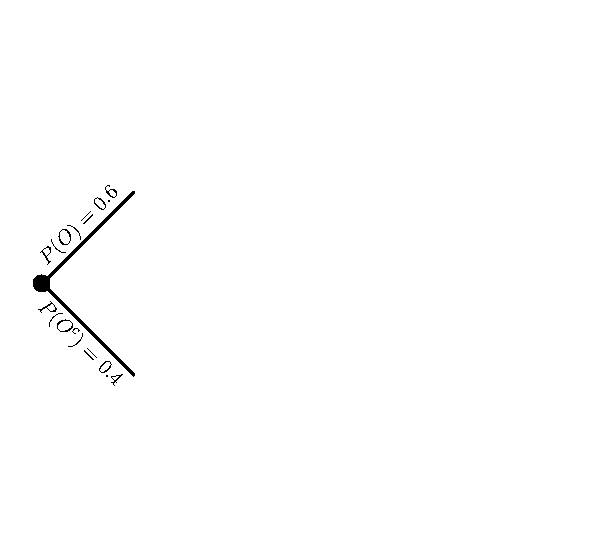
\includegraphics{chapters/chapter1/tree_diagram__branch1.pdf}}
    \caption{ }
\end{figure}

We pick the next event, say $D$, and create two branches from $O$ and two branches from $O^{c}$ for a total of four branches. 
Conditional on  $O$, two branches represent the occurrence of $D$ and occurrence of $D^{c}$.
Conditional on $O^{c}$, two branches represent the occurrence of $D$ and occurrence of $D^{c}$. 

\begin{figure}[ht!]
    \centering
    \fbox{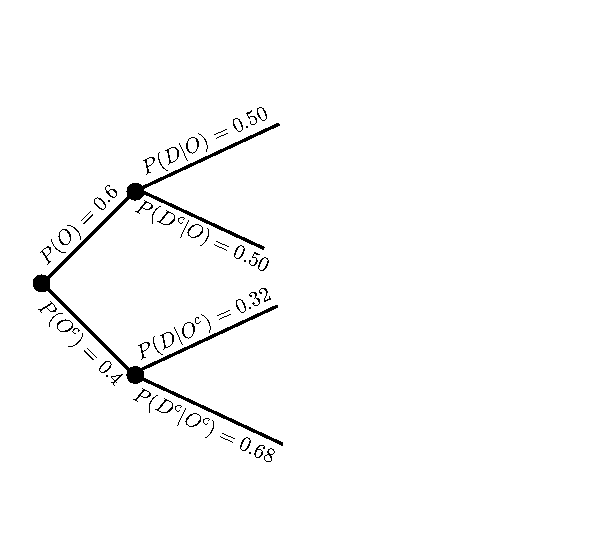
\includegraphics{chapters/chapter1/tree_diagram__branch2.pdf}}
    \caption{ }
\end{figure}

We can, in this example, do the same procedure for $S$ that we did for $D$, but this time we need to look at the occurrence of $S$ and $S^{c}$ for the four newest branches we created. 

\begin{figure}[ht!]
    \centering
    \fbox{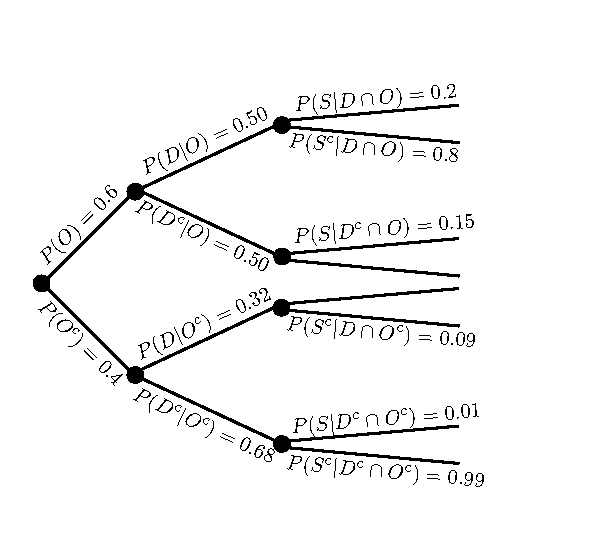
\includegraphics{chapters/chapter1/tree_diagram__branch3.pdf}}
    \caption{ }
\end{figure}


\clearpage
\subsubsection{Partitions and the law of total probability}

The multiplication rule is one way to use conditional probabilities to make computing probabilities of the intersection of many events more manageable.
We can also use conditional probabilities to simplify computing single events easier.

A \textbf{partition} of the event $A$ is a collection of sets $\mathcal{P} = \{B_{1}, B_{2}, \cdots, B_{n}\}$ such that $A = \left(A \cap B_{1}\right) \cup  \left(A \cap B_{2}\right)  \cup  \left(A \cap B_{3}\right) \cdots  \cup  \left(A \cap B_{n}\right)$ and for each $i,k$ pair of sets $B_{i} \cap B_{k} = \emptyset$.

\begin{figure}[ht!]
    \centering
    \fbox{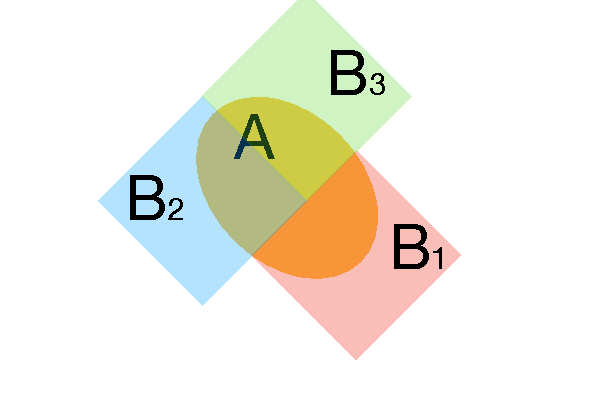
\includegraphics{chapters/chapter1/partition.pdf}}
    \caption{A partition $\mathcal{P} = \{B_{1},B_{2},B_{2}\}$ of the set $A$\label{fig.partition}}
\end{figure}


Because $B_{i}$ and $B_{k}$ are disjoint for any choice of $i$ and $k$, then $A \cap B_{i}$ and $A \cap B_{k}$ are also disjoint sets.
We can use the disjoint property of our partition to break down the probability of $A$ into the sum of probabilities of $A$ intersect $B_{k}$ for $k$ from $1$ to $n$.
\begin{align}
    P(A) &= P(\left(A \cap B_{1}\right) \cup  \left(A \cap B_{2}\right)  \cup  \left(A \cap B_{3}\right) \cdots  \cup  \left(A \cap B_{n}\right) \\
    &= P\left(A \cap B_{1}\right) +  P\left(A \cap B_{2}\right) +     + \cdots  +  P\left(A \cap B_{n}\right)  & \text{(Disjoint)}
\end{align}

We can further manipulate the above using the multiplication rule to find
\begin{align}
    P(A) &= P\left(A \cap B_{1}\right) +  P\left(A \cap B_{2}\right) +     + \cdots  +  P\left(A \cap B_{n}\right)  \\ 
         &= P(B_{1}) P(A|B_{1}) + P(B_{2}) P(A|B_{2}) + \cdots + P(B_{n}) P(A|B_{n}) 
\end{align}
This is called \textbf{the law of total probability}.
Intuitively the law of total probability says that the probability of an event $A$ can be computed by first considering the probabilities of a collection of related events, and then considering the probability that $A$ occurs given each related event. 

\ex Let $\mathcal{G} = \{(a,1), (a,2), (a,3), (b,4)\}$ and further suppose we assign the following probabilities to each outcome. 
\begin{table}[ht!]
    \centering
    \begin{tabular}{ll}
        Outcome & Probability \\
        \hline
        $(a,1)$ & 0.10\\
        $(a,2)$ & 0.25\\
        $(a,3)$ & 0.14\\
        $(b,4)$ & 0.51
    \end{tabular}
\end{table}

Define the events $A = \{ (a,1), (b,4), (a,2) \}$. The finest (as opposed to course) partition is a a collection of sets where each outcome in $A$ is in one, and only one, of the sets $B_{1},B_{2},...$. For example a partition of $A$ could be $\mathcal{P} = \{ B_{1}, B_{2}, B_{3} \}$ where $B_{1} = \{(a,1)\}$, $B_{2} = \{(b,4)\}$, and $B_{3} = \{(a,2)\}$. 
A courser partition is $\mathcal{P} = \{ B_{1}, B_{2} \}$ where $B_{1} = \{(a,1)\}$ and $B_{2} = \{(a,2),(b,4)\}$.



\subsubsection{Baye's Theorem}

We have investigated how the conditional probability is related to simultaneous events, gives us a natural definition of Independence, and can allow us to compute the probability of an event if we have a partition of that event. 

The final relationship we will explore is between two conditional probabilities. 

\textbf{Baye's Theorem} relates two conditional probabilities to one another 
\begin{align}
    P(A | B) =  \frac{P(B | A) P(A)}{P(B)}
\end{align}

We can show that Baye's theorem is true from the definition of conditional probability. 

\begin{align}
    &P(A | B) = \frac{P(A \cap B)}{P(B)}  & \text{definition} \\ 
    &P(A | B) = \frac{P(B |A) P(A)}{P(B)} & \text{multiplication rule} 
\end{align}



\subsubsection{Repeated experiments}
Many natural experiments involve repeated observations. 
It may be of interest to observe the whether and assign a probability to "sunny" or "cloudy" weather conditions. 
However, many vacationers, who plan to spend 2, 3, or more days at a remote destination may want to know the probability that the next $X$ days are sunny. 

The Cartesian product gives us a natural way to express repeated experiments.
If we chose to repeat an experiment $N$ times where each experiment produced an outcome in $\mathcal{G}$, we could imagine the set of outcomes as tuples of length $N$ where each entry in the tuple is from our sample space.
In other words, a single outcome in this repeated experiment would be $(o_{1},o_{2},o_{3},\cdots,o_{N})$ and this outcome is a member of the set $\mathcal{G} \times \mathcal{G} \times \mathcal{G} \times \cdots \times \mathcal{G}$.

Back to our vacation example. 
If a vacationer wanted to understand the chances they had of enjoying $5$ sunny days in a row, then we know that we could defined a sample space $\mathcal{G} = \{\text{"sunny"},\text{"not sunny"}\}$ and we also know that the vacationer is interested in outcomes in the sample space 
\begin{equation}
    (d_{1},d_{2},d_{3},d_{4},d_{5}) \in \mathcal{G} \times \mathcal{G}\times \mathcal{G}\times \mathcal{G}\times \mathcal{G} 
\end{equation}
where $d_{i}$ is the outcome on day $i$.
We can frame the problem, and clearly layout the potential outcomes, for example on outcome is ("sunny", "sunny", "not sunny", "sunny", "not sunny").

\subsection{The datapoint, dataset, and dataframe}

The sample space, event, and outcome are all potential results from an experiment. 
When we conduct an experiment we will generate an outcome from our sample space and call this realized outcome a \textbf{data point}. 

\ex Consider the experiment of flipping a coin and recording whether the coin lands heads or tails side up.
We can define a sample space $\samplespace = \{H,T\}$ where $H$ is an outcome that represents the coin landing heads up and $T$ represents tails up. Up until this point we have structured our experiment, but we have generated no data. We flip the coin and the coin lands tails side up. Now we have performed an experiment and generated the data point $T$.

Now suppose that we conduct an experiment with the same sample space~$(\samplespace)$ a number $N$ times and with each experiment we record a data point. A tuple of data points~$d$ is called a \textbf{data set}~$\mathcal{D} = (d_{1}, d_{2}, d_{3}, \cdots, d_{N})$ where $d_{i}$ is the data point generated from the $i^\text{th}$ experiment.
We say that we have \underline{drawn} or that we have \underline{sampled} a data set $\mathcal{D}$. Further, data points~$(d)$ are often called \underline{realized} outcomes because they are no longer in a set of potential possibilities but are now determined items. 

A data set~$\mathcal{D}$ can be unwieldy depending on the number of data points, the complexity of the sample space, or both.
A \textbf{data frame} is one way to organize a data set.
A data frame~$\mathcal{F}$ is a table where each data point~$d$ in a dataset~$\mathcal{D}$ is represented as a row in the table and if the data point is a tuple then a separate column is created for each position in the tuple.

\ex Suppose we design an experiment to collect from humans predictions, two weeks ahead from the time of our experiment, of the number of incident cases and incident deaths at the US national level of COVID-19~(\url{https://www.ncbi.nlm.nih.gov/pmc/articles/PMC7523166/}). We decide to collect from each human whether they are an expert in the modeling of infectious disease,  a prediction of incident cases, and a prediction of incident deaths. We draw a data set $\mathcal{D}$ of 50 human judgement predictions. We can organize this data set into a data frame 
\begin{table}[ht!]
    \centering
    \begin{tabular}{c|c|c}
    Expert & Prediction of cases & Prediction of deaths\\
    \hline
    Yes     & 145    & 52 \\ 
    No      & 215    & 34 \\
    Yes     & 524    & 48 \\
    Yes     & 265    & 95 \\
    No      & 354    & 35 \\
    \end{tabular}
    \caption{Example data frame $\mathcal{F}$ built from a data set~$\mathcal{D}$ that contains 5 data points where each data point is a tuple of length three.}
\end{table}

Above, the first data point is $(Yes,145,52)$, the second data point is $(No, 215, 34)$, and so on until the last data point $(No, 354, 35)$. A data frame can also include informative information for others such as labels for each column.


\section{Exercises}

\begin{enumerate}
    \item \begin{align*}
              A &= \{1,2,3,4,5,6\};
              \;\;B = \{1,3,6\} \\
              C &= \{7\}  
              \;\;D = \emptyset
           \end{align*}
    \begin{enumerate}
        \item Please compute $A \cap B$
        \item Please compute $A \cup C$
        \item Please compute $A \cup D$
        \item Please compute $A \cap D$
        \item Please compute $(A \cap B) \cup (C \cup D)$
    \end{enumerate}
    \item Let the sample space $\mathcal{G} = \{ 1,2,3,4,5,6,7 \}$
    \begin{enumerate}
       \item Please compute $A^{c}$
       \item Please compute $B^{c}$
       \item Please compute $D^{c}$
       \item Please compute $\mathcal{G} \cap A$
       \item Is $A \subset \mathcal{G}$?
       \item Is $\emptyset \subset \mathcal{G}$?
    \end{enumerate}
    
    \item Let the sample space $\samplespace = \{0,1,2,a,b,c\}$ and let $A=\{0,1\}$, $B=\{x | x\text{ is a letter of the English alphabet}\}$
    \begin{enumerate}
        \item Please compute $A \cap B$
        \item Please compute $A \cup B$
        \item Please compute $A^{c}$
        \item Is $A \cup B = \samplespace$?
        \item If we assigned probabilities to all outcomes, could $P(A \cup B) = 1$? why or why not?
    \end{enumerate}
    
    \item Let $A = {0,1,2}$ for some sample space $\mathcal{G} = \{0,1,2,3,4,5,6\}$. Further assume $P(A) = 0.2$. 
    \begin{enumerate}
        \item Are the sets $A$ and $A^{c}$ disjoint? Why or why not.
        \item Simplify $P(A \cup A^{c})$ into an expression that involves $P(A)$ and $P(A^{c})$.
        \item Use Kolmogorov's axioms to show that $P(A) = 1 - P(A^{c})$ 
    \end{enumerate}
    
    \item Let $\samplespace = \{x | x\text{ is a positive integer}\}$
    \begin{enumerate}
        \item Are the sets $\emptyset$ and $\samplespace$ disjoint?
        \item Simplify $P(\samplespace \cup \emptyset)$ into an expression that involves $P(\samplespace)$ and $P(\emptyset)$
        \item Use Kolmogorov's axioms to show that $P(\emptyset) = 0$
    \end{enumerate}
    
    \item If $A=\{1,2,3\}$ and $B = \{2,3,4\}$ and $C = \{1,3\}$
    \begin{enumerate}
        \item Can $P(A) < P(B)$? Why or why not
        \item Can $P(A) < P(C)$? Why or why not
    \end{enumerate}
    \item Use what you know about the intersection, about subsets, and about probability to show that $P(A \cap B) \leq P(A)$. Hint: How are $A \cap B$ and $A$ related?
    \item Suppose we wish to study the reemergence of cancer among patients in remition. We collect data on 1,000 patients who are in cancer remition and follow them for 5 years. At five years we are interested in the probability of a second cancer. 
    \begin{enumerate}
        \item Define a sample space $\mathcal{G}$ we can use to assign probabilities to a second cancer and no second cancer. 
        \item After five years of followup we find that 238 patients experienced a second cancer. Use the frequentist approach to assign probabilities to a second cancer \underline{and} no second cancer.
        \item If you collected data on 2,000 patients do you expect the probability of a second cancer to change? How do you expect the probability to be different for 2,000 patients than with 1,000 patients? 
    \end{enumerate}
    
   \item A study (link = \href{here}{https://www.science.org/doi/10.1126/science.abj8222} found that young adults were 32 times more at risk to develop multiple sclerosis (MS) after infection with the Epstein-Barr virus compared to young adults who were not infected by the virus. The experiment enrolled 10 million young adults and observed them for a period of 20 years.
   \begin{enumerate}
       \item Design a sample space if we wish to study outcomes that describe the number of young adults who develop MS. 
       \item Build the event $(E_{1})$ "less than 10\% of young adults develop MS" using set notation.
       \item Build the event $(E_{2})$ "less than 5\% of young adults develop MS" using set notation.
       \item Are $E_{1}$ and $E_{2}$ disjoint? Why or why not?
       \item Can $P(E_{1}) < P(E_{2})$?
   \end{enumerate}
   
   \item Please compute the following
   \begin{enumerate}
       \item $A = \{1,2,3\}$ and $B = \{4,5,6\}$. Please compute $A \times B$ (Answer should be a set of tuples)
       \item $A = \{1,2,3\}$. Please compute $A \times A$ (Answer should be a set of tuples)
       \item How many elements are in $A \times A$ (looking for a number)
       \item How many elements are in  $A \times A \times A$? (looking for a number)
       \item How many elements are in  $A \times A \times A \times \cdots \times A$ where we take the Cartesian product $N$ times? (looking for a number)
   \end{enumerate}
   \item Define a sample space $\samplespace = \{ a,b,c,d,1,2,3,4,5 \}$ and let $E_{1} = \{1,3,5\}$, $E_{2} = \{a,b,c\}$, $E_{3} = \{ a,d,5 \}$. We further assign the following probabilities 
   \begin{table}[ht!]
       \centering
       \begin{tabular}{ c c}
       Outcome &  $P(\{\text{Outcome}\})$\\
       \hline
            a & 0.10  \\
            b & 0.05 \\
            c & 0.15 \\
            d & 0.02 \\
            1 & 0.14 \\
            2 & 0.25 \\
            3 & 0.08 \\
            4 & 0.04 \\
            5 & 0.17
       \end{tabular}
   \end{table}
   \begin{enumerate}
       \item Compute $P(E_{1})$ (looking for a number)
       \item Compute $P(E_{2})$ (looking for a number)
       \item Compute $P(E_{3})$ (looking for a number)
       \item Compute $P(E_{1} \cap E_{2})$ (looking for a number)
       \item Compute $P(E_{1} \cap E_{3})$ (looking for a number)
       \item Compute $P(E_{2} \cap E_{3})$ (looking for a number)
       \item Compute $P(E_{1} | E_{2})$ (looking for a number)
       \item Compute $P(E_{1} | E_{3})$ (looking for a number)
       \item Compute $P(E_{2} | E_{3})$ (looking for a number)
       \item Compute $P(E_{3} | E_{2})$ (looking for a number)
   \end{enumerate}
   \item Define a sample space $\samplespace = \{ (a,1),(b,1),(c,1),(a,2),(b,2),(c,2) \}$ and let $E_{1} = \{(a,1),(a,2),(c,2)\}$, $E_{2} = \{(c,2),(a,1) \}$, $E_{3} = \{(b,2) \}$. We further assign the following probabilities 
   \begin{table}[ht!]
       \centering
       \begin{tabular}{ c c}
       Outcome &  $P(\{\text{Outcome}\})$\\
       \hline
            (a,1) & 0.05  \\
            (b,1) & 0.22 \\
            (c,1) & 0.15 \\
            (a,2) & 0.02 \\
            (b,2) & 0.13 \\
            (c,2) & 0.43 \\
       \end{tabular}
   \end{table}
   \begin{enumerate}
       \item Compute $P(E_{1})$ (looking for a number)
       \item Compute $P(E_{2})$ (looking for a number)
       \item Compute $P(E_{3})$ (looking for a number)
       \item Compute $P(E_{1} \cap E_{2})$ (looking for a number)
       \item Compute $P(E_{1} \cap E_{3})$ (looking for a number)
       \item Compute $P(E_{2} \cap E_{3})$ (looking for a number)
       \item Compute $P(E_{1} | E_{2})$ (looking for a number)
       \item Compute $P(E_{1} | E_{3})$ (looking for a number)
       \item Compute $P(E_{2} | E_{3})$ (looking for a number)
       \item Compute $P(E_{3} | E_{2})$ (looking for a number)
   \end{enumerate}
   
   \item Given two events $A$ and $B$, show that $P(A|B) \geq P(A \cap B)$ (looking for a short explanation and mathematical argument)
   
   \item Suppose we wish to study adverse outcomes among patients who have unprotected left main disease~(\url{https://www.nejm.org/doi/full/10.1056/nejmoa1909406}). In this experiment~(called a clinical trial) we randomize patients to receive percutaneous intervention~(PCI) or a coronary artery bypass graft~(CABG). We wish to study the number of patients who received a PCI \underline{and} experienced a myocardial infarction~(MI) between the time they had their procedure and 5 years, however we only know three pieces of information: (i) the probability a patient was randomized to PCI was 0.5, (ii) the probability a patient was randomized to CABG was 0.5, and (iii) we know that the probability of a MI was 0.2 among patients who received a PCI.
   \begin{enumerate}
       \item Define a sample space that will allow us to compute the probability a patient was randomized to PCI and experienced an MI (looking for a description of the sample space and a set)
       \item Please compute the probability a patient experiences an MI and was randomized to PCI. (looking for a number)
       \item Please compute the probability a patient does not experience an MI and was randomized to PCI. (looking for a number)
   \end{enumerate}
   
   \item If two events $A$ and $B$ are disjoint, are they also independent? (looking for a description and mathematical argument to backup your description.)
   
   \item Researchers studied epidemiological characteristics of a variant of SARS-CoV-2 called B.1.526~(\url{https://www.science.org/doi/10.1126/sciadv.abm0300}). Suppose we too wanted to study the impact of B.1.526 on a population of patients who have been admitted to the hospital for COVID-19 by collecting each patient's age, whether they have were vaccinated against COVID-19, and whether their infection was due to the B.1.526 variant.
   
   \begin{enumerate}
       \item If we define our experiment as generating the above three pieces of information from a single patient, define a sample space~($\samplespace$) for these potential outcomes. (looking for a short description and the sample space)
       \item Define a sample space if we repeated our above experiment 2 times. In other words, what would be our sample space if we collected information from 2 patients? 
   \end{enumerate}
    
   \item Can a data set ever have more elements than a sample space? Explain. (looking for a paragraph with some examples)
   
   \item Suppose we collect the following data about the co-occurence of patients admitted to the hospital for influenza-like illness~(ILI) and whether the patient does or does not work in a clinical setting. 
   After data collection we estimate the following probabilities: The probability that a patient works in a clinical setting is 0.12. The probability that a patient who works in a clinical setting is admitted to the hospital for ILI is 0.2, and the probability a patient who does not work in a clinical setting was admitted to the hospital for ILI is 0.3. 
   \begin{enumerate}
       \item Define a sample space to study outcomes related to the co-occurance of ILI/No ILI and patients who do/do not work in a clinical setting. (Looking for a set and a very brief description of an outcome or two.) 
       \item Compute the probability a patient is admitted to the hospitals for ILI and they work in a clinical setting. (Looking for an equation and number)
       \item Compute the probability a patient is not admitted to the hospital for ILI and they work in a clinical setting. (Looking for an equation and number)
       \item Compute the probability a patient is admitted to the hospital for ILI and they do not work in a clinical setting. (Looking for an equation and number)
       \item Compute the probability a patient is not admitted to the hospital for ILI and they do not work in a clinical setting. (Looking for an equation and number)
   \end{enumerate}
   
   \item Show that for two events $A$ and $B$ the $P(A|B)P(B)  \leq P(B)$. Why is this the case intuitively? (Looking for two brief descriptions)
   \clearpage
   \item \begin{figure}[ht!]
       \centering
       \fbox{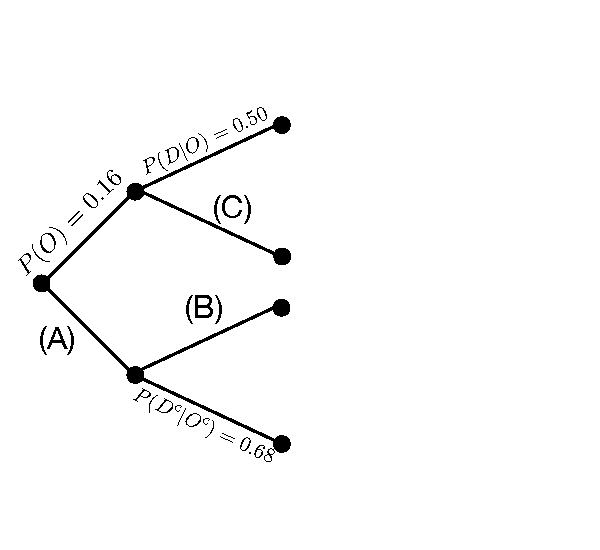
\includegraphics{chapters/chapter1/tree_diagram__HW.pdf}}
   \end{figure} Please use the above tree diagram to answer the following questions. 
   \begin{enumerate}
       \item Fill in the $P(O^{c})$ which corresponds to (A) in the figure
       \item Fill in the $P(D | O^{c})$ which corresponds to (B) in the figure
       \item Fill in the $P(D^{c} | O)$ which corresponds to (C) in the figure
       \item Please compute $P(D)$
       \item Please compute $P(D^{c})$
   \end{enumerate}
   
   \item Influenza is a contagious virus that enters the respiratory system from a human's nose, throat, or lungs. Common symptoms are cough, chills, and a fever.
   Suppose we collect data from a local hospital about those who were infected and not infected by the influenza virus and the above three symptoms. Let $\samplespace = \{ (x,y)  | x \text{ is } \text{"Flu"} \text{ or } \text{"not Flu"} \text{ and } y \in \{ \text{cough },\text{chills },\text{ fever} \}   \}$. 
   Suppose further that we define events $F$ = \{ (x,y)  | x \text{ is } \text{"Flu"} \}, $C$ = \{ (x,y)  | y \text{ is } \text{"Cough"} \}, $H$ = \{ (x,y)  | y \text{ is } \text{"Chills"} \} , $E$ = \{ (x,y)  | y \text{ is } \text{"Fever"} \}, and that $P( C|F ) = 0.5$ and $P( C|F^{c} ) = 0.15$, $P( H|F ) = 0.25$ and $P( H|F^{c} ) = 0.01$, $P( E|F ) = 0.98$ and $P( E|F^{c} ) = 0.35$, $P(F) = 0.02$  
    \begin{enumerate}
       \item A patient presents with the chills. What is the probability they have influenza? 
       \item What symptom from the above, if present, would indicate with a high probability a patient has influenza?
    \end{enumerate}
    
\end{enumerate}

\section{Student contributions}


\textit{Jessica Berman - Class of 2025-Advice:} When I see a problem pertaining to conditional probability it helps me to talk the question out and actually say to myself “what is the probability of A given B has already occured” because P(A|B) is not clear to me without saying it aloud.

\textit{Jessica Berman - Class of 2025-Example:} A fun fact about conditional probability is that it is used in politics. For example, if there are 4 candidates running in a presidential election, the chances of winning for each of them is 25%. However, given that one candidate drops out of the race two weeks later, the candidates' probability of winning changes to 33.33% each (P(Win | One candidate drops out)).



\section{Glossary}
\begin{Glossary}
\item[Set]
\item[Subset]
\item[Set equality]
\item[Set intersection]
\item[Set union]
\item[Universal set]
\item[Empty set]
\item[Sample space]
\item[Experiment]
\item[Outcome]
\item[Event]
\item[Probability]
\item[Kolmorogov's Axioms]
\item[Principle of Equally Likely Outcomes]
\item[Product Set]
\item[Compound event]
\item[Conditional probability]
\item[Multiplication Rule]
\item[Independence]
\end{Glossary}







\chapterauthor{thomas mcandrew}{Lehigh University}
%\chapterauthor{Second Author}{Second Author Affiliation}
\chapter{Random variables}
\hspace{1mm}

\section{Introduction}\label{intro}

The foundations of probability are built on sets,
yet data is more naturally stored and more easily computed on if it is represented numerically.  

Random variables match each outcome in our sample space to a value on the number line. 

In addition to computational advantages, random variables help us extract from our data the most important characteristics, and they serve as building blocks which we can use to create powerful models.
Random variables are also a language we can use to communicate our modeling efforts to other mathematicians, statisticians, and data scientists.  

Suppose we hypothesize that the frequency of social media posts on some popular outlet are related to influenza-like illness~(ILI)---a syndromic diagnosis suggesting a patient may have influenza. A patient is diagnosed with ILI if their temperature is measured to be at or above 38C and symptoms resembling the flu.
Because influenza is most active in winter and spring, we collect a random sample, each day, of social media posts from September to May and in addition we collect the proportion of patients who are admitted to the hospital and are diagnosed with influenza-like illness at the US national level. 

The above hypothesis, data collection, and future inference has numerous details. 
However, we will see shortly that we can simplify our hypothesis by using random variables. 

\section{Maps from the sample space to the number line}\label{maps}

Given a sample space $\mathcal{G}$, a \textbf{random variable}, (e.g. $X$), is a function from each element in $\mathcal{G}$---from each outcome---to a value on the real number line.
The real number line contains all numbers: integer and decimal, from negative to positive infinity.

\textbf{Example:} Suppose our sample space contains two elements $\mathcal{G} = \{ a,b \}$. We may decide to define a random variable $X$ that maps the outcome $a$ to the value $-1$ and the outcome $b$ to the value $1$. In otherwords, $X(a)=-1$ and $X(b)=1$. We could as well define a random variable $Y$ on the same sample space such that $Y(a)=0$ and $Y(b)=1$.

\textbf{Example:} Suppose our sample space contains all integers from 0 to 1000 $\mathcal{G} = \{0,1,2,3\cdots,1000 \}$. We may be most interested in when an integer is even or odd, and so we can define a random variable $Y(y)=0$ when $y$, our outcome, is an odd integer and $Y(y)=1$ when $y$ is even. This is an example of how a random variable can distill down a sample space with many outcomes into a random variable with two.

\textbf{Example:} Suppose we decide to study the relationship between the cumulative total number of cigarettes smoked by a person form the date that they started smoking and the presence of lung cancer.
We define our sample space to be $\mathcal{G} = \{ (x,y) | x \in \mathbb{Z}, y \in \{0,1\} \}$. We define two random variables, a random variable $X$ that maps the outcome $(x,y)$ to the value in the first position $x$, and a random variable $Y$ that maps the $outcome (x,y)$ to the value in the second position $y$. Though our outcomes are linked, we can use random variables to think about two separate outcomes---cigarettes smoked and lung cancer---and how they interact.

\section{A new sample space}\label{intro}

When we build a random variable $(X)$ that maps outcomes to values on the number line we create a new sample space which we will call the support of $X$ or $supp(X)$. 
Define a sample space $\mathcal{G}$ without outcomes $o_{i}$.
Then the \textbf{support of X} is
\begin{align}
    supp(X) = \{x | X(o) = x \text{ for some outcome } o \text{ in } \mathcal{G} \}
\end{align}
Our new sample space is the set of all the potential values that our random variable $X$ can produce.
This is a sample space linked to $\mathcal{G}$, but in practice after we develop a random variable we often no longer reference $\mathcal{G}$.

\ex In our above example where $\mathcal{G} = \{a,b\}$, the random variable $X$ has support $supp(X) = \{-1,1\}$ and $supp(Y)=\{0,1\}$.
Lets look at another example, when above $\mathcal{G}$ is  the set of all integers from 0 to 1000. 
Even though the sample space is quite large, the random variable that maps the integers to 0 when they are odd and 1 when even has a small support $(supp(Y) = \{0,1\})$.   

\section{How to assign probabilities to a random variable}

Random variable themselves do not require that we include the probability of each of their values. Random variables are a function from outcomes to the real numbers---nothing more. 
That said, in practice we build random variables expecting that the probabilities we assign to outcomes in our sample space will correspond to probabilities assigned to values of our random variable.

We assign a probability to the value $x$, which belongs in the support of random variable $X$, the sum of the probabilities of all the outcomes that $X$ maps to $x$.
\begin{equation}
    P(X=x) = P(o_{1}) + P(o_{2}) + \cdots + P(o_{n})    
\end{equation}
where each outcome $o_{1},o_{2},\cdots,o_{n}$ is mapped by $X$ to the value $x$. In other words, $X(o)=x$ for each of $o_{1},o_{2},\cdots,o_{n}$.

\ex Define a $\samplespace = \{a,b,c,d,e\}$ and a random variable $X$ that maps the outcomes to the following values
\begin{table}[ht!]
    \centering
    \begin{tabular}{ccc}
        Outcome & P(outcome) & X(outcome)  \\
        \hline
        a & 0.1  & 0\\
        b & 0.25 & 1\\
        c & 0.15 & 1\\
        d & 0.3  & 2\\
        e & 0.2  & 0\\
    \end{tabular}
\end{table}

We assign the probability that $X=0$ as the sum of the probabilities assigned to outcome $a$ and outcome $e$, or
\begin{align}
    P(X=0) &= P(\{a\}) + P(\{e\})\\
           &= 0.1+0.2 = 0.3
\end{align}
We can run the same procedure for all the elements in the support of $X$, 
\begin{align}
    P(X=1) &= P(\{b\}) + P(\{c\})\\
           &= 0.25+0.15 = 0.40\\
    P(X=2) &= P(\{d\}) = 0.3 = 0.30,
\end{align}
and organize our work in a table
\begin{table}[ht!]
    \centering
    \begin{tabular}{c|c}
        X & P(X=x) \\
        \hline
        0 & 0.30\\
        1 & 0.40\\
        2 & 0.30
    \end{tabular}
\end{table}

A \textbf{probability distribution} for a random variable $X$ is a set of tuples where the first position in each tuple is a value in the support of $X$ and the second position in the tuple is the corresponding probability assigned to that value. 

\ex A probability distribution for the random variable $X$ above is $\{(0,0.30),(1,0.40),(2,0.30)\}$.

\ex Imagine we run an experiment that collects data on marathon runners. We decide to collect the number of elapsed minutes until they finish the race. Our sample space is defined as all positive integers $\samplespace = \{1,2,3,\cdots,\}$. We may decide to build a random variable $X$ that maps outcomes less than 60 to the value 1, outcomes from 61 to 120 to the value 2, and outcomes greater than 120 to the value 3. One potential probability distribution for $X$ is $\{(1,0.10),(2,0.50),(3,0.40)\}$. For this probability distribution, $P(X=1) = 0.10$, $P(X=2) = 0.50$, and $P(X=3) = 0.40$.

\begin{figure}[ht!]
    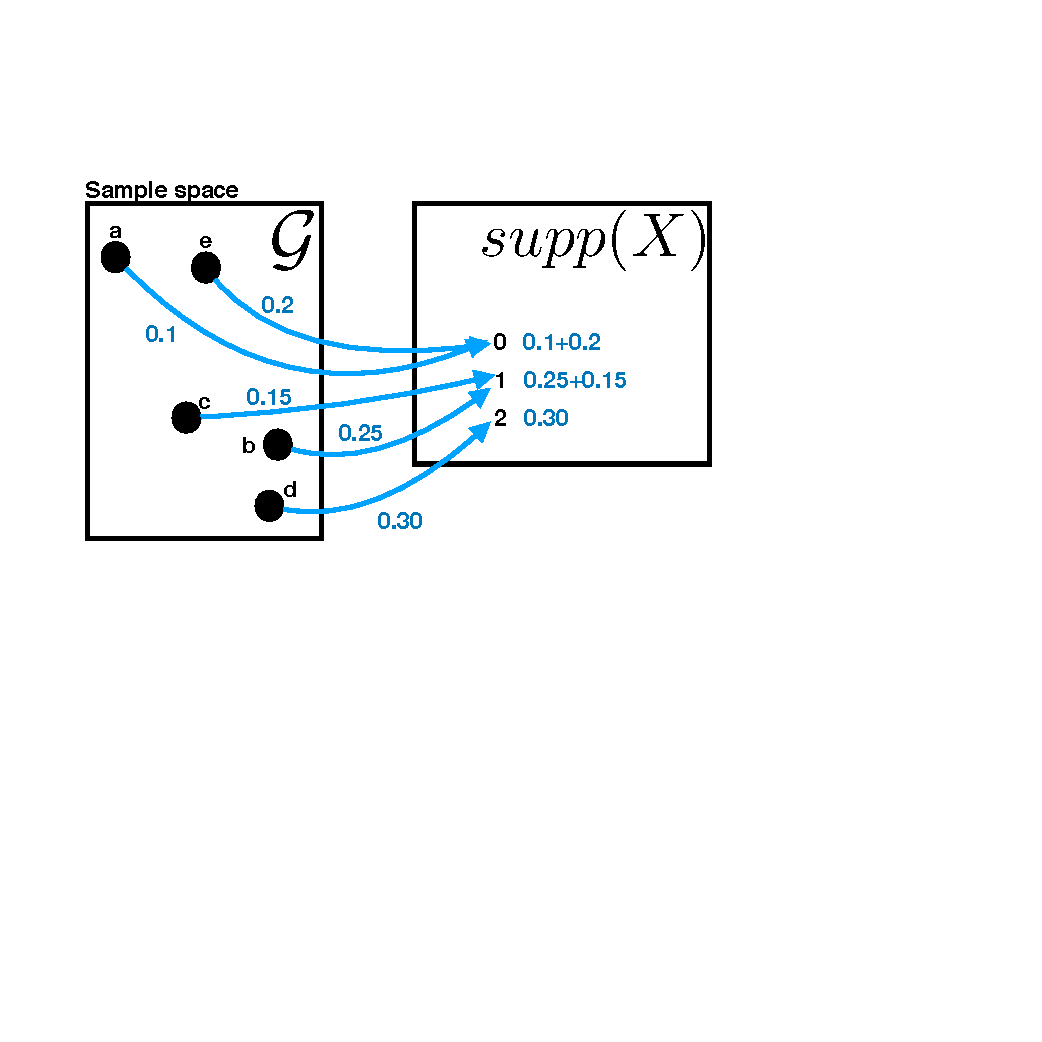
\includegraphics{chapters/chapter2/rvsLink.pdf}
    \caption[List]{A sample space $\samplespace$ with elements $\{a,b,c,d,e\}$ and a random variable $X$ that maps each element in $\samplespace$ to one the values: 0, 1, or 2. Probabilities corresponding to outcomes in the sample space and how they map to probabilities for each value of $X$ are shown in blue.}
\end{figure}

\section{Probability mass function}

There are several supportive tools that we can use to help us better understand random variable we create.
The first is the probability mass function, or p.m.f.
The \textbf{probability mass function} is a \underline{function} that maps values in the support of a random variable $X$ to their corresponding probabilities.
Inputs are values of $X$, outputs are probabilities.

The probability mass function is a convenient way to organize a probability distribution and it allows us to transfer all the information we know about functions to random variables.

\ex Define a random variable $Y$ with support $\{-1,0,1\}$, probability distribution \{(-1,0.2),(0,0.5),(1,0.3)\}, and probability mass function 
\begin{equation}
    f(y) = \begin{cases}
            0.2 & \text{ when } y=-1\\
            0.5 & \text{ when } y = 0\\
            0.3 & \text{ when } y=1
            \end{cases}
\end{equation}
The function---our probability mass function---is a type of function called a \textbf{piecewise} function.

We can ask our pm.f. to return the probability for a given value
\begin{equation}
    f(1) = 0.3
\end{equation}
and we can visualize our probability mass function using, for example, a barplot.
\begin{figure}[ht!]
    \centering
    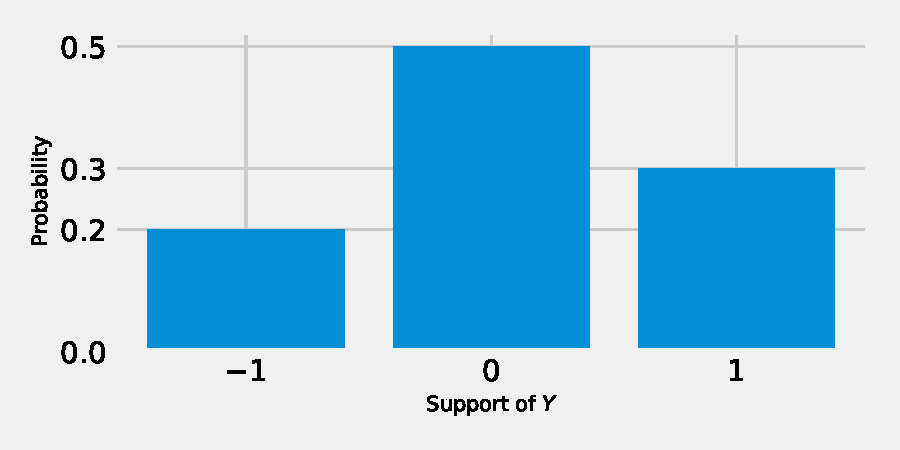
\includegraphics{chapters/chapter2/pmfviz.pdf}
    \caption{A barplot for visualizing the probability mass function of our random variable $Y$. The support of $Y$ is plotted on the horizontal axis and height of each bar corresponds to the probability assigned to that value in the support.\label{fig.pmfviz}}
\end{figure}

\textbf{Distributed as $f$:} Because we can use the probability mass function to describe the probability distribution of a random variable, we will often write 
\begin{equation}
    Y \sim f
\end{equation}
The above formula is read "the random variable $Y$ is distributed as $f$", and what we mean when a random variable is distributed as $f$ is that the support of $Y$ is the same as the domain of the function $f$ and that the probability of a value $y$ is equal to $f(y)$, or 
\begin{align}
    supp(Y) &= dom(f)\\
    P(Y = y) &= f(y)
\end{align}

The probability mass function is a convenient method for assigning probabilities to random variables and visualizing the distribution of a random variable.

\section{Cumulative mass function}

The \textbf{cumulative mass function} is a \underline{function} that maps values in the support of a random variable $X$ to the probability that the random variable is less than or equal to this value, or $P(X \leq x)$.

We use a capital $F$ to denote a cumulative mass function (c.m.f).
The c.m.f. corresponding to random variable $X$ has a domain equal to the support of $X$ and produces values between 0 and 1 (the values a function can produce is called the function's \textbf{image}). 

\begin{align}
    supp(X) &= dom(F)\\
    image(F) &= [0,1]\\
    P(X \leq x) &= F(x)
\end{align}

The c.m.f. too can be visualized and we could also use the c.m.f. to describe the probability distribution of a random variable. 
This is because we can use the c.m.f. to derive the p.m.f.

\begin{figure}[ht!]
    \centering
    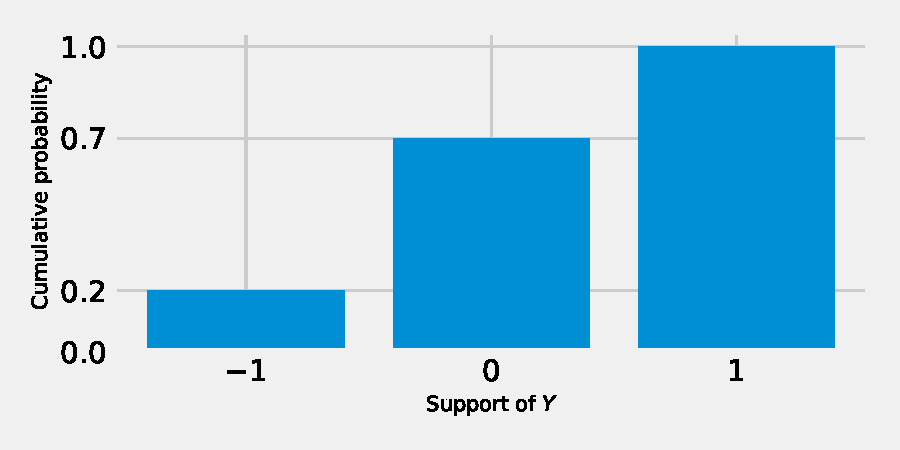
\includegraphics{chapters/chapter2/cmfviz.pdf}
    \caption{A barplot for visualizing the cumulative mass function of our random variable $Y$. The support of $Y$ is plotted on the horizontal axis and height of each bar corresponds to the probability assigned to values $(v)$ less than or equal to $v$ in the support.\label{fig.pmfviz}}
\end{figure}


\ex For a random variable 
\begin{align}
    X &\sim f\\
    supp(X) &= \{0,1,2,3\}\\
    f(x) &= \begin{cases}
     0 & 0.1\\
     1 & 0.3\\
     2 & 0.2\\
     3 & 0.4\\
    \end{cases}
\end{align}
The c.m.f is then 
\begin{align}
    F(x) =  
    \begin{cases}
     0 & 0.1\\
     1 & 0.3 + 0.1 = 0.4\\
     2 & 0.2+0.3+0.1 = 0.6\\
     3 & 0.4+0.2+0.3+0.1 = 1\\
     \end{cases}
\end{align}

We can use the c.m.f $(F(x))$ to compute any p.m.f ($f(x)$) too by noticing that for a support $\{x_{0},x_{1},x_{2},x_{3}, \cdots,x_{n-1}\cdots,x_{n}\}$ where the values in this set are ordered form smallest to largest 
\begin{align}
    f(x_{i}) &= \left[f(x_{i}) + f(x_{i-1}) + \cdots f(x_{0}) \right] - \left[f(x_{i-1}) + \cdots f(x_{0})\right] \\ 
    &=F(x_{i}) - F(x_{i-1}).
\end{align}
Because the p.d.f. and c.m.f equivalently describe the probability distribution of a random variable we can write $X\sim F$ or $X \sim f$.  

\section{Two or more random variables}

A single random variable is a useful way to describe a sample space and the probabilities assigned to values on the number line corresponding to outcomes.

But more complicated scientific questions often require several random variables and rules for how they interact.
We will explore how to generate multiple random variables  on the same sample space. 
Then we will develop an approach to define probabilities for combinations of random variables, a joint probability mass function and joint cumulative mass function.

Suppose we design a sample space $\samplespace$ and build two random variables on this space $X$ and $Y$.
Because $X$ and $Y$ are random variables we can think of the support of $X$ and support of $Y$ as two new sample spaces. Lets assume that the outcomes in $supp(X) = \{x_{1},x_{2},x_{3},\cdots,x_{N}\}$ and that the outcomes in $supp(Y) = \{y_{1},y_{2},\cdots,y_{M}\}$. 
Then we can define a new set of outcomes in the space $supp(X) \times supp(Y) = \{x_{i}, y_{j}\}$ for all combinations of $i$ from $1$ to $N$ and $j$ from $1$ to $M$.

This new space above maps outcomes in $\samplespace$ to a tuple $(x_{i},y_{j})$  where the outcomes were mapped by $X$ to the value $x_{i}$ and by $Y$ to the value $y_{j}$. 
If we assign the probability of $(x_{i},y_{j})$ to be the the sum of the probabilities of all outcomes in $\samplespace$ that $X$ maps to $x_{i}$ and $Y$ maps to $y_{i}$ then we call this a \textbf{joint probability distribution}. 

\ex A pharmaceutical company launches a clinical trial to study adverse events from a novel medicine. The trial enrolls patients and randomizes them to receive the novel drug or optimal medical therapy. The trial expects three potential adverse events which we call $\text{ae}_{1}$, $\text{ae}_{2}$, and $\text{ae}_{3}$.
We may choose to define a sample space $\samplespace = \{(\text{nov},\text{ae}_{1}),(\text{nov},\text{ae}_{2}),(\text{nov},\text{ae}_{3}),(\text{omt},\text{ae}_{1}),(\text{omt},\text{ae}_{2}),(\text{omt},\text{ae}_{3})\}$ and further build a random variable $X$ that maps outcomes to values 0 when an adverse event was experienced by a control patient and 1 when an adverse event was experienced by a novel drug patient, and a random variable $Y$ that maps adverse event 1 to the value 1, adverse event 2 to the value 2, and adverse event 3 to the value 3.
\begin{align*}
    \samplespace = \{(\text{nov},\text{ae}_{1}),(\text{nov},\text{ae}_{2}),(\text{nov},\text{ae}_{3}),(\text{omt},\text{ae}_{1}),(\text{omt},\text{ae}_{2}),(\text{omt},\text{ae}_{3})\}
\end{align*}

\begin{table}[ht!]
    \centering
    \begin{tabular}{c|c}
        Event & X \\
        \hline
        $(\text{nov},\text{ae}_{1})$ & 1\\
        $(\text{nov},\text{ae}_{2})$ & 1\\
        $(\text{nov},\text{ae}_{3})$ & 1\\
        $(\text{omt},\text{ae}_{1})$ & 0\\
        $(\text{omt},\text{ae}_{2})$ & 0\\
        $(\text{omt},\text{ae}_{3})$ & 0\\
    \end{tabular}
\end{table}

\begin{table}[ht!]
    \centering
    \begin{tabular}{c|c}
        Event & Y \\
        \hline
        $(\text{nov},\text{ae}_{1})$ & 1\\
        $(\text{nov},\text{ae}_{2})$ & 2\\
        $(\text{nov},\text{ae}_{3})$ & 3\\
        $(\text{omt},\text{ae}_{1})$ & 1\\
        $(\text{omt},\text{ae}_{2})$ & 2\\
        $(\text{omt},\text{ae}_{3})$ & 3\\
    \end{tabular}
\end{table}

A joint probability distribution would assign probabilities to all possible pairs of values for $X$ and $Y$. 

\begin{table}[ht!]
    \centering
    \begin{tabular}{c c | c}
        X & Y & prob \\
        \hline
        1 & 1 & 0.1\\
        1 & 2 & 0.05\\
        1 & 3 & 0.23\\
        0 & 1 & 0.05\\
        0 & 2 & 0.30\\
        0 & 3 & 0.27
    \end{tabular}
\end{table}

We write $P(X=x, Y=y)$ to denote the probability assigned to the joint probability that the random variable $X$ equals the value $x$ and the random variable $Y$ equals the value $y$. With the above example in mind, $P(X=0,Y=2) = 0.30$ and this probability could be described as the probability an OMT patient experiences adverse event 2.

Joint probability distributions are often visualized as a table with one random variable's values representing the rows and the second random variable's values representing the columns

\begin{table}[ht!]
    \centering
    \begin{tabular}{c|ccc}
             & Y = 1 & Y = 2 & Y = 3 \\
             \hline
    X=0    & 0.05  & 0.30  & 0.27  \\
    X=1    & 0.10  & 0.05  & 0.23 
    \end{tabular}
\end{table}

A joint distribution can be used to compute probabilities that the random variable $X$ equals the value $x$ for any value of $Y$---$P(X=x)$ and also the probability that the random variable $Y$ equals the value $y$ for any value of $x$---$P(Y=y)$.
These probabilities are called \textbf{marginal probabilities}.  

The marginal probabilities that $X$ equals $0$, or $P(X=0)$, is computed by summing the joint probabilities where $X=0$. We can use the same procedure to compute the marignal probability that $X=1$. 

\begin{align*}
    P(X=0) &= P(X=0,Y=1) + P(X=0,Y=2) + P(X=0,Y=3)\\
           &= 0.05+0.30+0.27 = 0.62\\
    P(X=1) &= P(X=1,Y=1) + P(X=1,Y=2) + P(X=1,Y=3) \\
           &= 0.10+0.05+0.23 = 0.38 \\
\end{align*}

The same procedure can be done for the random variable $Y$ to find marginal probabilities:

\begin{align*}
    P(Y=1) &= P(X=0,Y=1) + P(X=1,Y=1)\\
           &= 0.1+0.05 = 0.15 \\
    P(Y=2) &= P(X=0,Y=2) + P(X=1,Y=2)  \\
           &= 0.05+0.30 = 0.35 \\
    P(Y=3) &= P(X=0,Y=3) + P(X=1,Y=3)  \\
           &= 0.23+0.27 = 0.50\\
\end{align*}

Joint distributions need not be restricted to only two random variables. 
We can build joint distributions of any number of random variables and can compute marginal probabilities in the same way that we do for a joint distribution of two random variables.

The rules, laws, and theorems of probability that we learned in chapter one carry over to random variables.
This is because we can consider a new sample space of values that our random variable can take. 
Suppose we build two random variables $X$ that maps outcomes to the the values -1,0,1 and $Y$ that maps outcomes to the values 1,2,3. 
We can define a new sample space $\samplespace = \{(x,y) | x \in supp(X) \text{ and } y \in supp(Y) \}$
With our new sample space, we can now discuss statements like $P(X = x | Y = y)$. 

\ex If we continue with our pharmaceutical example, we can build a new sample space $\samplespace = \{(0,1),(0,2),(0,3),(1,1),(1,2),(1,3)\}$ and compute, for example, $P(X=1 | Y=2) = \frac{P(X=1,Y=2)}{P(Y=2)} = \frac{0.05}{0.35} = 0.14$.

We can define the conditional probability of the value of one random variable given another as 
\begin{align}
    P(A =a | B =b) = \frac{P(A=a,B=b)}{P(B=b)}
\end{align}

and so define statistical independence between two random variables, $A$ and $B$, as 
\begin{align}
    P(A = a | B=b) = P(A = a) \text{ for all } a \in supp(A),b \in supp(B)    
\end{align}

We can also translate the law of total probability from events to random variables.
For a partition $[Y=y_{1}] \cup [Y=y_{2}] \cup [Y=y_{3}] \cup \cdots \cup [Y=y_{n}]$ of the event that the random variable $X=x$,
\begin{align}
    \begin{aligned}
    P(X=x) = P(X=x|Y=y_{1})p(y_{1}) + P(X=x|Y=y_{2})p(y_{2})\\ + P(X=x|Y=y_{3})p(y_{3}) \cdots + P(X=x|Y=y_{n})p(y_{n})
    \end{aligned}
\end{align}

By thinking of the values of a random variable as outcomes in a new sample space, we can apply our past intuition and the past mechanics of events, sets to a collection of random variables.

\section{Functions of a random variable}

There are times that we may wish to summarize the behavior of a random variable.
One common way to describe how probability is distributed among values in the support of a random variable is by computing some function of that random variable. 


\subsection{Multiplying and adding a constant to a random variable}

Suppose we have defined a random variable $X$ and wish to study a new random variable $Y = g(X)$ that is a function of $X$.
The values and the probabilities assigned to $X$, along with the function $g$ will determine the values in the support of $Y$ and assigned probabilities to these values.

\subsubsection{Translation}

Define a random variable $X$ with p.m.f. $f_{X}$ and a new random variable $Y = X+c$ where $c$ is a constant. Then the support for $Y$, $supp(Y) = \{ x+c | x \in supp(X) \}$ and the p.m.f. of $Y$, $f_{Y}(y)$ is 
\begin{align}
    f_{Y}(y) &= P(Y=y) \\ 
     &= P(X+c = y)\\ 
     &= P(X=y-c)\\
     &= f_{X}(y-c)
\end{align}

In otherwords, the  probability distribution on $Y$ is $\mathbb{P} = \{ (y,p) \;|\; y=x+c \text{ and } P(X=x) = p \}$.
This type of transformation of the random variable $X$ to $Y$ is called a \textbf{translation}.


\ex Suppose we define a random variable $Z$ such that $supp(Z) = \{0,1,2,3,4,5\}$ and 
\begin{align}
    f_{Z}(z) = \begin{cases}
                0.10 & \text{ if } z=0\\
                0.05 & \text{ if } z=1\\
                0.20 & \text{ if } z=2\\
                0.12 & \text{ if } z=3\\
                0.07 & \text{ if } z=4\\
                0.58 & \text{ if } z=5
               \end{cases}
\end{align}

We can define a new random variable $Y = Z-4$.
This random variable will have $supp(Y) =\{-4,-3,-2,-1,0,1\}$ and 

\begin{align}
    f_{Y}(y) = \begin{cases}
                0.10 & \text{ if } y=-4\\
                0.05 & \text{ if } y=-3\\
                0.20 & \text{ if } y=-2\\
                0.12 & \text{ if } y=-1\\
                0.07 & \text{ if } y=0\\
                0.58 & \text{ if } y=1
               \end{cases}
\end{align}


\subsubsection{Scaling}

Define a random variable $X$ with p.m.f. $f_{X}$ and a new random variable $Y = c \cdot X$ where $c$ is a constant. Then the support for $Y$, $supp(Y) = \{ c \cdot x | x \in supp(X) \}$ and the p.m.f. of $Y$, $f_{Y}(y)$ is 
\begin{align}
    f_{Y}(y) &= P(Y=y) \\ 
     &= P(cX = y)\\ 
     &= P(X=y/c)\\
     &= f_{X}(y/c)
\end{align}

When we multiply or divide a random variable by a constant to produce a new random variable this is called \textbf{scaling}.

\ex Suppose we define a random variable $Z$ such that $supp(Z) = \{0,1,2,3,4,5\}$ and 
\begin{align}
    f_{Z}(z) = \begin{cases}
                0.10 & \text{ if } z=0\\
                0.05 & \text{ if } z=1\\
                0.20 & \text{ if } z=2\\
                0.12 & \text{ if } z=3\\
                0.07 & \text{ if } z=4\\
                0.58 & \text{ if } z=5
               \end{cases}
\end{align}

We can define a new random variable $Y = 4 \cdot Z$.
This random variable will have $supp(Y) =\{0,4,8,12,16,20\}$ and 

\begin{align}
    f_{Y}(y) = \begin{cases}
                0.10 & \text{ if } y= 0\\
                0.05 & \text{ if } y= 4\\
                0.20 & \text{ if } y= 8\\
                0.12 & \text{ if } y= 12\\
                0.07 & \text{ if } y= 16\\
                0.58 & \text{ if } y= 20
               \end{cases}
\end{align}

\subsection{General transformation of a discrete random variable}

We explored translation and scaling as specific ways to use one random variable to generate another.
However, there are many functions we can apply to a random variable $X$ to create a new random variable $Y$, and we need a more general method to compute the probability mass function for $Y$.

Build a random variable $X$ and define $Y$ to be a new random variable such that $Y = g(X)$.
Then the support for $Y$ is $supp(Y) = \{y | y = g(x) \text{ and } x \in supp(X) \}$, and 
\begin{align}
    f_{Y}(y) = f_{X}(x_{1}) + f_{X}(x_{2}) + \cdots f_{X}(x_{n})  
\end{align}
where $x_{1},x_{2}, \cdots x_{n} \in g^{-1}(y)$.
If $Y$ is a function of $X$ then the probability that the random variable $Y$ will assign to the value $y$ is the sum of the probabilities the random variable $X$ assigns to the set of values $x_{1},x_{2},\cdots,x_{n}$ that are mapped to $y$ by the function $g$.

\ex Let $X$ be the random variable with p.m.f
\begin{align}
    f_{X}(x) = \begin{cases}
                0.01 & \text{ if } x=-2 \\  
                0.05 & \text{ if } x =-1\\
                0.50 & \text{ if } x=0\\
                0.34 & \text{ if } x=1\\
                0.10 & \text{ if } x=2
               \end{cases}
\end{align}
and also build a new random variable $Y = X^{2}$. 
Here the function $g$ is $g(x) = x^{2}$.
The support of $Y$ is 
\begin{align}
    supp(Y) & = \{ -2^{2},-1^{2},0^{2},1^{2},2^{2} \}\\
            & = \{ 4,1,0,1,4 \}\\
            & = \{ 0,1,4 \}
\end{align}

To compute $P(Y=0)$ we need to sum up the probabilities of all values in $supp(X)$ that $g$ maps to $0$. In our case the only value mapped to $0$ is the value $0$, and so $P(Y=0) = P(X=0) = 0.50$. 
To compute $P(Y=1)$ we need to sum the probabilities of all values that $g$ maps to the value $1$. In this case two values in $X$ map to $1$, the values $-1$ and $1$, and so $P(Y=1) = P(X=-1) + P(X=1) = 0.05+0.34=0.39$.
Finally,  $P(Y=4) = P(X=-2) + P(X=2) = 0.11$ (why?).
The pm.f for $Y$ is 
\begin{align}
    f_{Y}(y) = \begin{cases}
                  0.50 & \text{ if } y=0\\
                  0.39 & \text{ if } y=1\\
                  0.11 & \text{ if } y=4\\
               \end{cases}
\end{align}

\subsection{Expectation}

Suppose we build a random variable $X$ with a corresponding probability mass function $f_{X}$.  

The \textbf{expected value} of a random variable $X$ is computed as 
\begin{align}
    \mathbb{E}\left(X \right) &=
    P(X=x_{1})x_{1} +P(X=x_{2})x_{2} + \cdots + P(X=x_{n})x_{n}\\ 
    &= f(x_{1})x_{1} + f(x_{2})x_{2} + \cdots + f(x_{n})x_{n} 
\end{align}
where $x_{1},x_{2},\cdots,x_{n}$ are all values in the $supp(X)$.

An intuitive definition of the expected value is that $\mathbb{E}(X)$ is a weighted average of all values in the support of $X$ where the weight for $x_{i}$ is the probability of $x_{i}$.
The expected value of $X$ will be close to values in $supp(X)$ with high probability.

\ex Build a random variable $Y$ with support $supp(Y) = \{-1,0,1\}$ and $f_{Y} = \{(-1,0.2),(0,0.5),(1,0.3)\}$. The expected value of $Y$ is $\mathbb{E}(Y) = 0.2 (-1) + 0.5 (0) + 0.3 (1) = 0.1$.

\subsubsection{Properties of the expectation}

The expectation is a linear function, that is $\mathbb{E}(aY + b) = a\mathbb{E}(Y) + b $. 
We can show this by defining a random variable $Z = aY+b$ and asking 
\begin{align}
    \mathbb{E}(Z) &= z_{1} f_{Z}(z_{1}) + z_{2} f_{Z}(z_{2}) + \cdots z_{n} f_{Z}(z_{n})\\
                  &=  (ay_{1}+b) f_{Z}(z_{1}) + (ay_{2}+b) f_{Z}(z_{2})+ \cdots (ay_{n}+b) f_{Z}(z_{n})\\
                  & \begin{aligned}
                  &= a \left[ y_{1}f_{Z}(z_{1}) + y_{2}f_{Z}(z_{2}) + \cdots y_{n}f_{Z}(z_{n}) \right] \\
                  &+ b\left[f_{Z}(z_{1}) + f_{Z}(z_{2}) + \cdots + f_{Z}(z_{n}) \right]
                  \end{aligned} \\
                  &= a \left[ y_{1}f_{Z}(z_{1}) + y_{2}f_{Z}(z_{2}) + \cdots y_{n}f_{Z}(z_{n}) \right] + b \hspace{2mm} \text{(why?)} \\
                  &= a \left( y_{1}f_{Y}(y_{1}) + y_{2}f_{Y}(y_{2}) + \cdots y_{n}f_{Y}(y_{n}) \right) + b \label{exp.last} \\
                  &= a \mathbb{E}(Y) + b 
\end{align}

The step \eqref{exp.last} deserves some attention. Values $z_{i}$ are equal to $ay_{i} + b$, they are mapped from the values $y_{i}$ and so the probability that $Z$ equals $z_{i}$ is equivalent to the probability that $Y$ equals $y_{i}$.  

\subsection{Second moment and variance}

Define a random variable $Y$ with $supp(Y) - \{y_{1},y_{2},\cdots,y_{n}\}$, then \textbf{variance} is the following function of $Y$
\begin{align}
    \begin{aligned}
        V(Y) = \left[y_{1} - \mathbb{E}(Y) \right]^{2} P(Y=y_{1}) + \left[y_{2} - \mathbb{E}(Y) \right]^{2} P(Y=y_{2}) +\\ \cdots + \left[y_{n} - \mathbb{E}(Y) \right]^{2} P(Y=y_{n})
    \end{aligned}
\end{align}

The variance can be thought of as the squared distance of each value in the support of the random variable $Y$ from the expected value weighted by the probability of each value. 
In some sense, the variance attempts to measure the squared distance from the expected value.

\ex Define a random variable $Z$ with probability mass function 
\begin{align}
    f_{Z}(z) = \begin{cases}
                  0.14 & \text{ if } z=0\\
                  0.39 & \text{ if } z=1\\
                  0.21 & \text{ if } z=2\\
                  0.26 & \text{ if } z=4\\
               \end{cases}
\end{align}
To compute $V(Z)$ we need to first compute the expected value of $Z$ or $\mathbb{E}(Z)$: 
\begin{align}
    \mathbb{E}(Z) &= f_{Z}(0) \cdot 0 + f_{Z}(1) \cdot 1 + f_{Z}(2) \cdot 2 + f_{Z}(4) \cdot 4\\
                  &= 0.14 \cdot 0 + 0.39 \cdot 1 + 0.21 \cdot 2 + 0.26 \cdot 4\\
                  &= 1.85 
\end{align}
Now we can compute the variance
\begin{align}
    &\begin{aligned}
        V(Z) = (0-1.85)^{2} \cdot f_{Z}(0) + (1-1.85)^{2} \cdot f_{Z}(1) +\\
          (2-1.85)^{2} \cdot f_{Z}(2) + (4-1.85)^{2} \cdot f_{Z}(4)
    \end{aligned}\vspace{3mm}\\ 
    &\begin{aligned}
        &=(0-1.85)^{2} \cdot 0.14 + (1-1.85)^{2} \cdot 0.39 +\\
        &(2-1.85)^{2} \cdot 0.21 + (4-1.85)^{2} \cdot 0.26
    \end{aligned}  \vspace{3mm}\\ 
    &= 1.97
\end{align}


\subsection{Just in time summation}

Summing a sequence of values is performed so frequently in mathematics and statistics that we have developed a special notation that simplifies sums. 

Given a sequences of values, $x_{1}, x_{2}, x_{3}, \cdots, x_{n}$, that we wish to sum define the following operator to represent that sum
\begin{align}
    \sum_{i=1}^{n} x_{i} = x_{1} + x_{2} + \cdots + x_{n}
\end{align}

%%MORE


\subsection{ How the expected value earned its name }
\hspace{1mm}

\subsubsection{Markov inequality}

\begin{equation}
    P(X > a) < \frac{ \mathbb{E}(X) }{a}
\end{equation}

Suppose we define a random variable $X$ with a support that takes only non-negative numbers.
\begin{align}
    \mathbb{E}(X) &= \sum_{ x_{i} \in supp(X)} x_{i} f_{X}(x_{i}) \\ 
    \mathbb{E}(X) &= \sum_{ x_{i} \leq a  } x_{i} f_{X}(x_{i}) + \sum_{ x_{i} > a  } x_{i} f_{X}(x_{i}) \\
    \mathbb{E}(X) &>  \sum_{ x_{i} > a  } x_{i} f_{X}(x_{i}) \\
    \mathbb{E}(X) &>  \sum_{ x_{i} > a  } a f_{X}(x_{i}) \\
    \mathbb{E}(X) &>  a \sum_{ x_{i} > a  } f_{X}(x_{i}) \\
    \mathbb{E}(X) &>  a P(X > a) \\
    \frac{\mathbb{E}(X)}{a} &>  P(X > a) \\
\end{align}



\subsubsection{Chebychev's inequality}



\subsection{Covariance}

\subsection{Correlation}



\section{A Model}

\section{Exercises}

\begin{enumerate}
    \item Suppose $\samplespace = \{ a,b,c \}$ and $P(\{a\})=0.2$, $P(\{b\})=0.3$, $P(\{c\})=0.5$. Define a random variable $X$ such that $X(a)=1$, $X(b)=1$, and $X(c)=0$.
    Define a second random variable $Y$ such that $Y(a)=0$, $Y(b) = 1$, $Y(c)=2$.
    \begin{enumerate}
        \item Compute $P(X=1)$
        \item Compute $P(X=0)$
        \item What is $supp(X)$ ? 
        \item What new sample space does $X$ generate?
        \item Compute $P(Y=1)$
        \item Compute $P(Y=0)$
        \item What is $supp(Y)$ ? 
        \item What new sample space does $Y$ generate?
    \end{enumerate}
    \item Let $\samplespace = \{1,2,3,4,5,6,7,8,9,10,11\}$, the set of all positive integers. Further define a random variable $K$ with the following probability mass function 
    \begin{align*}
        f(k) = \left( \frac{1}{2} \right) ^{k} & \text{when } k \leq 10\\
        f(11) = 0.009
    \end{align*} 
    \begin{enumerate}
        \item Is the pmf $f$ a valid probability distribution? Why or why not?
        \item What value of $K$ is assigned the highest probability? 
        \item Please define the cumulative mass function for the random variable $K$
    \end{enumerate}
    
    \item Define a random variable with $supp(Y) = \{-3,-2,-1,0,1,2,3\}$ and cumulative mass function 
    \begin{align*}
        F(y) = \begin{cases}
                  0.10  & \text{ when } y = -3\\
                  0.24  & \text{ when } y = -2\\
                  0.36  & \text{ when } y = -1\\
                  0.50  & \text{ when } y =  0\\
                  0.67  & \text{ when } y =  1\\
                  0.78  & \text{ when } y =  2\\
                  1.00  & \text{ when } y =  3\\
               \end{cases}
    \end{align*} 
    \begin{enumerate}
        \item What is $P(Y \leq -1)$
        \item What is $P(Y=-1)$
        \item What is $P(Y= 1)$
        \item Please define the p.m.f for the random variable $Y$.
        \item Graph the c.m.f
        \item Graph the p.m.f
    \end{enumerate}

    \item  Define the following joint distribution of random variable $Q$ and $R$ that are mapped from the sample space $\mathcal{G}$
    \begin{table}[ht!]
    \centering
    \begin{tabular}{c c | c}
        Q & R & prob \\
        \hline
        2 & 1 & 0.01\\
        2 & 2 & 0.075\\
        2 & 3 & 0.13\\
        1 & 1 & 0.1\\
        1 & 2 & 0.05\\
        1 & 3 & 0.17\\
        0 & 1 & 0.05\\
        0 & 2 & 0.30\\
        0 & 3 & 0.115
    \end{tabular}
    \end{table}

    \begin{enumerate}
        \item What is the implied support of $Q$?
        \item What is the implied support of $R$?
        \item Compute P(Q=1,R=2)
        \item Compute the marginal probabilities for $Q$
        \item Compute the marginal probabilities for $R$
        \item Compute $P(R=1 | Q=0)$
        \item The random variable $Q$ is called \textbf{statistically independent} from $R$ if for every value $q \in supp(Q)$ and for every value $r \in R$ the following is true $P(Q=q |R=r) = P(Q)$. Is $Q$ statistically independent from $R$? Why or why not?
    \end{enumerate}
    \item For two events $A$ and $B$ that are statistically independent, we found that $P(A \cap B) = P(A)P(B)$. Please derive an equivalent expression for two random variables by applying the definition of conditional probability and statistical independence to random variables.

    \item Define the following joint distribution of random variable $Q$ and $R$ that are mapped from the sample space $\mathcal{G}$
    \begin{table}[ht!]
    \centering
    \begin{tabular}{c c | c}
        Q & R & prob \\
        \hline
        2 & 1 & 0.01\\
        2 & 2 & 0.075\\
        2 & 3 & 0.13\\
        1 & 1 & 0.1\\
        1 & 2 & 0.05\\
        1 & 3 & 0.17\\
        0 & 1 & 0.05\\
        0 & 2 & 0.30\\
        0 & 3 & 0.115
    \end{tabular}
    \end{table}
     \begin{enumerate}
         \item Please compute $\mathbb{E}(Q)$
         \item Please compute $\mathbb{E}(R)$
         \item Please compute $V(Q)$
         \item Please compute $V(R)$
     \end{enumerate}

    \item \textit{Kimberly Palaguachi-Lopez—-Class of 2024:} Consider the following joint distribution of random variable Z and L that are mapped from the sample space G 
     \begin{table}[ht!]
    \centering
    \begin{tabular}{c c | c}
        Z & L & prob \\
        \hline
        1 & 0   & 0.05\\
        2 & 0   & 0.15\\
        3 & 0   & 0.19\\
        2 & 1   & 0.02\\
        1 & 1   & 0.12\\
        3 & 1   & 0.04\\
        2 & 0.5 & 0.10\\
        3 & 0.5 & 0.13\\
        1 & 0.5 & 0.20
    \end{tabular}
    \end{table}
    \begin{enumerate}
        \item Please compute the $supp(Z)$?
        \item Please compute the $supp(L)$?
        \item Solve for $P(Z=1,L=1)$ 
        \item Solve for the respective marginal probabilities of $Z$ 
        \item Solve for the respective marginal probabilities of $L$
        \item Is the probability distribution for the random variable Z a valid probability distribution? Why or why not? Is the probability distribution for L a valid probability distribution? Why or why not? 
    \end{enumerate}

    \item Suppose $X$ is a random variable with support $supp(X) = \{-2,-1,0,1,2,3\}$ and $Y = |X|$. Further assume the c.m.f of $X$ is 
    \begin{align}
        F_{X}(x) \begin{cases}
                     0.05 & \text{ if } x=-2\\
                     0.15 & \text{ if } x=-1\\
                     0.35 & \text{ if } x=0\\
                     0.65 & \text{ if } x=1\\
                     0.95 & \text{ if } x=2\\
                     1.00 & \text{ if } x=3
                  \end{cases}
    \end{align}
    \begin{enumerate}
            \item Define the support of $Y$
        \item Build the p.m.f of $Y$
        \item Build the c.m.f of $Y$
    \end{enumerate}
    
    \item Compute $\sum_{i=-5}^{i=5} i^{2}/2$
    
    \item Simplify the $V(X)$ into the equation $E(X^{2}) - \left[E(X)\right]^{2}$. Hint: Write down the definition of variance using the expectation, then expand the squared terms and simplify.
    
    \item Define the random variable $A$ with pmf
    \begin{align}
        f_{B}(b) = \begin{cases}
                      0.52 &\text{ if } b=0\\
                      0.12 &\text{ if } b=1\\
                      0.34 &\text{ if } b=2
                   \end{cases}
    \end{align} 
    \begin{enumerate}
        \item Compute $\mathbb{E}(B)$
        \item Compute $V(B)$
        \item Use Chebychev's inequality to make a statement about $P(B \geq b)$ 
    \end{enumerate}
    

    
\end{enumerate}


\chapterauthor{thomas mcandrew}{Lehigh University}
%\chapterauthor{Second Author}{Second Author Affiliation}
\chapter{Probability distributions: templates}
\hspace{1mm}

\section{Introduction}\label{intro}

There exist several probability distributions that have been studied in depth.
Templates like this allow us to model data generated from an experiment quickly.
Random variable templates are so useful that several computer languages have optimized how to compute probabilities, expected values, and higher moments.

We will study parametric distributions for random variables.
A set of \textbf{parameters}---constants--- determine how our random variable assigns probabilities to outcomes.

\section{Discrete distributions}
\hspace{1mm}

\subsection{The Bernoulli distribution}

The Bernoulli distribution assigns probabilities to a random variable who support contains the values 0 and 1. The Bernoulli distribution has a single parameter, often denoted $\theta$, that controls how probabilities are assigned to these two values 0 and 1.

To communicate that a random variable $Z$ has a Bernoulli distribution with parameter $\theta$, we write 
\begin{equation}
    Z \sim \text{Bernoulli}(\theta)
\end{equation}

The parameter $\theta$ can take any value between 0 and 1 inclusive, or $\theta \in [0,1]$.
The allowable values a set of parameters can take is called the $\textbf{parameter space}$. 


The support of $Z$ is $supp(Z) = \{0,1\}$, and the probability mass function for the random variable $Z$ is 
\begin{equation}
    f_{Z}(z) = \begin{cases}
                   \theta & \text{ if } z=1\\
                   1- \theta & \text{ if } z=0\\
               \end{cases}
\end{equation}

We can use the probability mass function to compute the expectation
\begin{align}
    \mathbb{E}(Z) &= f_{Z}(1) \cdot 1 + f_{Z}(0) \cdot 0\\
                  &= f_{Z}(1) \cdot 1 = f_{Z}(1)\\
                  &= \theta,
\end{align}
and we can use the probability mass function to compute the variance
\begin{align}
    V(Z) &= (1 - \theta)^{2} f_{Z}(1)+ (0-\theta)^{2} f_{Z}(0) \\
         &= (1 - \theta)^{2} \theta + \theta^{2} (1-\theta)\\
         &= \theta(1-\theta) \left[ (1-\theta) + \theta  \right]\\
         &= \theta(1-\theta)
\end{align}

\ex Define $Z \sim \text{Bernoulli(0.45)}$. Then $supp(Z) = \{0,1\}$, $P(Z=0) = 0.55$, the $P(Z=1) = 0.45$, $\mathbb{E}(Z) = 0.45$ and $V(Z) = 0.45(0.55) = 0.25$. 

\ex A clinical trial enrolls patients and follows them for one year. 
The clinical team wants to understand the proportion of patients that experience or do not experience an adverse event. We could model whether each patient either experiences or does not experience an adverse event using a Bernoulli distribution. Define $Z_{i}$ as a Bernoulli distributed random variable for the $i^\text{th}$ patient in the study. When $Z_{i}$ = 1 the  $i^{\text{th}}$ patient experienced an adverse event and 0 otherwise.


\subsection{The Geometric distribution }

If a random variable $X$ has a \textbf{Geometric} distribution then the support is the values $supp(X) = \{1,2,3,4,5,\cdots\}$ and the probability mass function is 
\begin{equation}
    f_{X}(x) = p(1-p)^{x-1}
\end{equation}
A random variable that has a geometric distribution has a single parameter $p$ that can take any value between 0 and 1 inclusive, or $p \in [0,1]$.

The expected value and variance are
\begin{align}
    \mathbb{E}(X) &= \frac{1}{p} \\ 
    V(X)          &= \frac{1}{p} \left( \frac{1-p}{p} \right) 
\end{align}

A random variable that follows the Geometric distribution often corresponds to an experiment where there is a $p$ probability that an event occurs~(often called a success), a $(1-p)$ probability an event does not occur~(often called a failure). 
We assume that each experiment is independent from the previous experiments.
The Geometric distribution assigns a probability to the the number of times the experiment is repeated until the event occurs~(i.e. the number of repeated experiments until success).

\ex Suppose we want to study the number of times a diagnostic test needs to be implemented until that test detects the presence of viral infection. Further assume we have found in a laboratory setting that the probability this test detects a viral infection is 0.70. We could model the number of attempts until detection as a random variable $A$, and the rv $A$ would follow a geometric distribution with parameter value equal to 0.70 or $A \sim \text{Geom}(0.70)$. 

\subsection{The Poisson distribution }

If a random variable $X$ has a Poisson distribution then the support of $X$ is all non-negative integers or $supp(X) = \{0,1,2,3,4,...\}$, and the probability mass function is 

\begin{align}
    f_{X}(x) = \frac{e^{-\lambda} \lambda^{x}}{x!}
\end{align}
where $x!$ is read "x factorial" and is defined as 
\begin{equation}
    x!=x (x-1) (x-2) (x-3) \cdots (2) (1)
\end{equation}
For example, $5! = (5)(4)(3)(2)(1) = 60$.
The parameter space for the single parameter $\lambda$ is all positive real numbers or $\lambda \in (0,\infty)$. 

The expected value and variance are
\begin{align}
    \mathbb{E}(X) &= \lambda \\ 
             V(X) &= \lambda 
\end{align}

A random variable that follows a Poisson distribution often corresponds to an experiment where the quantity of interest is a rate. A Poisson random variable assigns probabilities to the number of occurrences of an event in a given time period. 

\ex The owner of a cafe wants records the number of espressos they produce each day and wants to characterize the probability they produce 0, 1, 2, etc. espressos. For one month the owner records the number of espressos produced per day and find on average that they produce 25 per day. We can model the number of espressos per day as a random variable $X \sim Pois(25)$.

\subsection{The Binomial distribution }

A random variable $X$ distributed Binomial$(N,\theta)$ has as support $supp(X) = \{0,1,2,3,4,5,\cdots,N\}$, and the probability mass function is 

\begin{align}
    f_{X}(x) = \binom{N}{x} \theta^{x}(1-\theta)^{N-x}
\end{align}
where $\binom{N}{x}$ is called a binomial coefficient and is defined as $\binom{N}{x} = \frac{N!}{x!(N-x)!}$.
The binomial coefficient is often read "N choose x" and counts the number of ways one can choose $x$ items from a set of $N$ items where the order that the $x$ items is chosen does not matter. For example, $\binom{10}{4}$ counts the number of ways to choose 4 items from a set of 10 items where the order we selected each of the four items does not matter.

The expected value and variance of $X$ are 
\begin{align}
    \mathbb{E}(X) &= N\theta \\ 
             V(X) &= N\theta(1-\theta)
\end{align}

Given N observations, the binomial distribution assigns probabilities to the number of observations that experience an outcome of interest where we assume that the probability any single observation experiences the event is $\theta$. 

\ex Imagine we randomize 200 patients in a clinical trial where 100 are enrolled to receive a novel treatment and 100 are enrolled to receive a control treatment. In the treatment group, 10 patients experience an adverse event from the treatment and in the control group 15 patients experience an adverse event. In previous work we found that the probability any one patient experiences an adverse event in the treatment group is 0.02 and in the control group is 0.04. We can define a random variable $T \sim \text{Bin}(100,0.02)$ that assigns a probability to the number of patients who experience an adverse event and define a random variable $C \sim \text{Bin}(100,0.04)$ that assigns probabilities to the number of patients who experience an event in the control group.     

\subsection{The Discrete Uniform distribution }

A random variable $X$ has a uniform discrete distribution $U(\alpha, \beta)$ is this random variable has a support equal to $supp(X) = \{\alpha, \alpha+1,\alpha+2,\cdots,\beta\}$ and a probability mass function equal to 

\begin{align}
    f_{X}(x) &= \frac{1}{ N  } \\ 
           N &= \beta - \alpha + 1
\end{align}
where $N$ count the number of outcomes between $\alpha$ and $\beta$ inclusive. 

The expect6ed value and variance of $X$ are
\begin{align}
    \mathbb{E}(X) &= \frac{\alpha + \beta}{2} \\ 
             V(X) &= \frac{N^2-1}{12}
\end{align}

The parameters $\alpha$ and $\beta$ for a uniform discrete distribution can take any integer value so long as the constraint $\alpha < \beta$ is satisfied. 

\ex A game of dice is played between two friends. The die that roll has six sides. We can model the probability the first player rolls any of the one through six values as $F \sim U(1,6)$ and the probability the second player rolls values between one and six as $S \sim U(1,6)$. 

\section{Continuous distributions}

Up until this point we have characterized discrete sample spaces and random variables that are defined on discrete sample spaces, called discrete random variables. 

A \textbf{continuous sample space}, $\samplespace$, is a subset of the real line $(\mathbb{R})$. There are an infinite, uncountable number of outcomes possible in a continuous sample space and this introduces some oddities when we try to assign probabilities on a sample space like this.

A \textbf{continuous random variable} is a function from a continuous sample space to the real line.

\subsection{Discrete to continuous: Points to intervals}

Consider a discrete sample space with outcomes $\samplespace = \{0, 1/4, 2/4, 3/4, 1 \}$, and define a random variable $X$ that has a uniform discrete distribution with parameters 0 and 1 or $X \sim U(0,4)$.Because there are 5 outcomes the probability of each outcome is $1/5$.  

Let's increase the size of our discrete sample space to contain 100 values between 0 and 1 by setting $\samplespace = \{0, 1/99, 2/99, 3/99, \cdots, 98/99, 1 \}$. If we define a uniformly distributed random variable on this space then the probability of each outcome is 1/100. 

As we increase the number of points in our sample space, the probability assigned to each individual point will shrink towards zero. \underline{In a continuous space the probability of any individual value is zero.}

Because the $P(X=x) = 0$ for a continuous random variable defined on a continuous $\samplespace$, we need a new way to define probabilities for a continuous random variables.

\subsection{Densities}

For a continuous random variable $X$ with support $supp(X) = A$, where $A$ is an interval of the real line, we will assign non-negative probabilities to any interval that is a subset of $A$ according to a probability density function $f_{X}$. 

A probability density function $f_{X}$ will help us compute the probability over an interval in $A$. A probability density must have values that are non-negative (i.e. on or above the horizontal line x=0 in an xy-plane) and the area under this probability density function for the set $A$ must equal one.

The probability that a random variable with pdf $f_{X}$ assigns to the interval $(a,b) \subset A$ is the area under $f_{X}$ from a to b.

<picture>


\subsection{Uniform continuous distribution}

For a discrete random variable, $X$, the discrete uniform distribution from $\alpha$ to $\beta$ assigns the same probability to every outcome $\alpha,alpha+1,\cdots,\beta$.

For a continuous random variable $Y$, the continuous uniform distribution from $a$ to $b$ or $Y \sim U(a,b)$ will assign the same probability to any interval of the same length between the values $a$ and $b$.   

The probability density function on the set $A = (a,b)$ is 
\begin{align}
    f_{Y}(y) = \frac{1}{b-a} \; 
\end{align}


To compute the probability of an interval, lets say $(c,d)$ where $c > a$ and $d < b$, we need to compute the area under $f_{Y}(y)$ from $c$ to $d$.  

<picture>

The area under $f_{Y}(y)$ is equivalent to the area of a rectangle with width $d-c$ and height $\frac{1}{b-a}$. 
This area equals $\frac{d-c}{b-a}$ and so 

\begin{align}
    P( c < Y < d ) = \frac{d-c}{b-a}
\end{align}

We can also define the cumulative density function~(cdf), $F_{Y}(y)$, as 

\begin{align}
    F_{Y}(y) = P(Y < y) = P(a < Y < y ) = \frac{y-a}{b-a}
\end{align}
The cdf is an important function for continuous random variables because this function inputs a value $y$ and returns the probability over all values less than $y$---an interval.

<picture>

The expected value and variance are 
\begin{align}
    \mathbb{E}(Y) &= \frac{a+b}{2}\\
             V(Y) &= \frac{(b-a)^{2}}{12}
\end{align}

\subsection{Just-in-time integration}

We recognized that the area under the probability density function of a continuous uniform random variable $f_{Y}(y)$ is the same as the area of a rectangle. 

But there are several continuous random variables with non-linear densities that are not easy to compute. We need a special tool and special notation to handle computing areas under these densities.

Suppose we define a continuous random variable $Z$ that has two parameters, $\mu$ and $\sigma$, with the following probability density function 
\begin{align}
    f_{Z}(z) = \frac{1}{\sqrt{2 \pi \sigma^{2} } } e^{ -\frac{(z-\mu)^{2}}{2\sigma^{2}}  }
\end{align}
defined over all negative and positive numbers or $\mathbb{R}$.

<pciture>

The area under this density is not at all straight forward to compute. 
However, we may be able to use the area of several rectangles---areas that we can compute---to approximate the area under this more complicated curve. 
Approximating the area under a curve with a set of simpler curves is called \textbf{Riemann integration}. 

Lets suppose we are interested in 
\begin{align}
    P( -1 < Z < 1 )
\end{align}
which is the area under $f_{Z}(z)$ from the value -1 to the value 1.

<picture>

One way to approximate this area is to split up the interval $I = (-1,1)$ into (lets say) 20 pieces $P = \{ (-1,-9/10),[-9/10, -8/10), \cdots, [1/10,2/10), [2/10, 3/10], \cdots [9/10,1) \}$. 
For each smaller interval $P_{i}$ we can choose a single point $z_{i}$, where $z_{-10}$ is a point between -1 and -9/10, the point $z_{-9}$ is a point between -9/10 and -8/10 and so on.
We can create rectangles with width $1/10$ and height $f(z_{i})$ and sum these rectangles to approximate the area under $f_{Z}$. 

<picutre>

The area of these rectangles is 
\begin{align}
    P(-1 < z < 1) \approx \sum_{i=-10}^{10} \frac{1}{10} f(z_{i})
\end{align}

As we split this interval into more and more intervals the rectangles will better and better approximate the area under $f_{Z}$. 

<picture>

If these exists a number $S$ such that the more splits we create the approximate area gets closer to $S$, then $S$ is called the integral of $f_{Z}$ from $-1$ to $1$ and is the exact area under $f_{Z}$. 

We write 
\begin{align}
    \int_{z=-1}^{z=1} f_{Z}(z) dz
\end{align}
to represent the area under the probability density $f_{Z}$ between the values -1 and 1.

\ex For a continuous random variable $X \sim U(a,b)$ the integral from $a$ to a value $x$ is the area of a rectangle. 
$\int_{x=a}^{x=x} f_{X}(x) dx = \frac{x-a}{b-a}$.

\ex The cumulative density function evaluate at a value $y$ for a random variable $Y$ is the area under the probability density function from the smallest possible value in the support of $Y$ to $y$. This can be represented with an integral $F_{Y}(y) = \int_{y=-\infty}^{y=y} f_{Y}(y) dy$. 

\subsection{Normal Distribution}

A continuous random variable $X$ has a Normal distribution with parameters $\mu$ and $\sigma$ if the support of $X$ is all real numbers and the probability density function is 
\begin{align}
    f_{X}(x) = \frac{1}{\sqrt{2 \pi \sigma^{2}}} e^{ - (x - \mu)^{2} / 2\sigma^{2}  }
\end{align}

The normal distribution has several important properties that apply \textbf{only to the normal distribution}. 

\subsubsection{The expected value and variance are equal to distinct parameters}

The expected value and variance of $X$ are 
\begin{align}
    \mathbb{E}(X) &= \mu\\
             V(X) &= \sigma^{2} 
\end{align}

For most continuous distributions the expected value and variance are a combination of all the paramters values. The normal distribution is unique in that the expected value only contains a single parameter $\mu$ and the variance only contains a unique parameter $\sigma$.

\subsubsection{Shifting and scaling by a constant is easy}

If a random variable $Y = c + X$ where $X \sim \mathcal{N}(\mu,\sigma^{2})$ then the distribution of $Y$ is $Y \sim N(\mu + c, \sigma^{2})$.
%
If a random variable $Y = cX$ where $X \sim \mathcal{N}(\mu,\sigma^{2})$ then the distribution of $Y$ is $Y \sim N(\mu, c^{2}\sigma^{2})$.

These shifting and scaling properties are unique to the normal distribution.



\section{Exercises}

\begin{enumerate}
    \item Let $X \sim \text{Bernoulli}(0.2)$
    \begin{enumerate}
        \item P(X=0) = ?
        \item P(X=1) = ?
        \item Please compute $\mathbb{E}(X)$
        \item Please compute $V(X)$
        \item Define the $supp(X)$
    \end{enumerate}
    
    \item Let $Y \sim \text{Bernoulli}(\theta)$, and 
    show that $P(Y=1) = \mathbb{E}(Y)$

    \item Let $Y \sim \text{Bernoulli}(\theta)$, and 
    show that $V(Y) \leq \mathbb{E}(Y)$
    
    \item Let $Y \sim \text{Bernoulli}(\theta)$, and let $Z$ be the following function of $Y$:
    \begin{align}
        Z(y) = \begin{cases}
                1 & \text{ if } y = 0\\
                0 & \text{ if } y = 1
            \end{cases}
    \end{align}
    What probability distribution does $Z$ follow and why?
    
    \item Design an experiment (short description) and define a random variable $Y$ that may follow a geometric distribution. In the context of your experiment, how would you communicate $\mathbb{E}(Y)$ to another without statistical expertise?
    
    \item Define a random variable $R$ with a binomial distribution $(R \sim \text{Bin}(10,0.2))$.
    \begin{enumerate}
        \item Compute $\mathbb{E}(R)$
        \item Compute $V(R)$
        \item Describe to someone who may not have statistical expertise what $P(R=3)$ means? Be sure to include assumptions about the Binomial distribution and how the parameters $N,\theta$ relate to this probability.
        \item For what value of $\theta$ is $V(R)$ the highest? Why does this make sense intuitively?
    \end{enumerate}
    \item Suppose $Y \sim \text{Pois}(2)$
    \begin{enumerate}
        \item Compute $P(Y=2)$
        \item Compute $P(Y \leq 2)$
        \item Compute $P(Y > 2)$
    \end{enumerate}
    
    \item $X \sim \mathcal{N}(\mu, \sigma^{2}) $
    \begin{enumerate}
        \item Let $Y = X - \mu$. What is the distribution of $Y$?
        \item Let $Z = Y/\sigma$. What is the distribution of $Z$?
        \item Compute $P(Z = 0)$
    \end{enumerate}
    
    \item Suppose we define a new random variable $W$ with support $supp(W) = [0,1]$ and probability density function 
       \begin{align}
          f_{W}(w) = 2w
       \end{align}
      \begin{enumerate}
          \item Compute $P(W < 1/2) = \int_{0}^{1/2} f_{W}(w)\; dw$
          \item Compute $P(W < 1) = \int_{0}^{1} f_{W}(w)\; dw$
      \end{enumerate}
      
    \item Let $X$ be a continuous random variable. Is $P(X \leq x) = P(X < x)$? Why or why not? 

\end{enumerate}




\part{Statistics}
\chapterauthor{thomas mcandrew}{Lehigh University}
%\chapterauthor{Second Author}{Second Author Affiliation}
\chapter{Law of large numbers, Method of Moments, and the Central limit theorem}
\hspace{1mm}

\section{Introduction}\label{intro}

The law of large numbers~(LLN) and the central limit theorem underpin a large portion of statistical theory. 
We will see that the LLN will link proportions to probabilities, expected values to the sample mean, and allow us to estimate parameters of a random variable given a dataset.

The method of moments will be the primary tool we use to derive parameter estimates for parameters for a given distribution of a random variable. This method follows directly from the LLN.

Finally, we will explore the Central limit theorem which is the foundation of much of  generating hypothesis tests and building confidence intervals. 

\section{Independent and identically distributed and sample}

To model a dataset, $\mathcal{D}$, we will need to make assumptions about how our data set was generated.

A common assumption for a dataset with $n$ data points $\mathcal{D} = (x_{1}, x_{2}, \cdots, x_{n} )$ is that each data point was generated from a random variable $x_{1} \sim X_{1}, x_{2} \sim X_{2}, \cdots, x_{n} \sim X_{n}$. 
The collection of random variables $X_{1},X_{2},\cdots, X_{n})$ is called a \textbf{sample} and the dataset $\mathcal{D}$ above is typically called one \textbf{realized sample} or a \textbf{realization} of the sample.

If we additionally assume that all the random variables are \textbf{identically distributed}, or that they have the same distribution $X_{1},X_{2}, \cdots, X_{n} \sim f$, and we assume that for any $i$ and $j$ that $X_{i}$ and $X_{j}$ are independent then we call our sample a \textbf{random sample}.

Because pairwise independence between random variables and that all random variables are identically distributed are two common assumptions, they are abbreviated as \textbf{i.i.d} which stands for "independent and identically distributed".

\section{Properties of the Expected value and Variance of a sum}

To explore the law of large numbers, we will need another property of the expectation.
The expected value of the sum of random variables is the sum of the expected value of each individual random variable. 
\begin{align}
    \mathbb{E}(X+Y) = \mathbb{E}(X) + \mathbb{E}(Y)
\end{align}

When we combine the properties of expected values we have already learned, we can state 
\begin{align}
    \mathbb{E}(aX+bY) = a \mathbb{E}(X) + b \mathbb{E}(Y)
\end{align}
and this is true for any number of random variables
\begin{align}
    \mathbb{E}\left( \sum_{i=1}^{N} a_{i} X_{i} \right) = a_{i} \sum_{i=1}^{N} \mathbb{E}(X_{i})
\end{align}

We start at the definition of the expected value to derive this property 
\begin{align}
    \mathbb{E}(X+Y) &= \sum_{x} \sum_{y} (X+Y) f_{X+Y}(x,y) \\ 
                    &=\sum_{x} \sum_{y} X f_{X+Y}(x,y) + Y f_{X+Y}(x,y) \\
                    &= \sum_{x} \sum_{y} X f_{X+Y}(x,y) +  \sum_{x} \sum_{y} Y f_{X+Y}(x,y) \\
                    &= \sum_{x} X f_{X}(x) + \sum_{y} Y f_{Y}(y) \\
                    &= \mathbb{E}(X) + \mathbb{E}(Y)
\end{align}

\ex Suppose $X \sim \text{Geom}(1/4)$ and $Y \sim \text{Bernoulli}(1/2)$ then $\mathbb{E}(X+Y) = \mathbb{E}(X) + \mathbb{E}(Y) = \frac{1}{1/4} + \frac{1}{2} = 4 \frac{1}{2}$. 

The variance is an expected value and so it follows that 
\begin{align}
    V(X+Y) = V(X) + V(Y)
\end{align}
and we can state more generally that for two independent random variables 
\begin{align}
    V(aX+bY) = a^{2}V(X) + b^{2}V(Y)
\end{align}

\ex Let $X \sim \text{Binomial}(N,\theta)$ and $Y \sim \text{Binomial}(M,\gamma)$ then $V(X-Y) = V(X + (-1) Y) = V(X) + (-1)^{2} V(Y) = N \theta (1-\theta) + M \gamma (1-\gamma)$.

\section{Law of large numbers}\label{intro}

The intuition behind the law of large numbers can be characterized by the following experiment: you are asked to flip a fair coin and record the whether the coin is heads up or tails up. After 10 flips you are asked to compute the proportion of heads up flips, after 50 flips you are asked to compute this proportion, after 100, 1,000, 10,000 flips you are asked to compute the proportion of heads up flips. We expect that if this coin is fair that the proportion of flips with heads face up will get closer and closer to 0.50. 

The law of large numbers attempts to describe this intuition.

Define a sequence of random variables $X_{1}, X_{2}, \cdots, X_{n}$ such that any pair of random variables, $X_{i}$ and $X_{j}$ are independent (that is $P(X_{i} = x | X_{j} = y) =P(X_{i} = x)$. Finally, transform this sequence into a single random variable $\overline{X}$ that is equal to $\overline{X} = \dfrac{X_{1} + X_{2} + X_{3} + \cdots X_{N}}{N}$. 

Then the law of large numbers~(LLN) states that given any small number $\epsilon$ that is greater than 0 as $n$ grows towards infinity~$(n \to \infty)$
\begin{align}
    P( | \overline{X}_{n} - \mu | > \epsilon ) \to 0
\end{align}
where $\mu = \mathbb{E}(\overline{X})$.

We can picture a distribution $Z_{n} = | \overline{X}_{n} - \mu |$ that depends on $n$ and as $n$ increase the random variable $Z_{n}$ assigns more and more probability to the value 0.
<pic>

The LLN has many applications. 

\begin{VT1}
\VH{Proportions approximate probabilities}
Let a sequence of Bernoulli distributed random variables be (i) pairwise independent and (ii) be distributed the same $X_{1}, X_{2}, \cdots, X_{N} \sim \text{Bern}(\theta)$.

Lets take a look at the transformation $\overline{X}$.
Consider a sequence of two random variables with a Bernoulli distribution. Then define
\begin{align}
    S = X_{1} + X_{2}
\end{align}

The expected value of $S$ is 

\begin{align}
    \mathbb{E}(S) &= \mathbb{E}(X_{1} + X_{2}) \\
                  &= \mathbb{E}(X_{1}) + \mathbb{E}(X_{2})\\
                  &= \theta + \theta \\ 
                  &= 2\theta
\end{align}
and the expected value of $\overline{X}$ is then 
\begin{align}
    \mathbb{E}(\overline{X}) = \frac{\mathbb{E}(S)}{2}  = \frac{2 \theta}{2} = \theta
\end{align}

To gain intuition about what a sample from $\overline{X}$ looks like, assume we collect data points from $n$ random variables $x_{1} \sim X_{1}, x_{2} \sim X_{2}, \cdots, x_{n} \sim X_{n}$.
An example of a single data point $d$ could be
\begin{align}
    d = (0,1,0,1,0,0,1,1,1,0)
\end{align}
and the sample mean $\overline{x}$, one sample from $\overline{X}$, is then 
\begin{align}
    S &= \sum_{i=1}^{10} d_{i} \\
    \overline{x} &= \frac{X}{n}
\end{align}

However, the value of $S$ can be counted in two different ways. 
We can sum up $d_{i}$ one by one in order, or we can multiply zero by the frequency of zeros in our dataset, multiply 1 by the frequency of ones in our dataset, and sum both of these products.
\begin{align}
    S &= \sum_{i=1}^{10} d_{i} \\
      &= 0+1+0+1+0+0+1+1+1+0\\
    S &= N(0) \cdot 0 + N(1) \cdot 1
\end{align}
where $N(x)$ is the number of values $x$ in our dataset.

If we use the above method to sum our data points the sample mean simplifies to  
\begin{align}
    \overline{x} &= \frac{ N(0) \cdot 0 + N(1) \cdot 1  }{N} \\ 
                 &= \frac{N(1)}{N}.
\end{align}
The sample mean is the proportion of 1s $(p_{n})$ from our sample of $n$ data points, and the law of large number then says that 
\begin{align}
    &P( | \overline{X} - \mu | > \epsilon ) \to 0 \\ 
    &P( | p_{n} - \theta | > \epsilon ) \to 0
\end{align}
or, roughly, that the sample proportion approaches $\theta$, the true probability that a $1$ will appear.

\end{VT1}


\begin{VT1}
\VH{The Relationship between the expected value and the sample mean}

Define a discrete random variable $X_{1}, X_{2}, \cdots, X_{n} \sim f_{X}$, $supp(X_{i}) = \{1,2,3\}$

Lets assume $n=10$ and take a closer look at $S$.
One sample from our $n=10$\ random variables could be  $d = (2,1,3,2,3,2,3,1,2,2)$ and we can compute the sum $S = 2+1+3+2+3+2+3+1+2+2$. 
However, we could have also summed these ten numbers by multiplying each unique number in the dataset by the frequency this number occurs and then summing these products: $S = N(1) \cdot 1 + N(2) \cdot 2 + N(3) \cdot 3$, where $N(x)$ is the number of times the value $x$ appears.
For our specific example $S = 2 \cdot 1 + 5 \cdot 2 + 3 \cdot 3$.
The sample mean is then 
\begin{align}
    \overline{x} &= \frac{S}{N} \\ 
                 &= \frac{N(1) \cdot 1 + N(2) \cdot 2 + N(3) \cdot 3}{N}\\
                 &= \frac{N(1)}{N} 1 + \frac{N(2)}{N} 2  + \frac{N(3)}{N} 3 
\end{align}
We know from our discussion of the LLN and Bernoulli distributed random variables that $\frac{N(1)}{N}$ is the proportion of $1$s , $p_{n}(1)$, and this proportion will approach the true probability of a 1 as we collect more data (as $n \to \infty$).

Let's rewrite the above sample mean computation
\begin{align}
    \overline{x} &= \frac{N(1)}{N} 1 + \frac{N(2)}{N} 2  + \frac{N(3)}{N} 3 \\ 
                 &= p_{n}(1) 1 + p_{n}(2) 2  + p_{n}(3) 3 \\ 
\end{align}
As $n \to \infty$
\begin{align}
    \overline{x} &= \frac{N(1)}{N} 1 + \frac{N(2)}{N} 2  + \frac{N(3)}{N} 3 \\ 
                 &= f_{X}(1) 1 + f_{X}(2) 2  + f_{X}(3) 3
\end{align}
but the above is the expected value of $X$, $\mathbb{E}(X)$, and so as $n$ gets larger the sample mean will become closer to the true expected value.
\end{VT1}


\subsection{LLN for transformations}

Earlier we saw that by definition if we define a random variable $X$ and a function $g$ then
\begin{align}
    \mathbb{E}\left[ g(X) \right] = \sum_{i \in supp(X)} g(x_{i}) f_{X}(x_{i})
\end{align}
Because the above is equivalent to the expectation of a transformed random variable $Y = g(X)$ the LLN has a similar result for any transformation of a random variable. 

As $n \to \infty$,
\begin{align}
    P( | \overline{Y}_{n} - \mu_{Y}| > \epsilon ) \to 0 
\end{align}
where $\mu_{Y} = \mathbb{E}(Y) = \mathbb{E}\left[g(X)\right]$.

The above implies that the LLN applies to any transformation of a random variable, including 
\begin{align}
    S = \frac{\sum_{i=1}^{N} ( X_{i} - \mu  )^{2}}{N}
\end{align}
where $\mu = \mathbb{E}[g(X)]$. 

Let us find a simple expression for $\mathbb{E}(S)$. 
\begin{align}
    \mathbb{E}(S) &= \mathbb{E} \left[ \frac{\sum_{i=1}^{N} ( X_{i} - \mu  )^{2}}{N}\right] \\ 
                  &= \frac{1}{N} \sum_{i=1}^{N} \mathbb{E}\left[( X_{i} - \mu  )^{2}\right]\\
                  &= \frac{1}{N} \sum_{i=1}^{N} V(X)\\
                  &= \frac{1}{N}  N V(X)  = V(X)
\end{align}

Because $\mathbb{E}(S) = V(X)$, the LLN states that for any $\epsilon >0$ as $n \to \infty$
\begin{align}
    P(|S - V(X)| > \epsilon) \to 0
\end{align}
or that $S$ approaches the true variance of $X$.


\section{Statistics, Estimators, and the Method of Moments}\label{intro}

Given a random sample $(X_{1}, X_{2}, X_{3}, \cdots, X_{n})$ or collection of random variables that are i.i.d, a  \textbf{statistic} is a function of our sample $T(X_{1},X_{2},X_{3},\cdots,X_{n})$.
Because a statistic is a function of a collection of random variables, our statistic too can be characterized by a probability distribution over potential values of the statistic.

For a random sample $(X_{1},X_{2},X_{3},\cdots,X_{n})$ all with the same probability density function $f_{X}(\theta)$ where $\theta$ is a parameter, an $estimator$, $T(X_{1},X_{2},\cdots,X_{n})$ of $\theta$ is (i) a statistic that (ii) is meant get closer to $\theta$ as $n \to \infty$.

An \textbf{estimate} is an estimator applied to a realized sample, and an estimate for a parameter is often denoted as the parameter with a "hat". For example, an estimate of the parameter $\beta$ would bve denoted $\hat{\beta}$.

One way to develop an estimator for a parameter, or for several parameters, is to use the \textbf{Method of Moments}.
For a random sample $(X_{1},X_{2},\cdots,X_{n})$ where each random variable follows the same probability density function with $k$ parameters $X_{i} \sim f_{X}(x | \theta_{1},\theta_{2},\theta_{k})$, the Method of moments generates estimators for all $k$ parameters by solving this set of equations 
\begin{align}
    \mathbb{E}(X)     &= g_{1}(\theta_{1},\theta_{2},\cdots,\theta_{k}) \\ 
    \mathbb{E}(X^{2}) &= g_{2}(\theta_{1},\theta_{2},\cdots,\theta_{k}) \\ 
    \vdots \\
    \mathbb{E}(X^{k}) &= g_{k}(\theta_{1},\theta_{2},\cdots,\theta_{k}), 
\end{align}
replacing each exact, expected value by sample means. 
The expected value $\mathbb{E}(X)$ is replaced by $\overline{X} = \sum_{i=1}^{N} X_{i}/N$, the expected value $\mathbb{E}(X^{2})$ is replaced by its sample mean $\overline{X^{2}} = \sum_{i=1}^{N} X_{i}^{2} / N$, etc. 

Lets look at an example. 


\begin{VT1}
\VH{MoM estimator for the Bernoulli}

Suppose we are studying the probability of survival among patients who are treated with dialysis and experienced a myocardial infarction~(see \url{10.1056/NEJM199809173391203} for a manuscript on this topic). We collect data on 50 patients and model whether they survive or not as a random sample $(X_{1},X_{2},X_{3},\cdots,X_{50})$ where $X_{i} \sim \text{Bern}(\theta)$ and the value 1 represents survival and zero otherwise. We follow patients for a year and record a dataset $\mathcal{D} =(1,0,0,1,1,1,0,0,0,0,1,0,\cdots)$ that contains 36 ones and 14 zeros. 

Because the Bernoulli distribution has a single parameter we only need a single equation that related the expected value and our parameter $\theta$. Because the Bernoulli distribution has a single parameter we only need a single equation that related the expected value and our parameter $\theta$.

The expected value is $\matbb{E}(X) = \theta$ and so we can derive a MoM estimator by replacing the exact $\mathbb{E}(X)$ with the sample mean $\overline{X}$. Our estimator for $\theta$ is $\hat{\theta} = \overline{X} = \sum_{i=1}^{N} x_{i} / N = 36/50 = 72\%$.

\end{VT1}

\begin{VT1}
\VH{MoM estimator for the Uniform Continuous}

Suppose $(Y_{1},Y_{2},\cdots,Y_{10})$ is a random sample such that $Y_{i} \sim U(\alpha,\beta)$. We collect a dataset (realized sample) $\mathcal{D} = (0.22,0.45,0.12,0.32,0.56,0.73,0.91,0.51,0.11,0.67)$. 
To develop an estimate for $\alpha$ and an estimate for $\beta$ using the method of moments, we will need to look at the following two equations:
\begin{align}
    \mathbb{E}(X)     &= \frac{\alpha+\beta}{2}\\ 
    \mathbb{E}(X^{2}) &= g(\alpha,\beta) 
\end{align}

On first glance, the second equation sounds difficult to solve.
However, we found an expression for the variance that depends on $\mathbb{E}(X^{2})$ and on $\mathbb{E}(X)$ in chapter 2, exercise 9.

\begin{align}
    V(X) &= \mathbb{E}(X^2) - \left[\mathbb{E}(X)\right]^{2} \\
    \mathbb{E}(X^2) &= V(X) +  \left[\mathbb{E}(X)\right]^{2}  
\end{align}

We know that $V(X) = \frac{(b-a)^{2}}{12}$ and so 

\begin{align}
    \mathbb{E}(X^2) &= V(X) +  \left[\mathbb{E}(X)\right]^{2}  \\
                    &= \frac{(\beta-a)^{2}}{12} + \left[ \frac{(\alpha+\beta)}{2} \right]^{2} \\ 
                    &= \frac{\beta^{2} + \alpha^{2} - 2\alpha\beta}{12} + \frac{\alpha^{2}+\beta^{2}+2\alpha\beta}{4} \\ 
                    &= \frac{\beta^{2} + \alpha^{2} + \alpha\beta}{3}  
\end{align}

Now our MoM equations are 
\begin{align}
    \mathbb{E}(X)     &= \frac{\alpha+\beta}{2}\\ 
    \mathbb{E}(X^{2}) &=  \frac{\beta^{2} + \alpha^{2} + \alpha\beta}{3}
\end{align}
and we will replace $\mathbb{E}(X)$ with the sample mean $\overline{X}$ and replace $\mathbb{E}(X^{2})$ with $\overline{X^{2}}$, and then solve for $\alpha$ and $\beta$.  
\begin{align}
    \overline{X}     &= \frac{\alpha+\beta}{2}\\ 
    \overline{X^{2}} &=  \frac{\beta^{2} + \alpha^{2} + \alpha\beta}{3}
\end{align}

From the first equation we find $\alpha = 2\overline{X} - \beta$. 
We can plug the above into the second equation to find 

\begin{align}
    \overline{X^{2}} &=  \frac{\beta^{2} + (2\overline{X} - \beta)^{2} + (2\overline{X} - \beta)\beta}{3}\\
    3\overline{X^{2}} &= \beta^{2} + 4 \overline{X}^{2} + \beta^{2} - 4\overline{X} \beta + 2\overline{X} \beta - \beta^{2}\\
    3\overline{X^{2}} &= \beta^{2} + 4 \overline{X}^{2} - 2\overline{X} \beta \\  
    0&= \beta^{2} - (2\overline{X}) \beta + (4 \overline{X}^{2} - 3\overline{X^{2}})\\
    \hat{\beta} &= 2\overline{X} \pm \frac{\sqrt{ (2\overline{X})^{2} - 4(1)(4 \overline{X}^{2} - 3\overline{X^{2}}) } }{2} \\ 
    \hat{\beta} &= 2\overline{X} \pm \frac{\sqrt{ 4\overline{X}^{2} - (16 \overline{X}^{2} - 12\overline{X^{2}}) } }{2} \\
    \hat{\beta} &= 2\overline{X} \pm \frac{\sqrt{ - 12 \overline{X}^{2} + 12\overline{X^{2}} } }{2} \\
    \hat{\beta} &= 2\overline{X} \pm \frac{ 2\sqrt{3} \sqrt{    \overline{X^{2}} -\overline{X}^{2} } }{2} \\
    \hat{\beta} &= 2\overline{X} \pm \sqrt{3} \sqrt{    \overline{X^{2}} -\overline{X}^{2} } \\
\end{align}

and so for our problem above $\hat{\beta} = 1.37$ and so $\alpha = -0.45$.


\end{VT1}


\begin{VT1}
\VH{MoM estimator for the Poisson}

Suppose $(R_{1},R_{2},\cdots,R_{5))$ is a random sample such that $R_{i} \sim \text{Pois}(\lambda)$, and we are given the following dataset $\mathcal{D} = (3,7,10,12,45)$.

We can develop an estimator for $\lambda$ by using the LLN and MoM:
\begin{align}
    \frac{1}{n}\left(R_{1} + R_{2} + \cdots + R_{n}) \to \mathbb{E}(R)
\end{align}
as $n \to \infty$.

The MoM of moments estimator is 
\begin{align}
   \frac{1}{n}\left(r_{1} + r_{2} + \cdots + r_{n}) &\approx  \mathbb{E}(R) \\ 
   \frac{1}{n}\left(r_{1} + r_{2} + \cdots + r_{n}) &= \lambda \\ 
   \hat{\lambda} &= \frac{1}{n}\sum_{i=1}^{n} r_{i}
\end{align}
as $n \to \infty$.

In our example, our estimate for the true $\lambda$ would be 
\begin{align}
    \hat{\lambda} = \frac{1}{5} \left(3+7+10+12+45) = 15.4
\end{align}

We can compute an estimated expected value, variance, estimated probabilities, etc by replacing the our true parameter value $\lambda$ with our estimate $\hat{\lambda}$.
For example, an estimate for the expected value  is 
\begin{align}
    \hat{\mathbb{E}(R)} = \hat{\lambda} = 15.4,
\end{align}
an estimated probability mass function 
\begin{align}
    f_{R}(r; \hat{\lambda}) = e^{-\hat{\lambda}} \frac{\hat{\lambda}^{r}}{r!}
\end{align}


\end{VT1}


\section{Central limit theorem}\label{intro}

Given a random sample $(X_{1},X_{2},\cdots,X_{n})$, we used the LLN and  method of moments to produce point estimates---a single number---for a parameter that assigned probabilities to value of $X_{i}$.
However the LLN only guarantees that our estimator will grow closer to the true parameter value as $n \to \infty$. 
The LLN does not describe how close we are to the true parameter value for any specific $n$.

The Central limit theorem~(CLT) describes the statistical distribution of the sample mean $\bar{X}$, allowing us to describe how close we are to the true parameter value of interest. 

For a random sample $(X_{1},X_{2},\cdots,X_{n})$ the \textbf{Central Limit Theorem} states
\begin{align}
    \overline{X}_{n} \sim \mathcal{N}\left(\mu,\frac{\sigma^{2}}{n}\right)
\end{align}

or that 
\begin{align}
    \sum_{i=1}^{n} X_{n} \sim \mathcal{N}\left(n \mu, n \sigma^{2}\right)
\end{align}


where $\overline{X}_{n} =  \frac{1}{n}\left(X_{1}+X_{2}+\cdots+X_{n}\right)$, $\mu = \mathbb{E}(X)$ and $\sigma^{2} = V(X)$.

\begin{VT1}
\VH{CLT for the Bernoulli}

Suppose we wish to study a random sample of $n$ Bernoulli distributed random variables $(Y_{1},Y_{2},\cdots,Y_{n}) \sim \text{Bern}(\theta)$.

We know that $\mathbb{E}(Y) = \theta$ and $V(Y) = \theta(1-\theta)$, and so 
\begin{align}
    \overline{Y}_{n} \sim \mathcal{N}\left(\theta, \frac{\theta (1-\theta)}{n} \right)
\end{align}

We saw in the previous section on the LLN and MoM that an estimate for $\theta$ is the sample mean so then 
\begin{align}
    \hat{\theta} \sim \mathcal{N}\left(\theta, \frac{\theta (1-\theta)}{n} \right)
\end{align}
However, we still cannot compute probabilities that $\hat{\theta}$ is in some interval because the Normal distribution on the right hand side involves the true, unknowable, $\theta$.

\begin{align}
    \hat{\theta}(Y) - \theta \sim \mathcal{N}\left(0, \frac{\theta (1-\theta)}{n} \right)
\end{align}
here we introduce the notation $\hat{\theta}(Y)$ to reinforce that this is a random variable and not a single value.

To approximate the difference $\hat{\theta}(Y) - \theta$ we can replace $\theta$ with our MoM estimate $\overline{y}$.
\begin{align}
    \hat{\theta}(Y) - \theta \sim \mathcal{N}\left(0, \frac{\overline{Y}_{n} (1-\overline{Y}_{n})}{n} \right)
\end{align}

We can use the above to approximate the probability that the difference between our estimated $\hat{\theta}$ and the true $\theta$ is inside some interval. 
Suppose we collect the data $\mathcal{D} = (1,1,0,1,0,1,1,1,0,0,1,1,0,1,0)$.
Then the CLT says 
\begin{align}
    \hat{\theta}(Y) - \theta \sim \mathcal{N}\left(0, \frac{\overline{y}_{n} (1-\overline{y}_{n})}{n} \right) \\ 
    \hat{\theta}(Y) - \theta \sim \mathcal{N}\left(0, \frac{ \frac{9}{15}  \cdot \frac{6}{15}} {15} \right) \\ 
\end{align}

and we can compute for example the probability that our estimate is 0.1 away from the truth. 
\begin{align}
    P( -0.1 <   \hat{\theta}(Y) - \theta < 0.1) = F(0.1) - F(-0.1) \approx 0.57
\end{align}
In other words, there is a $0.57$ probability that our estimate is within 0.1 of the true parameter value $\theta$.

\end{VT1}

\section{Confidence intervals: the CLT in action}

Given a random sample $(X_{1},X_{2},\cdots, X_{n},)$, a \textbf{confidence interval} for a parameter $\theta$ is a pair of statistics $(L(X),U(X))$ such that $P( \theta \in [L(X),U(X)] ) = 1 - \alpha$.
The number $\alpha$ is called the \textbf{confidence coefficient} and we often say that the interval $[L(X),U(X)]$ is a $1-\alpha$ confidence interval for the parameter $\theta$. 

A confidence interval provides a range of values that the true parameter is likely to be between.

\ex Suppose we decide to study the prevalence of tuberculosis among people who have diabetes mellitus. Our model supposes we can represent each person in our sample with a random variable $X \sim \text{Bern}(\theta)$ where $\theta$ is the probability of an active tuberculosis infection. Given a random sample  $(X_{1},X{2},\cdots,X_{n})$ where $X_{i} \sim \text{Bern}(\theta)$, we find 34 people had an active infection and 3,456 did not. If we generate a 95\% confidence interval for the parameter $\theta$ that is [0.05\%, 2\%] then there are tow claims. Claim one: The confidence interval applied to a random sample that follows all of our assumptions will have a 95\% probability that the parameter value is within our confidence interval. Claim two: the confidence interval that was produced from our data either does or does not contain the true parameter value, and we are 95\% confident that this interval contains the true parameter value.

\subsection{Z values}

Suppose we assumed a random sample generated an observed dataset $\mathcal{D}$
\begin{align}
    (X_{1},X_{2},\cdots,X_{n}) \\ 
    X_{i} \sim f
\end{align}

The following transformation
\begin{align}
    Z = \frac{X - \mathbb{E}(X)}{ \sqrt{V(X)} }
\end{align}
is called \textbf{standardizing} a random variable.

We can show that a standardized variable has an expected value of zero and variance of one using expected value and variance properties. 

\begin{align}
    \mathbb{E}(Z) &= \mathbb{E} \left( \frac{1}{V(X)} \left[X - \mathbb{E}(X)\right]  \right) \\ 
                  &=  \frac{1}{\sqrt{V(X)}} \left[\mathbb{E}(X) - \mathbb{E}(X) \right]  \\
                  &=0
\end{align}
The expected value of our standardized random variable $Z$ is zero.

\begin{align}
    V(Z) &= V \left( \frac{1}{\sqrt{V(X)}} \left[X - \mathbb{E}(X)\right]  \right) \\
         &=  \frac{1}{V(X)} \left[V(X) - 0\right] \\
         &=  1
\end{align}
The variance of our standardized random variable $Z$ is one.

In practice, we can transform our individual data points $x_{1},x_{2},\cdots,x_{n}$ into standard, or "z" scores by subtracting from each point $x_{i}$ the sample mean and sample standard deviation.

\ex Suppose we are given a dataset $\mathcal{D} = (1.05,4.20,-2.80,1.34)$. To transform these four points into four z-scores we need to follow three steps: (i) compute the sample mean, (ii) compute the sample standard deviation, and (iii) subtract from each point the sample mean and divide this difference by the sample standard deviation.

The sample mean is 
\begin{equation*}
    \overline{x} = (1.05+4.20-2.80+1.34)/4 = 0.95
\end{equation*}.

The sample standard deviation is
\begin{equation*}
    s = \left[(1.05-0.95)^2 + (4.20-0.95)^2 + (2.80-0.95)^2 + (1.34-0.95)^2\right]/4 = 2.49
\end{equation*}.

Our four z-scores are then 
\begin{equation*}
    z = ( (1.05-0.95)/2.49,(4.20-0.95)/2.49,(-2.80-0.95)/2.49,(1.34-0.95)/2.49)
\end{equation*}

Z-scores are useful for characterizing the probability of sample points in a dataset and for eliminating measurement units from a set of sample points. 
The z score for a sample point $z_{i}$ 
\begin{equation}
   z_{i} = \frac{x_{i} - \mathbb{E}(X) }{\sqrt{V(X)}}
\end{equation}
can be interpreted as the number of standard deviations the sample point $x_{i}$ is from the expected value of the random variable $X_i$.

Chebychev's inequality tells us that values generated by a random variable $X$ are likely close to the expected value, and so large z-scores are improbable while z-scores close to zero are probable.
A z-score is meant to map values to the probability that this observation occurred. Large z values should denote a small probability that this event occurred and small z values should denote a large probability that this event occurred.

Z-scores also eliminate measurement units $(u)$ from an observation by mapping $u$ to units of standard deviation. 
Mapping the units of two or more variables to the number of standard deviations from their mean is a convenient way to compare two variables (i) where one variable has large values and the second has small values (ii) where one variable has a large variance and the second has a small variance. 
Large, small values and large, small variances associated with a variable are often because of the chosen units. 

\subsection{Using the CLT to build a confidence interval}

The method of moments~(MoM) has given us an algorithm for estimating parameter values, however the MoM only provides a single estimate. 
Because we compute our estimated parameter values from a sample of data, we know that our estimate is not exact and will vary for every data set we collect.

A confidence interval for a parameter, or parameters, is a set of statistics---a lower bound $(L)$ and upper bound $(U)$---where we expect the true parameter values to lie with high probability. 
Confidence intervals take into account the size of our sample dataset, the variability in our estimate of parameter values, and should accompany a point estimate for a parameter.

\ex

More formally, given a random sample $(X_{1},X_{2},\cdots,X_{n})$,  a confidence interval for the parameter $\theta$ is a pair of statistics $[L(X), U(X)]$ such that $P(\theta \in [L(X),U(X)]) = 1-\alpha$. 
The value $\alpha$ is called the confidence coefficient and the interval $[L(X), U(X)]$ is called a $1-\alpha$ confidence interval.

One way to build a confidence interval is to use the Central Limit Theorem.
The CLT states that 
\begin{align}
    \overline{X} \sim \mathcal{N}\left( \mu, \sigma^{2} \right)
\end{align}
where $\mu$ is $\mathbb{E}(X)$ and $\sigma^{2}$ is $V(X)$. 

Suppose $(X_{1},X_{2},\cdots,X_{n})$.
The CLT states that 
\begin{align}
    \overline{X} \sim \mathcal{N}(\mu,\sigma^{2}/n)
\end{align}
We can subtract from our random variable $\overline{X}$ the expected value $\mu$ 
\begin{align}
    \overline{X} - \mu \sim \mathcal{N}(0,\sigma^{2}/n)
\end{align}
and divide by $\dfrac{\sigma}{\sqrt{n}}$ to find that 
\begin{align}
    &\frac{\overline{X} - \mu}{\frac{\sigma}{\sqrt{n}}} \sim \mathcal{N}(0,1) \\ 
    Z=&\frac{\sqrt{n}(\overline{X} - \mu)}{\sigma} \sim \mathcal{N}(0,1)
\end{align}
where $\mu = \mathbb{E}(X)$ and $\sigma^{2} = V(X)$.

The translated and scaled quantity above, a new random variable $Z$, has a standard normal distribution. A random variable $Z$ has a \textbf{standard normal} distribution if $Z \sim \mathcal{N}(0,1)$. That is, a normal distribution with expected value zero and variance one. 

One way to form a $1-\alpha$ confidence for a parameter $\mu$ is to find two values $a$ and $b$ such that $P(a<Z<b) = 1-\alpha$ and then solve for $\mu$.   

Lets suppose we found these two values $a$ and $b$
\begin{align}
    P(a<Z<b) &= 1-\alpha\\
    P\left(a< \frac{\overline{X} - \mu}{\frac{\sigma}{\sqrt{n}}} <b \right) &= 1-\alpha\\
    P\left(a \cdot \frac{\sigma}{\sqrt{n}} < \overline{X} - \mu <b \cdot \frac{\sigma}{\sqrt{n}} \right) &= 1-\alpha\\
    P\left(-a \cdot \frac{\sigma}{\sqrt{n}} > \mu - \overline{X} > -b \cdot \frac{\sigma}{\sqrt{n}} \right) &= 1-\alpha\\
    P\left(\overline{X} -a \cdot \frac{\sigma}{\sqrt{n}} > \mu   > \overline{X} -b \cdot \frac{\sigma}{\sqrt{n}} \right) &= 1-\alpha
\end{align}


The normal distribution is symmetric about $0$ and so if $P( Z > a ) = \alpha$ then $P(Z < -a) = \alpha$.
To bound $Z$ such that $P(a<Z<b) = 1-\alpha$ we will split $1-\alpha$ evenly.

Suppose we find values $a$ and $b$ such that
\begin{align}
    P(Z<a) &= \alpha/2 \\ 
    P(Z>b) &= \alpha/2 \\
\end{align}
then 
\begin{align}
    P([Z<a] \cup [a<Z<b] \cup [Z>b] ) &= 1\\
    P(Z<a) + P(a<Z<b) + P(Z>b) &= 1\\
    P(a<Z<b) &= 1 - P(Z<a) - P(Z>b) \\ 
    P(a<Z<b) &= 1 - \alpha/2 - \alpha/2 \\
    P(a<Z<b) &= 1 - \alpha
\end{align}

We define the symbol $z_{\alpha}$ as the value such that the probability that a random variable $Z$ with a standard normal distribution, $\mathcal{N}(0,1)$, is less than $z_{\alpha}$ equals $\alpha$.  
\begin{equation}
    P(Z < z_{\alpha}) = \alpha.
\end{equation}

So then 
\begin{align}
    P\left(\overline{X} -a \cdot \frac{\sigma}{\sqrt{n}} > \mu   > \overline{X} -b \cdot \frac{\sigma}{\sqrt{n}} \right) &= 1-\alpha\\
    P\left(\overline{X} - z_{\alpha/2} \cdot \frac{\sigma}{\sqrt{n}} > \mu   > \overline{X} - z_{1-\alpha/2} \cdot \frac{\sigma}{\sqrt{n}} \right) &= 1-\alpha\\
    P\left(\overline{X} + z_{1-\alpha/2} \cdot \frac{\sigma}{\sqrt{n}} > \mu   > \overline{X} - z_{1-\alpha/2} \cdot \frac{\sigma}{\sqrt{n}} \right) &= 1-\alpha\\
    P\left(\overline{X} - z_{1-\alpha/2} \cdot \frac{\sigma}{\sqrt{n}} < \mu   < \overline{X} + z_{1-\alpha/2} \cdot \frac{\sigma}{\sqrt{n}} \right) &= 1-\alpha
\end{align}

Often a $1-\alpha$ confidence for $\mu$ is written 
\begin{align}
    \overline{X} \pm z_{1-\alpha/2} \frac{\sigma}{\sqrt{n}}
\end{align}


\ex Suppose $(Y_{1},Y_{2},\cdots,Y_{n})$ and $Y_{i} \sim \text{Pois}(\lambda)$. The variance for $Y_{i}$, $\sigma^{2} = V(Y)$ is $\lambda$. Then a $1-\alpha$ confidence interval for $\lambda$ is $ \overline{Y} \pm z_{1-\alpha/2} \sqrt{ \frac{\lambda}{n} }$. Given a dataset $\mathcal{D} = (2,5,3,8,10)$ we can estimate $\hat{\lambda} = \overline{y}$ and so a sample confidence interval is  $ \overline{y} \pm z_{1-\alpha/2} \sqrt{ \frac{\overline{y}}{n} } = 5.6 \pm z_{1-\alpha/2} \sqrt{ \frac{5.6}{5} }$

Below is a table of common $z$ values

\begin{table}[ht!]
    \centering
    \begin{tabular}{c|c}
        \alpha  & z_{\alpha}  \\
        \hline
        0.025 & -1.96\\
        0.050  & -1.64\\
        0.100  & -1.28\\
        0.500  & 0 \\
        0.900  & 1.28\\
        0.950  & 1.64 \\
        0.975 & 1.96\\
    \end{tabular}
\end{table}

A 95\% confidence interval will use the $z$ values -1.96 and 1.96, a 90\% confidence interval will use the $z$ values -1.64 and 1.64, and a 80\% confidence interval will use the values -1.28 and 1.28.


\subsection{Hypothesis Testing}

% idea behind hypothesis testing
The goal of statistical hypothesis testing is to support or deny a claim about a parameter.
We first generate a set of statements about a parameter---called a \textbf{hypotheses}---that can we test.
Second, we collect data that will help us make a decision about whether one statement or the other is true. 
Third, we decide which statement can be refuted. 

A \textbf{hypothesis} is typically a pair of statements about a parameter. 
The \textbf{null hypothesis~($H_{0}$)} is a statement about a parameter value that allows us to characterize data generated by that parameter.

\ex Suppose the following random sample $(X_{1},X_{2},\cdots,X_{n})$ $X_{i}~\text{Bern}(\theta)$. Then a null hypothesis might be $\theta = 0.50$. This statement about a parameter would allow us to characterize samples of data $(x_{1},x_{2},\cdots,x_{n})$ we may see from our random sample $(X_{1},X_{2},\cdots,X_{n})$. 

The \textbf{alternative hypothesis~($H_{1}$)} is a statement about ta parameter value that is contrary to the null hypothesis. 

\ex Suppose the sample sample and distribution as in the above example. Then an alternative hypothesis may be $\theta > 0.50$. This statement about a parameter would also allow us to characterize samples of data $(x_{1},x_{2},\cdots,x_{n})$ we may see from our random sample $(X_{1},X_{2},\cdots,X_{n})$. 

We will say that a \textbf{hypothesis} must contain a null and alternative statement. 

\ex A hypothesis may be $H_{0}: \theta = 0.50$ vs $H_{1}: \theta > 0.50$

Though we plan to collect data and create a test that will support or deny the above hypothesis, we may make a mistake. We will never know the true parameter value from any finite given random sample and so our test will be imperfect. 
Mistakes in hypothesis testing are categorized into two types: types I and II. 
A \textbf{type I error} (informally called a false positive) is when we decide to accept the alternative hypothesis $(H_{1})$ however the null hypothesis is the truth. 
A \textbf{type II error} (informally called a false negative) is when we decide to accept the null hypothesis however the alternative hypothesis is true.
Related to type I and II errors is the \textbf{power} of a hypothesis.
The \textbf{power} of a hypothesis test is the probability that we decide on the alternative hypothesis given that the alternative hypothesis is true.


Define a random sample $(X_{1},X_{2},X_{3},\cdots,X_{n})$ and $X_{i}~f$.
We define the \textbf{space}, $\mathcal{S}$, of our random sample as $supp(X_{1}) \times supp(X_{2}) \times \cdots \times supp(X_{n})$. 
The space of a random sample is the set of all possible tuples that our random sample could generate, or all possible data sets. 

A \textbf{hypothesis test} is a decision criteria such that we reject the null hypothesis if a realization $(x_{1},x_{2},\cdots,x_{n})$ from our random sample $(X_{1},X_{2},\cdots,X_{n})$ satisfies some criteria. 
The set $C$ of all possible realizations that lead us to reject the null hypothesis is called the \textbf{critical region}.

\ex Suppose $(X_{1},X_{2},\cdots,X_{n})$ and $X_{i} \sim \mathcal{N}(\mu,1)$. We can form the hypothesis $H_{0}: \mu=0$ vs $H_{1}: \mu > 0$. Intuitively we may decide to collect realizations $\mathcal{D} = (x_{1},x_{2},\cdots,x_{n})$, compute $\overline{x} = \sum_{i=1}^{n} x_{i} / n$, and decide to reject the null hypothesis if $\overline{x} > c$. The set of all samples where $\overline{x}>c$ would be our \textbf{critical region}.


% z test for normal model
% z test for proportion 
% p value
% t-test for one sample 
% t-test for two samples 


\section{Exercises}

\begin{enumerate}
    \item Suppose we collect the following dataset $\mathval{D} = (10,2,6,7,17,3,1,1,6,5,4,1)$ and further we assume that each data point $d_{i}$ was generated by sampling from a sequence of i.i.d random variables  $d_{1} \sim X_{1}, d_{2} \sim X_{2}, \cdots, d_{12} \sim X_{12}$ where $X_{i} \sim \text{Geom}(p)$.  
    \begin{enumerate}
        \item State the LLN for the above problem
        \item Compute the sample mean of $\mathval{D}$
        \item What can we say about the sample mean, using the LLN, if we collect 13,14,$\cdots$ data points?  
    \end{enumerate}
    
    \item  Suppose we collect the following sample $\mathcal{D} = (10,2,6,7,17,3,1,1,6,5,4,1)$ and further we assume that each data point $d_{i}$ was generated by sampling from a sequence of i.i.d random variables  $d_{1} \sim X_{1}, d_{2} \sim X_{2}, \cdots, d_{12} \sim X_{12}$ where $X_{i} \sim \text{Pois}(\lambda)$.
    \begin{enumerate}
        \item State the LLN for the above problem
        \item Compute the sample variance
        \item What can we say about the sample variance, using the LLN, if we collect 13,14,$\cdots$ data points?
    \end{enumerate}
    
    \item Define independent and identically distributed random variables $B_{1},B_{2},B_{3},B_{4},B_{5} \sim \text{Geom}(p)$. Suppose we sample these rvs and collect $d = (12,9,1,5,3)$.
    \begin{enumerate}
        \item Use the method of moments to develop an estimator for $p$.
        \item Estimate $p$ from the above sample $\mathcal{D}$. 
        \item What is the estimated expected value? 
        \item What is the estimated variance? 
        \item What is the estimated $P(B_{1} = 1)$
    \end{enumerate}
    \item Assume $(Y_{1}, Y_{2},Y_{3}, \cdots, Y_{n})$ are a random sample where $Y_{i} \sim \mathcal{N}(\mu,\sigma^{2})$. Further assume we collected the data set $\mathcal{D} = (1.30, -2.11, 1.44, 0.35, -0.40, 0.61,-1.06, -0.86, -0.60, 0.19)$.
    \begin{enumerate}
        \item Use the method of moments to develop an estimator for $\mu$ and for $\sigma^{2}$.
        \item Estimate $\mu$ and $\sigma^{2}$ from the above sample $\mathcal{D}$. 
        \item What is the estimated expected value? 
        \item What is the estimated variance? 
        \item What is the estimated $P(Y_{1} = 2)$
    \end{enumerate}
    \item Lets assume we decide to study the incubation period for the influenza virus. The incubation period is defined as the number of days between when the virus infects a host and when that host becomes symptomatic. We collect from 5 individuals the date they came in contact with someone who was infected with influenza and the date they themselves were symptomatic.
    
    \begin{align}
        \mathcal{D} 
        = \begin{bmatrix}
            \text{Date of contact} & \text{Date of Symptoms}\\
            02/20  & 02/21\\
            04/12  & 04/17\\
            03/22  & 03/25\\
            10/24  & 10/26\\
            07/15  & 07/18\\
          \end{bmatrix}
    \end{align}
    
    \begin{enumerate}
        \item Provide a statistical setup for this data. Define a sample, assumptions about the sample, and a distribution for each random variable that is a part of the sample
        \item Estimate the parameters in your statistical setup using the Method of Moments
        \item Describe your results
    \end{enumerate}
    
    \item Suppose $(Y_{1},Y_{2},\cdots,Y_{n})$ is a random sample where $Y_{i} \sim \text{Pois}(\lambda)$.
    \begin{enumerate}
        \item Define an estimator for $\lambda$ using the MoM
        \item Characterize the distribution of $\hat{\lambda}$ using the CLT.
    \end{enumerate}
    
    \item The Aedes mosquito is a vector for yellow and dengue fever, the Zika virus, and Chikungunya. Tracking the daily incidence of Aedes mosquitoes in a given location is one signal associated with the incidence of these four diseases. Mosquitoes are routinely captured and counted and the daily frequency of mosquitoes is reported to departments of public health.
    
    Suppose we capture and count the number of mosquitoes in a specific county for two weeks, and compile this data in the following dataset $\mathcal{D} = (124,98,188,212,100,34,90,99,46,176,67,94,344,67)$ where one data point represents the number of mosquitoes collected in one day.
    
    \begin{enumerate}
        \item Define a set of random variables that we will use to model the daily frequency of mosquitoes. Include notation for the random sample and define a common Poisson distribution for all random variables.
        \item Use the method of moments to estimate parameter value $(\lambda)$ from the given dataset $\mathcal{D}$
        \item Estimate the probability that we observe 124 mosquitoes
        \item Estimate the probability that we observe 120 to 125 mosquitoes
        \item Estimate the expected value and the variance
        \item Let's rework the above model and assume that each random variable follows a Normal distribution. Use the method of moments to estimate parameters value $(\mu, \sigma^{2})$ from the given dataset $\mathcal{D}$.
        \item Estimate the expected value and the variance for the Normal model
    \end{enumerate}
    
    \item A Randomized Control trial~(RCT) is a common study design to compare the efficacy and safety of a novel device. Suppose the sponsor for a new cardiovascular device wishes to compare the safety of their device, which they define as the percent of patients who survive 7 days after the procedure, and the efficacy, which they define as the percent of patients who survive at one year after the procedure. \\ 
    
    The trial enrolls 50 patients to receive the device~(the device group) and 50 patients who receive optimal medical therapy~(the control group). The trial enrolls these 100 patients over the course of two years. At year 3 all 100 patients have been contacted at one year after their procedure~(called a patient's one year followup).\\
    
    We find that in the device group 8 patients did not survive at or after 7 days from the date of their procedure and 18 patients did not survive one year after the date of their procedure. In the control group 9 patients did not survive at or after 7 days and 33 patients did not survive one year after the procedure.
    
    \begin{enumerate}
        \item Define a set of random variables that we will use to model the number of patients in the device group who survive 7 days after the procedure out of a total of 50 patients and a second set of random variables to model the number of patients in the control group who survive 7 days after the procedure out of a total of 50 patients. Include mathematical notation for the random sample and a common distribution for both sets of random variables. 
        
        \item Use the Method of Moments to estimate the parameters for the distribution you chose for survival at or after 7 day for patients in the device group. Report the parameter estimate. 
        
        \item Use the Method of Moments to estimate the parameters for the distribution you chose for survival at or after 7 days for patients in the control group. Report the parameter estimate. 
        
        \item What can you conclude about the safety of the novel device compared to the safety of optimal medical therapy?  
        
        \item Use the Method of Moments to estimate the parameters for the distribution you chose for survival at one year for patients in the device group. Report the parameter estimate. 
        
        \item Use the Method of Moments to estimate the parameters for the distribution you chose for survival at one year for patients in the control group. Report the parameter estimate. 
        
        \item What can you conclude about the efficacy of the novel device compared to the efficacy of optimal medical therapy?   
        
    \end{enumerate}
    
    \item Suppose a random sample $(Y_{1},Y_{2},\cdots,Y_{10})$ generates the following dataset $\mathcal{D} = ( 0,-2.3,0.4,9.2,10,-9.8,3,3,3,0)$. Assume that $X_{i} \sim \mathcal{N}(\mu,\sigma^{2})$ and compute the corresponding ten z-scores. 
    
    \item Suppose we collect the following dataset $\mathcal{D} = ( 6.51, -1.11,  7.29,  0.23,  3.45,  0.85, -0.42,  5.66,  0.04, -1.31 )$. Further, lets assume $X_{i} \sim \mathcal{N}(\mu,\sigma^{2})$.
    \begin{enumerate}
        \item Please compute a $1-\alpha$ confidence interval for $\mu$. The symbol $z_{1-\alpha/2}$ should appear in this interval. 
        \item Please compute a 95\% confidence interval for $\mu$.
        \item Please compute a 80\% confidence interval for $\mu$.
        \item Why is your 95\% confidence interval larger than your 80\% confidence interval?
    \end{enumerate}
    
    \item Suppose we collect the following dataset $\mathcal{D} = (4, 0,  1, 2, 8, 13, 0, 1, 0, 3)$. Further, lets assume $X_{i} \sim \text{Geom}(p)$.
        \begin{enumerate}
            \item Please compute a $1-\alpha$ confidence interval for $\frac{1}{p}$. The symbol $z_{1-\alpha/2}$ should appear in this interval. 
            \item Please compute a 95\% confidence interval for $\frac{1}{p}$.
            \item Please compute a 80\% confidence interval for $\frac{1}{p}$.
        \end{enumerate}
        
    \item Suppose we collect the following dataset $\mathcal{D} = (0, 1, 1, 1, 1, 1, 1, 0, 1, 1)$. Further, lets assume $X_{i} \sim \text{Bernoulli}(\theta)$.
        \begin{enumerate}
            \item Please compute a $1-\alpha$ confidence interval for $\theta$. The symbol $z_{1-\alpha/2}$ should appear in this interval. 
            \item Please compute a 95\% confidence interval for $\theta$.
            \item Please compute a 80\% confidence interval for $\theta$.
        \end{enumerate}
        
    \item Suppose we collect the following dataset $\mathcal{D} = (6, 6, 2, 7, 3, 3, 5, 5, 7, 5)$. Further, lets assume $X_{i} \sim \text{Binomial}(50,\theta)$.
        \begin{enumerate}
            \item Please compute a $1-\alpha$ confidence interval for $\theta$. The symbol $z_{1-\alpha/2}$ should appear in this interval. 
            \item Please compute a 95\% confidence interval for $\theta$.
            \item Please compute a 80\% confidence interval for $\theta$.
        \end{enumerate}
        

    \item Suppose we collect the following dataset $\mathcal{D} = (1, 4, 2, 1, 1, 4, 3, 2, 3, 0)$. Further, lets assume $X_{i} \sim \text{Poisson}(\lambda)$.
        \begin{enumerate}
            \item Please compute a $1-\alpha$ confidence interval for $\lambda$. The symbol $z_{1-\alpha/2}$ should appear in this interval. 
            \item Please compute a 95\% confidence interval for $\lambda$.
            \item Please compute a 80\% confidence interval for $\lambda$.
        \end{enumerate}
        %----
    
    \item Consider two random samples $(Y_{1},Y_{2},\cdots,Y_{n_{1}})$ and $(X_{1},X_{2},\cdots,X_{n_{2}})$ where $Y_{i} \sim \text{Bern}(\theta_{y})$ and $X_{i} \sim \text{Bern}(\theta_{x})$. Please compute a $1-\alpha$ confidence interval for $\overline{Y} - \overline{X}$. 
    
    \item Suppose we collect the following dataset $\mathcal{D}_{y} = (0,1,1,0,1,0,1,1,1 )$ corresponding to a random sample $(Y_{1},Y_{2},\cdots,Y_{9})$ where $Y_{i} \sim \text{Bern}(\theta_{y})$ and a dataset $\mathcal{D}_{x} = (0,1,0,0,0,0)$ corresponding to a random sample $(X_{1},X_{2},\cdots,X_{6})$ where $X_{i} \sim \text{Bern}(\theta_{x})$.
    
    \begin{enumerate}
        \item Please compute a 95\% confidence interval for $\theta_{y} - \theta_{x}$.
        \item Please compute a 95\% confidence interval for $\theta_{x} - \theta_{y}$.
        \item Please compute a 80\% confidence interval for $\theta_{y} - \theta_{x}$.
    \end{enumerate}
    
    \item Suppose we collect the following dataset $\mathcal{D}_{y} = (3,3,2,1,3,2,1,4,0,3)$ corresponding to a random sample $(Y_{1},Y_{2},\cdots,Y_{10})$ where $Y_{i} \sim \text{Pois}(\lambda_{y})$ and a dataset $\mathcal{D}_{x} = (1, 0, 3, 0, 1, 2, 3, 1)$ corresponding to a random sample $(X_{1},X_{2},\cdots,X_{8})$ where $X_{i} \sim \text{Pois}(\lambda_{x})$.
    
    \begin{enumerate}
        \item Please compute a 95\% confidence interval for $\lambda_{y} - \lambda_{x}$.
        \item Please compute a 80\% confidence interval for $\lambda_{y} - \lambda_{x}$.
    \end{enumerate}
    
     \item Suppose we collect the following dataset $\mathcal{D}_{y} = (-2.02,  0.78, -0.20, -0.47,  0.11, -2.57,  1.27,  3.17, 0.60)$ corresponding to a random sample $(Y_{1},Y_{2},\cdots,Y_{9})$ where $Y_{i} \sim \mathcal{N}(\mu_{y},2)$ and a dataset $\mathcal{D}_{x} = (2.46, -6.00, -3.67, -1.48, -3.60,  1.72, -1.28, -2.93, -1.70)$ corresponding to a random sample $(X_{1},X_{2},\cdots,X_{9})$ where $X_{i} \sim \mathcal{N}(\mu_{x},2)$.
    
    \begin{enumerate}
        \item Please compute a 95\% confidence interval for $\mu{y} - \mu_{x}$.
        \item Please compute a 80\% confidence interval for $\mu_{y} - \mu_{x}$.
    \end{enumerate}
        
    

\end{enumerate}

\chapterauthor{thomas mcandrew}{Lehigh University}
%\chapterauthor{Second Author}{Second Author Affiliation}
\chapter{Likelihood theory}
\hspace{1mm}

\section{Introduction}\label{intro}

There are many different strategies for estimating parameters when given a sample $(X_{1},X_{2}, X_{3}, \cdots, X_{n})$, and a single relation of all the random variables in this sample---what we call a dataset~($\mathcal{D}$).
Each strategy for estimating parameters has advantages and disadvantages. 
Up until this point we learned a single strategy called \textit{The Method of Moments}.
Lets explore a second, popular strategy for estimating parameters given a sample and a model called \textit{The likelihood approach}.

The likelihood approach has as advantages that estimatros are often simpler to compute than the method of moments, we can construct a straightforward method to compute the variance of estimators which is based on the curvature of a likelihood functions, and XXX.

\section{Probability of a dataset}

Suppose that we are provided a single dataset $\mathcal{D} = (y_{1},y_{2},\cdots,y_{n})$, and we assume that this dataset was generated from a sample $(Y_{1},Y_{2},Y_{3},\cdots,Y_{n})$.

The \textbf{Probability of our dataset}---$P(\mathcal{D})$---is defined as 
\begin{align}
    P(\mathcal{D}) &= P( Y_{1}=y_{1} \cap Y_{2}=y_{2} \cap \cdots \cap Y_{n}=y_{n} )\\
                   &=P( Y_{1}=y_{1} , Y_{2}=y_{2} , \cdots , Y_{n}=y_{n} )
\end{align}
where we use a comma to denote the $\cap$ symbol.
The probability of our dataset is the probability that random variable $Y_{1}$ generates the realized value $y_{1}$, $Y_{2}$ generates $y_{2}$ , and so on, all simultaneously.

If we assume that our sample is independent and identically distributed (i.i.d.) then we can simplify $P(\mathcal{D})$. 

We need one fact first. 

\subsubsection{Conditional probability chains}

Consider computing the probability of a sample of size three $(X_{1},X_{2},X_{3})$.
\begin{equation}
    P(X_{1}=x_{1} \cap X_{2}=x_{2} \cap X_{3}=x_{3})
\end{equation}

We can imagine that inside the \textbf{event} $X_{1}=x_{1} \cap X_{2}=x_{2} \cap X_{3}=x_{3}$ there exists two events. 
\begin{equation}
    [X_{1}=x_{1}] \cap [X_{2}=x_{2} \cap X_{3}=x_{3}]
\end{equation}
Here, we partitioned the above event that contained three random variables into two events: one event that contains a single random variable and a second event that contains two random variables.

Now we can use an identity that we learned in the past to break this probability into two.
For two events $A$ and $B$, recall  
\begin{equation}
    P(A \cap B) = P(B|A) P(A).
\end{equation}
Then
\begin{align}
    &P( [X_{1}=x_{1}] \cap [X_{2}=x_{2} \cap X_{3}=x_{3}]) = \\
    &P( X_{1}=x_{1} |  [X_{2}=x_{2} \cap X_{3}=x_{3}]) P(X_{2}=x_{2} \cap X_{3}=x_{3}). 
\end{align}
We could apply the same technique above to the event $X_{2}=x_{2} \cap X_{3}=x_{3}$ and find that 
\begin{align}
    &P( X_{1}=x_{1} |  [X_{2}=x_{2} \cap X_{3}=x_{3}]) P(X_{2}=x_{2} \cap X_{3}=x_{3}) =  \\
    &P( X_{1}=x_{1} |  [X_{2}=x_{2} \cap X_{3}=x_{3}]) P(X_{2}=x_{2} |  X_{3}=x_{3}) P(X_{3}=x_{3})  
\end{align}
The process of breaking a single probability into several probabilities in this way is sometimes called producing a conditional chain of probabilities. 


\subsection{Probability of an i.i.d. sample}

Given an i.i.d. sample $(Y_{1},Y_{2},\cdots,Y_{n})$ the probability of this sample is 
\begin{align}
    P(Y_{1} = y_{1}, Y_{2} = y_{2}, \cdots Y_{n} = y_{n})
\end{align}
We can break this probability into several conditional probabilities.
\begin{align}
    &P(Y_{1} = y_{1}, Y_{2} = y_{2}, \cdots Y_{n} = y_{n}) =\\  &P(Y_{1} | Y_{2} \cap Y_{3} \cap \cdots Y_{n} ) P( Y_{2} | Y_{3} \cap \cdots Y_{n} ) P(Y_{3} | Y_{4} \cap \cdots Y_{n}) \cdots \\
    &P(Y_{n-1} | Y_{n}) P(Y_{n})
\end{align}
But because we assume our sample is (mutually) independent then 
\begin{align}
     &P(Y_{1} | Y_{2} \cap Y_{3} \cap \cdots Y_{n} ) P( Y_{2} | Y_{3} \cap \cdots Y_{n} ) P(Y_{3} | Y_{4} \cap \cdots\\
     &Y_{n}) \cdots P(Y_{n-1} | Y_{n}) P(Y_{n}) = P(Y_1) P(Y_{2}) \cdots P(Y_{n})
\end{align}

To recap, the probability of a dataset generated by an i.i.d. sample is 
\begin{align}
    &P(X_{1} = x_{1}, X_{2} = x_{2}, X_{3} = x_{3}, \cdots X_{n} = x_{n}   ) =\\
    &P(X_{1}=x_{1}) P(X_{2}=x_{2}) P(X_{3}=x_{3})\cdots P(X_{n}=x_{n}) \\ 
    &= \prod_{i=1}^{N} P(X_{i} = x_{i})
\end{align}

\ex Suppose an i.i.d. sample $(Y_{1},Y_{2},\cdots, Y_{n})$ generated a dataset $\mathcal{D} = (y_{1},y_{2},\cdots,y_{n})$. Further assume $Y_{i} \sim \text{Bern}(\theta)$ for $i=1$ to $N$. Then

\begin{align}
    P(\mathcal{D} | \theta ) &= P(Y_{1}=y_{1}) P(Y_{2}=y_{2}) \cdots P(Y_{n}=y_{n}) \\ 
                             &= \left[\theta^{y_{1}}(1 - \theta)^{1-y_{1}}\right]\left[\theta^{y_{2}}(1 - \theta)^{1-y_{2}}\right] \cdots \left[\theta^{y_{n}}(1 - \theta)^{1-y_{n}}\right] \\ 
                             &= \prod_{i=1}^{N} \left[\theta^{y_{i}}(1 - \theta)^{1-y_{i}}\right] \\ 
                             &= \theta^{ \sum_{i=1}^{N} y_{i}  } (1-\theta)^{N - \sum_{i=1}^{N} y_{i}  }
\end{align}

\section{ The likelihood function }

The probability of our dataset $P(\mathcal{D} )$ depends on a set of parameters $(\theta)$, and we can write $P(\mathcal{D} | \theta)$.
Different choices for our parameter values will result in different values of $P(\mathcal{D} | \theta)$. 

\ex (Bernoulli example continued). Suppose that we are given the dataset $\mathcal{D} = (1,0,1,0,0,1,1)$ and we assume that these 7 datapoints were generated from an i.i.d. Bernoulli model. Then, as we saw above, 
\begin{equation}
    P(\mathcal{D} | \theta) = \theta^{ \sum_{i=1}^{N} y_{i}  } (1-\theta)^{N - \sum_{i=1}^{N} y_{i} }    
\end{equation}. 
For our dataset, we can fill in the $y_{i}$ values to find  
\begin{equation}
    P(\mathcal{D} | \theta) = \theta^{ 4 } (1-\theta)^{7 - 4 }    
\end{equation}
We can now compute the probability of our data for different choices of $\theta$
\begin{align}
    P(\mathcal{D} | \theta=0.25) = 0.25^{ 4 } (1-0.25)^{3 } = \\
    P(\mathcal{D} | \theta=0.50) = 0.50^{ 4 } (1-0.50)^{3 } = \\
    P(\mathcal{D} | \theta=0.75) = 0.75^{ 4 } (1-0.75)^{3 } = 
\end{align}

The \textbf{likelihood function}, $\mathcal{L}$, is the probability of our observed data as a function of a set of parameter values
\begin{equation}
    \mathcal{L}(\theta | \mathcal{D}) = P(\mathcal{D} | \theta)
\end{equation}
The difference between $P(\mathcal{D} | \theta)$ and $\mathcal{L}(\theta | \mathcal{D})$ is the argument.
For $P(\mathcal{D} | \theta)$ we expect, given a set of fixed parameter values, to compute the probability of different datasets. 
For $\mathcal{L}(\theta | \mathcal{D})$ we expect, given a fixed, observed dataset~$\mathcal{D}$, to compute the probability of $\mathcal{D}$ for different values of $\theta$.

The likelihood function allows us to investigate the plausability of different parameter values after we observed a dataset. 
The likelihood need not be a probability distribution, and often is not. 

\ex Suppose we observe for 7 days the number of patients who arrive at a specific hospital and are diagnosed with influenza. The data we collect is $\mathcal{D} = (10,13,4,17,34,11,3)$. We choose to consider our data a random sample $(X_{1},X_{2},\cdots,X_{7})$ where $X_{i} \sim \text{Pois}(\lambda)$.
Then
\begin{align}
    P(\mathcal{D} | \lambda) &= \prod_{i=1}^{7} f( x_{i} | \lambda) \\ 
                             &= \prod_{i=1}^{7} \frac{e^{-\lambda} \lambda^{x_{i}}}{x_{i} !} \\
                             &= \frac{e^{-7\lambda} \lambda^{10+13+\cdots+3}}{10! 13! 4! \cdots 3!}
\end{align} 

If we consider the above as a function of $\lambda$---$\mathcal{L}(\lambda | \mathcal{D})$ then if $\mathcal{L}(\lambda_{1} | \mathcal{D})$ > $\mathcal{L}(\lambda_{2} | \mathcal{D})$ then the parameter value $\lambda_{1}$ may be a more plausible parameter value compared to $\lambda_{2}$. 

One way to use the likelihood function is to attempt to find the most plausible parameter value, the value that maximizes the likelihood. 
However this value may be difficult to find. 
Lets explore one strategy for simplifying the search for this optimal parameter value and a second strategy that can help us compute this optimal value.

\section{ The logarithm and the log likelihood }
With a likelihood function in hand, one aim may be to find the set of parameter values that maximizes this function---the set of parameter values that are more plausible given an observed dataset. 
However, the likelihood function $\mathcal{L}$ can in many cases be difficult to compute because it is a sequence of multiplications.
Our aims is to find a related function $\ell \ell$ such that parameter values that maximize $\mathcal{L}$ also maximize this "easier to work with" $\ell \ell$ function. 

A function $g$ is \textbf{monotone increasing} if for two values $x>y$ then $g(x) \geq g(y)$. 
If a monotone function $g$ is applied to a second function $f$, the values that maximize $f$ also maximize this new function. 

\textit{Hypothesis:} 
Suppose the value $x^{*}$ maximizes the function $f$.
That is, for all $x$ the value $f(x^{*}) \geq f(x)$. 
Then if $g$ is a monotone increasing function then $x^{*}$ also maximizes $g(f(x))$.

\textit{Evidence:}
We know that $f(x^{*}) \geq f(x)$.
$g$ is a monotone increasing function and so by definition for $x \geq y$, $g(x)>g(y)$. 
We can use as an input to $g$ the values $f(x^{*})$ and $f(x)$ to find that because $f(x^{*}) \geq f(x)$ then $g( f(x^{*}) ) \geq g( f(x) )$. 

The above property of a monotone increasing function is useful if we can find such a function that simplifies our likelihood---a sequence of multiplications. 
The logarithm is a monotone increasing function (i.e.  if $x \geq y$ then $\log(x) \geq \log(y)$ ), and the logarithm transforms multiplications~(hard) into sums~(easy).

The \textbf{log likelihood} function is the natural logarithm of the likelihood function
\begin{equation}
    \ell \ell (\theta | \mathcal{D}) = \log \left[ \mathcal{L} (\theta | \mathcal{D})  \right]
\end{equation}

The loglikelihood simplifies the likelihood by transforming a large sequence of multiplications into sums.

There is one more principle about maximizing functions that will be useful. 
Suppose we find the value $(x^{*})$ that maximizes the function 
\begin{equation}
    g(x) = f(x) + c
\end{equation}
then that value $x^{*}$ also maximizes $f(x)$.
Also, suppose we find the value $(x^{*})$ that maximizes the function 
\begin{equation}
    g(x) = c \cdot f(x)
\end{equation}
then that value $x^{*}$ also maximizes $f(x)$.

The above two principles state that if we are interested in finding the maximum value of a function $g$ then we can consider a simpler function $f$ which does not contain unrelated constants.

\ex The value $x^{*}$ that maximizes the function $g(x) = -x^{2} + 3$ is the same value that maximizes the function $f(x) = -x^{2}$. 

\ex The value $x^{*}$ that maximizes the function $g(x) = \frac{e^{-x^{2}}}{4}$ is the same value that maximizes the function $f(x) = e^{-x^{2}}$. 


\ex We found in the previous section that the likelihood for the number of admitted patients with influenza was
\begin{equation}
\mathcal{L}(\lambda | \mathcal{D}) = \frac{e^{-7\lambda} \lambda^{10+13+\cdots+3}}{10! 13! 4! \cdots 3!}.
\end{equation}
The log likelihood of the above is, the simpler, 
\begin{align}
    \ell \ell (\lambda | \mathcal{D}) &= \log \left[ \frac{e^{-7\lambda} \lambda^{10+13+\cdots+3}}{10! 13! 4! \cdots 3!} \right] \\ 
    &= -7 \lambda + (10+13+\cdots+3) \log(\lambda) - \left[ \log(10!) + \log(13!) + \cdots + \log(3!) \right]
\end{align}
We see that the last term of factorials does not involve our parameter value $\lambda$. 
This term is then a constant and we could instead aim to find the maximium of the simpler function 
\begin{align}
    \ell \ell (\lambda | \mathcal{D}) &= -7 \lambda + (10+13+\cdots+3) \log(\lambda) \\ 
    &=  -7 \lambda + 83\log(\lambda)
\end{align}

In some cases, we may be able to find the parameter value, or set of parameter values, that maximize the log likelihood function. 
To explore this topic we will need to briefly learn about the derivative of a continuous function. 

\section{ Just in time derivatives }

The derivative describes the tangential slope of a function at a point, and is an excellent linear approximation to a complicated function.
We will see how we can use the derivative to setup and solve an equation that will return a parameter value that maximizes the log likelihood. 
This estimate of our parameter will be called a \textbf{maximum likelihood estimate}.

\subsection{Sequences and limits}

A sequence is defined as a function whose domain is the natural numbers $\mathbb{N} = \{1,2,3,4,5,6, \cdots  \}$. 
Often as annotate the value associated with the 1, $f(1)$ as $a_{1}$, the value associated with 2, $f(2)$, as $a_{2}$, and so on.

\ex The following is a sequence $f(x) = 2^{-x}$ for $x \in \mathbb{N}$.The first few values of this sequence are $f(1) = a_{1} = 1/2$, $f(2) = a_{2} = 1/4$, $f(3) = a_{3} = 1/8$, and so on. We can also describe the above sequence using this notation $\{ 2^{-n} \}_{n=1}^{\infty}$.  

Intuitively, we may wish to know how a sequence behaves as it is enumerated. 
A sequence may increase to infinity, decrease to negative infinity, oscillate or have some other periodic behavior, or a sequence may move closer and closer to a single value. 
If a sequence ${a_{n}}_{n=1}^{\infty}$ gets closer and closer to a single value $l$ then we say that the sequence has a \textbf{limit} and that limit is the value $l$.

The more formal definition of a limit is the following:
For a sequence $\{a_{n}\}_{n=1}^{\infty}$, given any value $\epsilon >0$ the value $l$ is a limit if you can find an integer $N$ such that $|a_{N} - l| < \epsilon$ for integers greater than $N$ (i.e. $N+1$, $N+2$, $\cdots$).

We may also define a limit $L$ of a function at the value $a$ if given a sequence of values $a_{1}, a_{2}, \cdots a_{n}$ that approach the value $a$, the sequence $f(a_{1}), f(a_{2}), f(a_{3}), \cdots$ approaches the value $L$. We call $L$ the limit of $f$ at the value $a$ and write \begin{equation}
    \lim_{x \to a} f(x) = L
\end{equation}
Intuitively, the above says that as the input of our function approaches the value $a$, the function values approach the value $L$.

To solve our problem of finding the parameter value that maximizes the log likelihood, we need to learn about a special type of limit called the derivative.

\subsection{Derivative of a function}

The derivative of a function at the value $a$, or $f'(a)$, is 
\begin{align}
    f'(a) = \lim_{ x \to a } \frac{f(x) - f(a)}{x-a}
\end{align}

For intuition, we can imagine building a sequence
\begin{equation}
    a_{1},a_{2},a_{3},\cdots, a_{n} \to a
\end{equation} 
that approaches the value $a$ and computing the associated sequence
\begin{equation}
\frac{f(a_{1}) - f(a)}{a_{1}-a},\frac{f(a_{2}) - f(a)}{a_{2}-a},\frac{f(a_{3}) - f(a)}{a_{3}-a},\cdots,\frac{f(a_{n}) - f(a)}{a_{n}-a} \to f'(a)
\end{equation}

One common sequence that approaches $a$ is the sequence $a + \{h_{n}\}_{n=1}^{\infty}$ and where the sequence $h$ approaches $0$.
Then the definition of the derivative would be 
\begin{align}
    f'(a) &= \lim_{ h \to 0 } \frac{f(a+h) - f(a)}{a+h-a} \\ 
          &= \lim_{ h \to 0 } \frac{f(a+h) - f(a)}{h} 
\end{align}
This is because as the sequence $\{h_{n}\}$ approaches zero, the sequence $\{a+h_{n}\}$ approaches the value $a$.

\ex Let $g(x) = x^{2}$. The derivative of $g$ at the value 1 is by definition
\begin{align}
    g'(1) &= \lim_{ h \to 0 } \frac{g(1+h) - g(1) }{h} \\ 
          &= \lim_{ h \to 0 } \frac{ (1+h)^{2} - 1^{2} }{h}\\
          &= \lim_{ h \to 0 } \frac{ h^{2} + 2h + 1 - 1 }{h}\\
          &= \lim_{ h \to 0 } \frac{ h^{2} + 2h }{h}\\
          &= \lim_{ h \to 0 } \frac{ h + 2 }{1}\\
          &=2
\end{align}
For any value $c$ we find that the derivative of $g$ is 
\begin{align}
    g'(c) &= \lim_{ h \to 0 } \frac{g(c+h) - g(c) }{h} \\ 
          &= \lim_{ h \to 0 } \frac{ (c+h)^{2} - c^{2} }{h}\\
          &= \lim_{ h \to 0 } \frac{ h^{2} + 2hc + c^{2} - c^{2} }{h}\\
          &= \lim_{ h \to 0 } \frac{ h^{2} + 2hc }{h}\\
          &= \lim_{ h \to 0 } \frac{ h + 2c }{1}\\
          &=2c
\end{align}

In some sense, the derivative $g'(c)$ too is a function, the function $g'(c) = 2c$.

\subsection{When the derivative equals zero}

When the derivative of a function at the point $x^{*}$ is 0 the point $x^{*}$ is either a minimum or a maximum value. 
This is the key to finding a parameter value that maximizes our log likelihood. 
If we can compute the derivative of our log likelihood $\ell \ell'(\theta)$ and find the value $\theta$ such that $\ell \ell' = 0$ then we know we have found either a parameter value that minimizes or maximizes our log likelhood, which then minimizes or maximizes our likelihood, which suggests that this parameter value is the most plausible value given our observed data. Phew. 

Lets prove that when the derivative equal zero then we are at a maximum. 
\textit{Hypothesis}: If $f(x^{*}) > f(x)$ for any possible input $x$ then  $f'(x^{*})=0$.
\textit{Evidence:} By definition
\begin{align}
    f'(x^{*}) &= \lim_{x \to x^{*}} \frac{ f(x) - f(x^{*}) }{x-x^{*}} = 0 \\ 
\end{align}

Let us build a sequence of values $\{x_{1}, x_{2}, \cdots \}$ that approaches $x^{*}$ such that all the values are smaller than $x^{*}$. Then if we choose any $x_{n}$ in the sequence, the following must be true:
\begin{align}
    \frac{f(x_{n}) - f(x^{*})}{x_{n}-x^{*}} > 0 & \;\; \text{bc $f(x^{*})$ is a max} \\ 
    \frac{f(x_{n}) - f(x^{*})}{x_{n}-x^{*}} =c  & \;\;  \text{c is some positive value}\\
    f(x_{n}) - f(x^{*}) =c (x_{n}-x^{*})        & \;\;  \text{algebra}\\
    f(x_{n}) - c (x_{n}-x^{*}) = f(x^{*})       & \;\;  \text{algebra}  \\
\end{align}

Because our sequence $\{x_{n}\}_{n=1}^{\infty}$ is always smaller than $x^{*}$, the term  $(x_{n}-x^{*})$ is negative, and so then
\begin{align}
    f(x_{n}) + v &= f(x^{*}) \\ 
    f(x_{n}) &< f(x^{*})
\end{align}

Instead of a sequence that is always smaller than $x^{*}$ we could have chosen a sequence that is always larger than $x^{*}$.
\begin{align}
    \frac{f(x_{n}) - f(x^{*})}{x_{n}-x^{*}} < 0 \\ 
    \frac{f(x_{n}) - f(x^{*})}{x_{n}-x^{*}} = -c \\
    f(x_{n}) - f(x^{*}) = -c (x_{n}-x^{*}) \\
    f(x_{n}) + c (x_{n}-x^{*}) = f(x^{*})  \\
\end{align}

Because the sequence $\{x_{n}\}_{n=1}^{\infty}$ is always larger than $x^{*}$ the quantity $(x_{n}-x^{*})$ is positive. Then 
\begin{align}
    f(x_{n}) + v &= f(x^{*}) \\ 
    f(x_{n}) &< f(x^{*})
\end{align}


[NEED PICTURE HERE]


\subsection{derivative "rules"}



\section{ Estimating variance, curvature of the likelihood, and Fishers Information }


\section{ Evaluating estimators }






\chapterauthor{thomas mcandrew}{Lehigh University}
%\chapterauthor{Second Author}{Second Author Affiliation}
\chapter{Matrix calculus}
\hspace{1mm}

\section{Introduction}\label{intro}

Statistics is meant to impart structure to observations in nature and many times the observations that we. are interested in contain many different pieces of information. 
For example, when studying the relationship between patients randomized in a clinical trial we may be interested in, for each patient, their age, sex, race, body mass index, and whether or not they attain the outcome of interest. 
Then every observation~(a patient) contains five pieces of information. 
We can think of this observation as living in a single, 5-dimensional space. 

Mathematical objects that keep track of values in 1, 2, 3, and higher dimensional spaces are called vectors, and linear maps that take as input one vector and produce a second vector are called matrices. 
The rules for operating with vectors and matrices is called \textbf{matrix calculus}. 

Because we wish to structure observations with many pieces of information it is natural that statistics rely on matrix calculus.


\section{ Vectors }
\hspace{1mm}
\subsection{Definition}
Define the set of all real numbers (positive, negative, and decimal numbers) with the symbol $\mathbb{R}$, and further define the Cartesian product of the set of real numbers with itself as $\mathbb{R}^{2} = \mathbb{R} \times \mathbb{R}$. 
In general the Cartesian produce of $\mathbb{R}$ with itself $N$ times can be denoted as $\mathbb{R}^{N}$.

We will informally define a vector of length $N$ as a point in the space $\mathbb{R}^{N}$.
A vector is typically represented as a lowercase letter and the values of the vector are enclosed in square brackets. 

\ex For the space $\mathbb{R}^{2}$ we can define the vector 
\begin{equation}
    a = \begin{bmatrix}
        3\\
        2
    \end{bmatrix}
\end{equation} or the vector 
\begin{equation}
    c = \begin{bmatrix}
        0.1\\
        -23.01
    \end{bmatrix}
\end{equation}
For a space $\mathbb{R}^{6}$ we could define a vector 
\begin{equation}
    v = \begin{bmatrix}
        0\\
        1\\
        -8\\
        3.2\\
        -0.7\\
        1
    \end{bmatrix}
\end{equation}

Vectors can be characterized by their \textbf{length}.
The \textbf{length} of a vector is the number of values that are needed to define it. The vector $a$ and $c$ have a length of 2 and the vector $v$ has a length of 6.

Though it is possible to discuss vectors of length one, more often we give these objects their own name and special properties. 
A vector of length one is called a \textbf{scalar}. 
Scalars do not need to be enclosed by square brackets.

\ex In any of the spaces $R^{N}$ for $N>1$ examples of scalars are 6, -0.4, 0,1, 22, etc.

\subsection{Addition and subtraction}

There are specific rules for how two vectors can interact with one another.
You can add and subtract vectors, and you can multiply vectors by a scalar. 
Addition, subtraction; multiplication and division by a scalar all have a geometric interpretation.

To add two vectors you add the corresponding values in the first, second, third and so on position.
You cannot add vectors of different lengths. 

\ex Let
\begin{align}
    x = \begin{bmatrix}
        1\\
        0\\
        -2
    \end{bmatrix}
\end{align}
and 
\begin{align}
    y = \begin{bmatrix}
        0.5\\
        2.0\\
        -2.0
    \end{bmatrix}
\end{align}
Then 
\begin{align}
    x + y = \begin{bmatrix}
        1 + 0.5\\
        0 + 2.0\\
        -2 + (-2.0)
    \end{bmatrix} = 
    \begin{bmatrix}
        1.5\\
        2.0\\
       -4.0
    \end{bmatrix}
\end{align}

To subtract two vectors you subtract the corresponding values in the first, second, third and so on position.
You cannot subtract vectors of different lengths. 
\begin{align}
    x - y = \begin{bmatrix}
        1 - 0.5\\
        0 - 2.0\\
        -2 - (-2.0)
    \end{bmatrix} = 
    \begin{bmatrix}
        0.5\\
        -2.0\\
        0.0
    \end{bmatrix}
\end{align}

Consider $\mathbb{R}^{2}$, the vector $v =  \begin{bmatrix} x \\ y \end{bmatrix}$ can be drawn on the Cartesian coordinate plane by starting at the origin $(0,0)$ and then drawing a straight line from the origin to the point $(x,y)$. 

You can draw the addition of two vectors with a method nicknamed the "tip to tail" draw. 
Consider two vector labeled $x$ and $y$. Draw the first vector $x$ starting at the origin. Draw the second vector starting, not at the origin, but at the tip of the first vector. The vector $x+y$ is the vector starting at the origin and ending at the tip of the second vector. 

\subsection{Multiplication and division by a scalar}

A new vector $v$ can be built by multiplying or dividing a vector $x$ by a scalar $\alpha$, $v = \alpha x$. 
The vector $v$ is built by multiplying each entry in $x$ by $\alpha$. 
\begin{align}
    v &= \alpha \cdot x\\
      &= \alpha \begin{bmatrix}
                  x_{1}\\
                  x_{2}\\
                  \vdots\\
                  x_{n}
      \end{bmatrix}\\
      &= \begin{bmatrix}
                  \alpha \cdot x_{1}\\
                  \alpha \cdot x_{2}\\
                  \vdots\\
                  \alpha \cdot x_{n}
      \end{bmatrix}
\end{align}

Geometrically, when you multiply a vector by a scalar that is greater than one the vector is stretched. 
When diving by that scalar (or multiplying by a scalar between 0 and one) then the vector is compressed. 
When you multiply a vector by negative one that vector is rotated by 180 degrees.
To multiply a vector by a scalar smaller than negative one first rotate the vector 180 degrees and then stretch the vector. A vector multiplied by a scalar between negative one and zero is rotated and then compressed.   

\section{ Matrices }
\hspace{1mm}
\subsection{Definition}
A matrix is a list of vectors and can be thought of as a function that transforms one vector to another. 
A matrix is often denoted as a capital letter and the values of a matrix are enclosed in square brackets. 

\ex We can build a matrix 
\begin{align}
    A = \begin{bmatrix}
        2 & -1 & 0 \\
        0.5 & 0.1 & 10 \\
    \end{bmatrix}
\end{align}
Entries in a matrix $A$ can be referred to by row  number and column number. 
For example the $(2,1)$ entry in the matrix $A$ is value 0.5. 
We can also refer to the (2,1) entry in the matrix $A$ as $A_{(2,1)}$

The \textbf{shape} of a matrix is a tuple that describes the number of rows of the matrix and the number of columns. The shape of the matrix $A$ above is $(2,3)$.

An important operation---called the \textbf{transpose}---interchanges rows and columns of a matrix. 
Define a matrix
\begin{align}
    B = \begin{bmatrix}
           1 & 2 \\
           2 & 3 \\
           4 & 5 \\
           5 & 1 \\
        \end{bmatrix}
\end{align}
with shape $(4,2)$.
Then the transpose of $B$, labeled $B'$ or sometimes $B^{t}$, is the matrix with shape $(2,4)$ and where the first row of $B$ is the first column of $B'$, the second row of $B$ is the second column of $B'$, and so on. 
\begin{align}
    B' = \begin{bmatrix}
           1 & 2 & 4 & 5\\
           2 & 3 & 5 & 1
    \end{bmatrix}
\end{align}
If the matrix $B$ has shape $(2,4)$ then the matrix $B'$ has shape $(4,2)$.

We can think of vectors as matrix where the number of rows equals the length of the vector and the number of columns equals one.
This allows us to consider both a vector \begin{align}
    r = \begin{bmatrix}
        3\\
        2\\
        1\\
        0
    \end{bmatrix}
\end{align}
and a vector transpose $r = [3, 2, 1, 0]'$.
A vector with several rows and one column is often called a \textbf{column vector} and a vector with several columns and one row is often called a \textbf{row vector}.
The vector $r$ is an example of a column vector.


Like vectors, matrices can interact with other matrices and with vectors. 

\subsection{Matrix times vector}

If the number of columns of a matrix $M$ is equal to the length of a vector $v$ then $M$ and $v$ can be multiplied together to produce another vector.
\begin{align}
    M \cdot v=q
\end{align}
If the shape of the matrix $M$ is $(n,p)$ and the vector $v$ is of length $p$ then the new vector $q$ will be of length $n$.

The values of each entry in $q$ are combinations of individual rows in the matrix $M$ and the vector $v$. 

Let 
\begin{align}
    M = \begin{bmatrix}
         1 & 2 & 3 \\
         4 & 5 & 6 \\
        \end{bmatrix}
\end{align}
and 
\begin{align}
    v = \begin{bmatrix}
           0\\
           -3\\
           -2
        \end{bmatrix}
\end{align}

To compute the first entry in $q$ we work with the first row of $M$ and the vector $v$.
\begin{align}
    q_{1} &= M_{1,1} \cdot v_{1} + M_{1,2} \cdot v_{2} + M_{1,3} \cdot v_{3} \\  
          &= 1 \cdot 0 + 2 \cdot (-3) + 3 \cdot (-2)\\
          &= 0 -6 -6 = -12
\end{align}
where $q_{1}$ denotes the first entry in $q$, $v_{i}$ denotes the $i^{\text{th}}$ entry in $v$ and $M_{i,j}$ denotes the $(i,j)$ entry in the matrix $M$.

To compute the second entry in $q$ we work with the second row of $M$ and the vector $v$, and so on.
\begin{align}
    q_{2} &= M_{2,1} \cdot v_{1} + M_{2,2} \cdot v_{2} + M_{2,3} \cdot v_{3} \\  
          &= 4 \cdot 0 + 5 \cdot (-3) + 6 \cdot (-2)\\
          &= 0 -13 -12 = -25
\end{align}
The new vector $q$ generated by multiplying $M$ and $v$ is the vector 
\begin{align}
    q = \begin{bmatrix}
        -12\\
        -25
    \end{bmatrix}
\end{align}
We could rewrite, if desired, the above vector $q$ as a scalar times a vector 
\begin{align}
    q = -1\begin{bmatrix}
        12\\
        25
    \end{bmatrix}
\end{align}

In general, given a matrix $A$ with shape $(N,P)$ and a vector $b$ with length $P$, multiplying $A b$ produces a new vector $c$ where 
\begin{align}
    c_{i} = \sum_{k} A_{i,k}\; b_{k} 
\end{align}

Because a matrix times a vector produces a new vector we can think of a matrix as a function. 
The input to our function is a vector (such as the vector $v$) and the output is another vector (such as the vector $q$ above)

Matrices and vectors have special properties when interacting. A matrix can be "distributed" across two vectors
Given a matrix $M$ and the vectors $q$ and $r$, the matrix product
\begin{align}
    M (q + r)  = M q + M r
\end{align}
Scalars can be "factored" out of a matrix, vector multiplications. 
Let $\alpha$ be a scalar, then 
\begin{align}
    M (\alpha q ) = \alpha \left(M q\right) 
\end{align}

\subsection{Matrix-matrix operations}
\hspace{1mm} \vspace{-0.75cm}
\subsubsection{Addition and subtraction}
Matrices of the same shape can be added and subtracted by adding (subtracting) corresponding entries. 

Given the matrix
\begin{align}
    A = \begin{bmatrix}
        -1 & 2 & -3 \\ 
         0 & -1 & 2 \\ 
    \end{bmatrix}
\end{align}
and the matrix
\begin{align}
    B = \begin{bmatrix}
        9 & 8 & 7 \\ 
         10 & 2 & 0.5 \\ 
    \end{bmatrix}
\end{align}
then the $(i,j)$ entry of a new matrix $C = A + B$ is the sum of the $(i,j)$ entry in $A$ and $(i,j)$ entry in $B$ or
\begin{equation}
    C_{ij} = A_{ij} + B_{ij}
\end{equation}
The $(i,j)$ entry of a matrix $D = A - B$ is the difference of 
the $(i,j)$ entry in $A$ and $(i,j)$ entry in $B$ or
\begin{equation}
    D_{ij} = A_{ij} - B_{ij}
\end{equation}

\subsubsection{Multiplication}

A matrix $A$ can be multiplied by a matrix $B$ to produce a new matrix $C$ with the following formula
\begin{align}
    C_{ij} = \sum_{k} A_{i,k} B_{k,j}
\end{align}

\ex Given a matrix \begin{align}
    A = \begin{bmatrix}
           0 & 1 \\ 
           -1 & 2 \\ 
        \end{bmatrix}
\end{align} and a matrix 
 \begin{align}
    B = \begin{bmatrix}
           1 & 4 \\ 
           3 & 2 \\ 
        \end{bmatrix}
\end{align}
The entry in the new matrix $C$, in the (1,1) position is 
\begin{align}
    C_{1,1} &= A_{1,1} B_{1,1} + A_{1,2} B_{2,1}\\
            &= 0 (1) + 1 (3) = 3
\end{align}
\begin{align}
    C_{1,2} &= A_{1,1} B_{1,2} + A_{1,2} B_{2,2}\\
            &= 0 (4) + 1 (2) = 2
\end{align}
\begin{align}
    C_{2,1} &= A_{2,1} B_{1,1} + A_{2,2} B_{2,1}\\
            &= -1 (1) + 2 (3) = 5
\end{align}
\begin{align}
    C_{2,2} &= A_{2,1} B_{1,2} + A_{2,2} B_{2,2}\\
            &= -1 (4) + 2 (2) = 0
\end{align}
\begin{align}
    C = \begin{bmatrix}
        3 & 2 \\ 
        5 & 0
        \end{bmatrix}
\end{align}

The above operation for computing an entry in $C$ occurs frequently in matrix calculus. 
This operation is called an \textbf{inner product}. 
The inner product of the vector $v$ of length $n$ and the vector $q$ of length $n$ is equal to 
\begin{align}
    v'q = \sum_{k=1}^{n} v_{k}q_{k}
\end{align}

We can think of the matrix $A$ as consisting of $2$ row vectors, the vectors $A_{1,:} = [0,1]$ and $A_{2,:} = [-1, 2]$, and the matrix $B$ as consisting of two column vectors 
\begin{align}
    B_{:,1} = \begin{bmatrix}
          1 \\
          3
    \end{bmatrix}
\end{align} 
and 
\begin{align}
    B_{:,2} = \begin{bmatrix}
          4 \\
          2
    \end{bmatrix}
\end{align}

Then the matrix $C_{i,j} = A_{i,:} B_{:,j}$ or 
\begin{align}
    C = \begin{bmatrix}
           A_{1,:}' B_{:,1} & A_{1,:}' B_{:,2} \\ 
           A_{2,:}' B_{:,1} & A_{2,:}' B_{:,2} \\ 
        \end{bmatrix}
\end{align}

\textbf{Important:} The matrix product $AB$ is not necessarily equal to the matrix product $BA$. For matrix multiplication, the order of multiplication matters.

\subsection{The matrix inverse}

There exists a special matrix called \textbf{identity matrix}. 
The identity matrix $I$ of size $n$ is a matrix with $n$ rows and $n$ columns with ones along the diagonal entries~(the entries $I_{k,k}$ for $k$ from 1 to $n$) and then zeroes for all other entries.   
\begin{align}
    I_{2} = \begin{bmatrix}
        1 & 0 \\ 
        0 & 1 
    \end{bmatrix}\\
    I_{3} = \begin{bmatrix}
        1 & 0 & 0 \\ 
        0 & 1 & 0 \\ 
        0 & 0 & 1  
    \end{bmatrix}
\end{align}

A matrix $A$ has an inverse $B$ if (i) $A$ has the same number of rows as columns and (ii)
\begin{align}
    AB = I \\ 
    BA = I
\end{align}
A matrix $B$ that satisfies the above properties is called the inverse of $A$ and is denoted $A^{-1}$.

A matrix inverse is similar to an inverse in one dimensional algebra. In 1d algebra an inverse $b$ for the variable $a$ satisfies
\begin{align}
    ab = 1 \\ 
    ba = 1 
\end{align}
and the variable $b$ is denotes $a^{-1}$ or $\frac{1}{a}$. 
Matrix with a different number of rows and columns will never have an inverse.

\section{Homework}
\begin{enumerate}
    \item 
    \item 
    \item 
    \item 
    \item
    \item 
    \item 
    \item 
    \item 
    \item 
\end{enumerate}







\chapterauthor{thomas mcandrew}{Lehigh University}
%\chapterauthor{Second Author}{Second Author Affiliation}
\chapter{Single covariate linear regression and conditional expected value and variance}
\hspace{1mm}

\section{Introduction}\label{intro}

Regression is likely one of the most important concepts in modern statistical data analysis. 
Thousands if not tens of thousands scientific analyses depend on regression to understand the relationship between one or more variables and an outcome of interest and to make predictions about future outcomes given a new, not yet seen observation in nature.
The regression approach to model building begins with a univariate distribution---often a familiar distribution---and then allows the parameters of that distribution to depend on observed data.

\section{A new data, sampling setup}\label{intro}

Previous to this chapter our typical statistical setup assumed that our data was a set of the form $\mathcal{D} = \{ x_{1},x_{2},x_{3}, \cdots, x_{n} \}$ where we collected a single piece of information from each observation. 
Our statistical model then assumed that these observations were generated from corresponding random variables $X_{1}, X_{2}, \cdots, X_{n}$ that were independent and identically distributed.

Our new setup will consider collecting one additional piece of information from each observation
\begin{equation}
    \mathcal{D} = \{ (x_{1},y_{1}), (x_{2},y_{2}), (x_{3},y_{3}), \cdots (x_{n},y_{n})  \}
\end{equation}
Our statistical setup will assume that the $y$ data in the second position of each tuple above is the outcome of interest and that this data was sampled from a set of corresponding random variables. 
We will not consider the $x$ data as being generated from corresponding random variables. 
The $x$ data is thought of as fixed.
Our statistical setup is 
\begin{equation}
    (x_{1}, Y_{1}),(x_{2}, Y_{2}),(x_{3}, Y_{3}), \cdots, (x_{n}, Y_{n}) 
\end{equation}
where we assume that $Y_{i}$ are independent and identically distributed.
We will assign to the random variables $Y$ a probabilistic distribution.

\ex We are asked to collect data on patients who are admitted to the hospital to test the hypothesis that those who are hospitalized with influenza are more likely to be under the age of 3 or over the age of 65. 
A single observation will then contain two pieces of information: (i) whether the patient admitted to the hospital has confirmed influenza and (ii) whether the patient is younger than 3 or older than 65 or in between these ages. 
Our dataset will look like $\mathcal{D} = \{(r_{1},i_{1}),(r_{2},i_{2}),(r_{3},i_{3}),\cdots,(r_{n},i_{n})  \}$ where the variable $r$ is the value one when a patient is younger than 3 or older than 65 and the value zero otherwise, and the variable $i$ is the value one when the patient was infected with influenza and the value zero otherwise.

\section{Conditional distributions}\label{intro}

We must make concise what we mean when we suppose that values of $x$ impact our outcome of interest $Y$.
Let us define the distribution of the random $Y$, conditional on the observation $x$, or $Y | x$, as a probability mass function or density function that produces different probabilities over the support of $Y$ for different values of the observation $x$.

\ex Assume that $Y$ has a geometric distribution with the following modification
\begin{align}
    P(Y=y | x) = g(x) ( 1-g(x) )^{y-1}  
\end{align}
where the function $g(x)$ must be between the values 0 and 1 (Why?). 
We could write the above as $Y | x \sim \text{Geom}( g(x) )$ and say that the distribution of $Y$ is conditional on the value of $x$.
When $g(x) = 0.2$ then $P(Y=5) = 0.08$ and when $g(x) = 0.9$ then $P(Y=5) = 0.00009$.

\section{Conditional expectation and variance}\label{intro}

For a discrete random variable, the conditional expectation of a random variable $Y|x$ is defined as 
\begin{align}
    \mathbb{E}(Y|x) = \sum_{ y \in supp(Y) } y p(y |x) 
\end{align}
and for a continuous random variable is defined as 
\begin{align}
    \mathbb{E}(Y|x) = \int_{y \in supp(Y)} y f(y | x)  \; dy
\end{align}
where $f$ is the conditional probability density corresponding to $Y|x$.

Because the distribution of $Y$ depends on $x$ then the expected value too will depend on the observed $x$ value.
However, we assume that the observation $x$ is not random, the $x$ value is a fixed observation. This assumption makes computing the conditional expectation easier.

\ex Suppose that $supp(Y) = \{-1,0,1\}$ and that $x$ can take the values 0 or 1. Further assume the conditional probability distribution
\begin{table}[ht!]
    \centering
    \begin{tabular}{c|cc}
             &   x=0 & x=1  \\
        \hline
        y=-1 &  0.10 & 0.40\\ 
        y=0  &  0.50 & 0.30\\
        y=1  &  0.40 & 0.30
    \end{tabular}
    \caption{Conditional distribution of $Y|x$}
\end{table}
Then 
\begin{align}
    \mathbb{E}(Y|x=0) &= \sum_{y \in \{-1,0,1\}} y p(y|x=0) \\ 
                      &= (-1) 0.1 + (0) 0.50 + (1) 0.40 \\ 
                      &= -0.1 + 0.40 = 0.30 
\end{align}
and 
\begin{align}
    \mathbb{E}(Y|x=1) &= \sum_{y \in \{-1,0,1\}} y p(y|x=1) \\ 
                      &= (-1) 0.4 + (0) 0.30 + (1) 0.30 \\ 
                      &= -0.4 + 0.30 = -0.10 
\end{align}

For a discrete random variable, the conditional variance of a random variable $Y|x$ is defined as 
\begin{align}
    \mathbb{V}(Y|x) = \sum_{ y \in supp(Y) } \left[y - \mathbb{E}(Y | x)\right]^{2} p(y |x) 
\end{align}
and for a continuous random variable is defined as 
\begin{align}
    \mathbb{V}(Y|x) = \int_{y \in supp(Y)} \left[y - \mathbb{E}(Y | x)\right]^{2} f(y | x)  \; dy
\end{align}
where $f$ is the conditional probability density corresponding to $Y|x$.

\ex Lets continue with the above example and compute $V(Y|x)$. 
\begin{align}
    \mathbb{V}(Y|x=0) &= \sum_{y \in \{-1,0,1\}} [ y - \mathbb{E}(Y|x=0)  ]^{2} p(y|x=0) \\ 
                      &= (-1 - 0.30)^{2} 0.1 + (0 - 0.30)^{2} 0.50 + (1-0.30)^{2} 0.40 \\ 
                      &= 0.41
\end{align}


\section{Parameters as a function of observations}\label{intro}

\textbf{Single covariate linear regression} assumes that given a sample $(Y_{1}, x_{1}), (Y_{2}, x_{2}), (Y_{3}, x_{3}), \cdots, (Y_{n}, x_{n}) $ that the conditional distribution of $Y$ given $x$ follows a normal distribution
\begin{align}
    Y | x \sim \mathcal{N}\left( \mu(x), \sigma^{2} \right)
\end{align}
where $\mu(x) = \beta_{0} + \beta_{1} x$, and $\beta_{0}$ and $\beta_{1}$ are parameters that take values in $\mathcal{R}$.
The above is sometimes called \textbf{the probability form} of linear regression.
In probability form we emphasize that our target of interest is modeled as a random variable $Y$ and make explicit that this random variable is expected to be distributed normal.

Because $\beta_{0}$ and $\beta_{1}$ are constant, and because $x$ is a fixed, constant observation then $\mu(x) = \beta_{0} + \beta_{1}x$ is a constant.
Remember that it is easy to translate normal distributions by a constant.
Lets choose to add and subtract the constant $(\mu(x))$

The \textbf{conditional expectation for single covariate regression} can be computed by recognizing that $\mu(x)$ is a constant, 
\begin{align}
    \mathbb{E}(Y|x) = \mu(x) = \beta_{0} + \beta_{1}x,
\end{align}
and the \textbf{conditional variance for single covariate regression} can also be computed as 
\begin{align}
    \mathbb{V}(Y|x) = \sigma^{2}
\end{align}
We see that the variance does not depend on $x$ and remains constant.


\begin{align}
    Y |x \sim \mathcal{N}(\mu(x), \sigma^{2}) \\ 
    Y |x  = Y |x + \mu(x) - \mu(x)
\end{align}
Lets define a new random variable $\epsilon =  Y |x - \mu(x)$. 
Then 
\begin{align}
    Y |x  = \mu(x) + \epsilon\\
\end{align}
We can look closer at the distribution for $\epsilon$
The random variable $\epsilon$ is a translation of $Y|x$. 
\begin{align}
    \epsilon \sim \mathcal{N}(\mu(x), \sigma^{2}) - \mu(x)\\
    \epsilon \sim \mathcal{N}(\mu(x)-\mu(x), \sigma^{2}) \\
    \epsilon \sim \mathcal{N}(0, \sigma^{2}) 
\end{align}
Finally we see that we can rewrite our linear regression as 
\begin{align}
    Y |x  = \mu(x) + \epsilon\\
    \epsilon \sim \mathcal{N}(0, \sigma^{2})
\end{align}
This form for linear regression---the conditional expected value plus an error term~($\epsilon$)---is often called the \textbf{model form} for linear regression.
Model form emphasizes, $\mu(x)$, often thought of as how you think $x$ and $Y$ are associated with one another.

Linear regression supposes that there exists a linear relationship between the random variable $Y$ and the observations $x$. 
One way to investigate whether or not a linear relationship between $Y$ and $x$ appears reasonable is to draw a scatter plot. 

Given a dataset $\mathcal{D} = \{ (x_{1}, y_{1}),(x_{2}, y_{2}), \cdots (x_{n}, y_{n}) \}$
A scatter plot first draws a x and y axis on the cartesian coordinate plane. 
The second step iterates through each data point $(x_{i},y_{i})$ and places a dot on the plane at $(x_{i},y_{i})$. If it appears that a straight line may well explain the association between $x$ and $\mathbb{E}(Y|x)$ then a linear regression model could be fit to this data. 

\section{The residual, diagnostics, and LINE assumptions}

Single covariate linear regression is a model to help us understand the relationship between two covariates that we call, $y$ and $x$. 
Rarely, if ever, will our model perfectly describe our observed data. 
In this case, we will need to evaluate how well our model fits our observed data and if single covariate regression is a reasonable, or un-reasonable, model.
Evaluating how well our statistical model describes an observed dataset is called \textbf{diagnostics}.

Assume that we can find optimal estimates for our parameters $\beta_{0}, \beta_{1},$ and $\sigma^{2}$. 

\subsection{Residuals, fitted values, and Normality}

The random variable $\epsilon$ that we defined for the model form of single covariate linear regression is exact, assuming that we know all of our parameter values.
However, in most cases we will not be given the exact parameter values. 
Instead we are handed a dataset and asked to estimate our parameters.
In this case, we will never know the true distribution of our error term $\epsilon_{i}$ that corresponds to a specific $x_{i}$ value. 
We can estimate the error term $\epsilon$ at the value $x$ given: (i) estimates for our parameters and (ii) a datapoint $(x, y)$ from our dataset. 
Given a datapoint $d = (x,y)$, a \textbf{residual} is the difference between the truly observed $y$ and an estimate of $y$, $\hat{y}$, or $\hat{\epsilon} = y - \hat{y}$.

Given estimates for our parameters $(\beta_{0}, \beta_{1}, \sigma^{2})$, a \textbf{fitted value} to a datapoint $d = (x,y)$ is $\hat{y} = \hat{\beta_{0}} + \hat{\beta_{1}} x $.

Residuals and fitted values can be used to test the assumptions of our regression model. 
If our regression captures the variability in our dataset well then the residuals $\hat{\epsilon}_{i}$ should behave similarly to the true error terms $\epsilon_{i} \sim \mathcal{N}(0,\sigma^{2})$. 

\subsubsection{Linearity}

One assumption about single covariate linear regression to evaluate is that the relationship between $x$ and the conditional expected value of $Y$, $\mathbb{E}(Y|x)$ is linear.
Single covariate regression assumes that $\mathbb{E}(Y|x) = \beta_{0} + \beta_{1} x$ and that $\mathbb{E}(\epsilon) = 0$ for any choice of $x$.

To test for linearity we can plot for each $x$ value the corresponding residual $\hat{\epsilon} = y - (\beta_{0} + \beta_{1} x)$.
If single covariate regression sufficiently explains the relationship between our random variables $Y$ and fixed data $x$ then we could expect that this plot has residuals values centered around zero for all choice of $x$.
If single covariate regression does not fit the data well then our residuals will not be centered around zero.

\ex Suppose we collect the following dataset 
\begin{table}[ht!]
    \centering
    \begin{tabular}{c|c}
        x & y    \\
        \hline
     0.44 & 1.23 \\
     0.50 & 1.19 \\
     0.83 & 1.26 \\ 
     0.41 & 1.26 \\
     0.03 & 0.87 \\
     0.20 & 0.87 \\
     0.98 & 1.45 \\
     0.37 & 1.28 \\
     0.80 & 1.31 \\
     0.99 & 1.69 \\
    \end{tabular}
    \caption{Data simulated from the model $y \sim \mathcal{N}(1+0.5x, 0.15)$\label{tab.diag}}
\end{table}
and we compute estimates for our parameters $\hat{\beta_{0}} = 0.88$, $\hat{\beta_{1}} = 0.64$, and $\hat{\sigma^{2}} = 0.12$.

We can compute 10 fitted values and 10 residuals corresponding to our 10 collected data points
\begin{table}[ht!]
    \centering
    \begin{tabular}{c|c|c|c}
        x & y & $\hat{y}$ & $\hat{\epsilon}$    \\
        \hline
     0.44 & 1.23 & 1.16 & 0.07 \\
     0.50 & 1.19 & 1.20 & -0.01\\
     0.83 & 1.26 & 1.41 & -0.15\\ 
     0.41 & 1.26 & 1.14 & 0.12 \\
     0.03 & 0.87 & 0.90 & -0.03\\
     0.20 & 0.87 & 1.01 & -0.14\\
     0.98 & 1.45 & 1.51 & -0.06\\
     0.37 & 1.28 & 1.12 & 0.16\\
     0.80 & 1.31 & 1.39 & -0.08\\
     0.99 & 1.69 & 1.51 & 0.18\\
    \end{tabular}
    \caption{Data simulated from the model $y \sim \mathcal{N}(1+0.5x, 0.15)$\label{tab.diag}}
\end{table}

By plotting our fitted values $\hat{y}$, which depend on $x$, against our residuals we can visualize whether or not our residuals $\hat{\epsilon}$ are centered around zero. 
If the residuals show a pattern that does not appear to be centered around zero than the relationship between $x$ and $Y$ may not be linear.

\begin{figure}
    \centering
    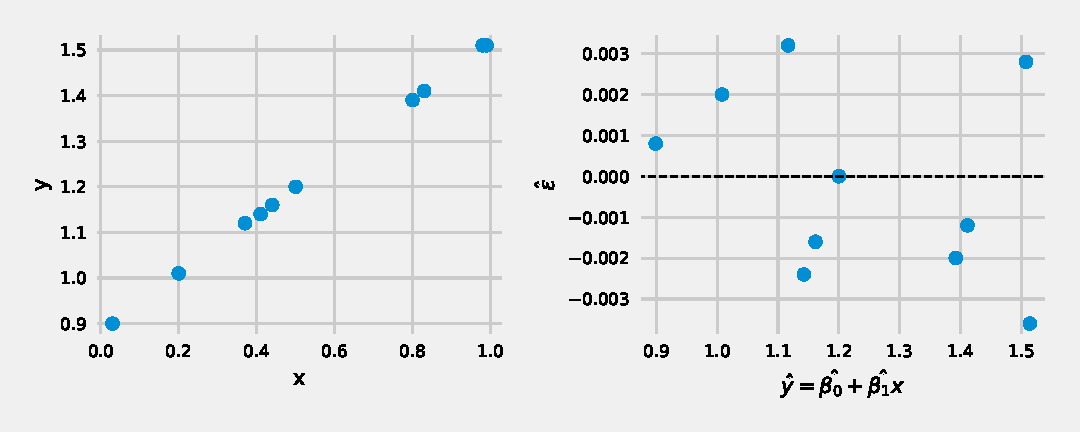
\includegraphics[width=\textwidth]{chapters/chapter7/ch6_residuals_vs_fitted.pdf}
    \caption{(Left) Scatter plot of $(x,y)$ pairs from the above dataset.
    (Right) Scatterplot of residuals versus fitted values. \label{fig.residualsDiag}}
\end{figure}

We see from the plot of $x$ vs $y$ that the relationship between $x$ and $y$ looks linear. In addition, the scatter plot of the fitted values versus residuals also looks like the residuals show not particular pattern and are centered around zero for all fitted values.

\subsubsection{Equal variance}

A plot of fitted values versus residuals can also be used to assess whether the assumption that the error $(\epsilon)$ is distributed $\mathcal{N}(0,\sigma^{2})$ according to a normal distribution with \textbf{the same variance for all values of $x$}.
This assumption is often called the equal variances assumption.

Below we generated 100 $(x,y)$ pairs of observed data points. 
We estimated our parameter values~(more on this later) and then computed fitted values and residuals. 
Again we plotted a scatterplot of $x$ vs $y$ and a plot of fitted values vs residuals.
We see from the residuals vs fitted values that it appears that the residuals move further away from zero as $x$ values increase.
This indicates that the \textbf{equal variances} assumption may not best describe our data.

\begin{figure}
    \centering
    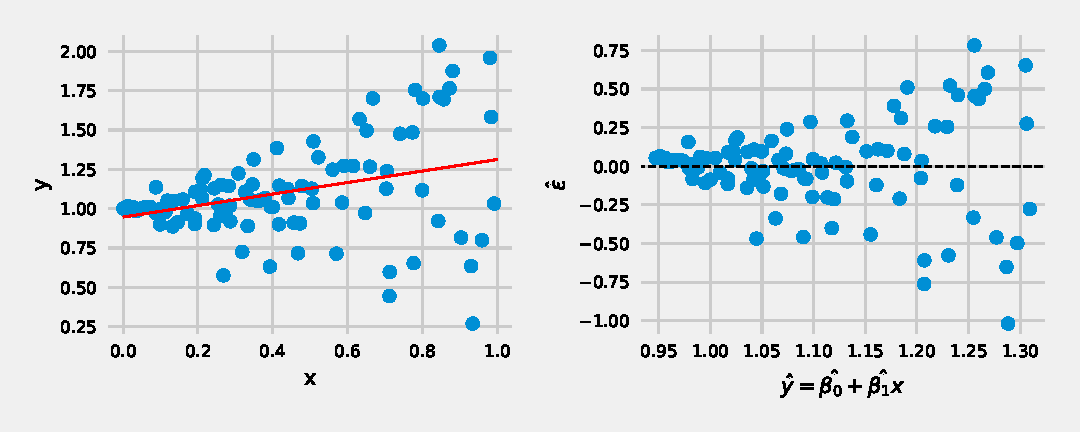
\includegraphics[width=\textwidth]{chapters/chapter7/ch6_residuals_vs_fitted__extravar.pdf}
    \caption{(Left) Scatter plot of 100 $(x,y)$ pairs from the above dataset with the line (red) $\hat{\mathbb{E}(Y|x)} = \hat{\beta_{0}} + \hat{\beta_{1}}x$.
    (Right) Scatterplot of residuals versus fitted values. \label{fig.residualsDiag}}
\end{figure}

\subsection{Independence}

The independence between data points $d_{i} = (x_{i}, y_{i})$ and $d_{j} = (x_{j}, y_{j})$ for any $(i,j)$ can be tested with a sequence vs residual plot. 
For this plot we graph residuals versus a variable that indicates when in time the data was collected. 
For example, we may decide to plot the time the data point was collected vs residual, or we can rank the data by the time it was collected and plot the rank vs residual.
For single covariate linear regression, we expect that there does not exist a relationship between when the data was collected and the residuals.
We assume that errors $\epsilon$ are independent from one another.
If there is a relationship between when the data was collected and residuals then this may indicate the data points are not independent.

\begin{figure}
    \centering
    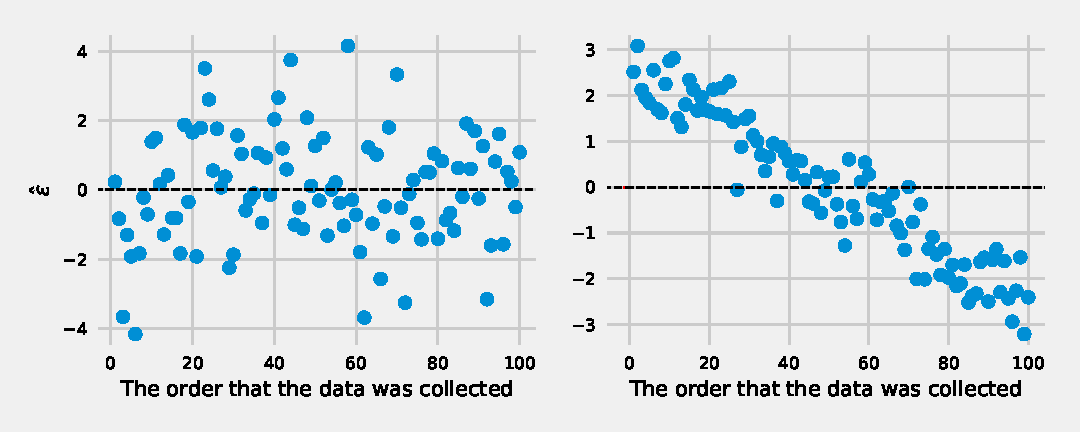
\includegraphics[width=\textwidth]{chapters/chapter7/ch6_residuals_vs_sequence.pdf}
    \caption{(Left) Scatter plot of 100 $(\text{order},\hat{\epsilon})$ pairs from a dataset where data was generated independently. 
    (Right) Scatterplot of the order that the data was collected versus residuals for data that was generated dependently. \label{fig.residualsDiag}}
\end{figure}


\section{Sums of squares}

Up until this point we assumed that we can compute estimates for $\beta_{0}$ and for $\beta_{1}$, but we have not yet discussed methods to compute estimates for these parameters. 
The first method we will explore is called \textbf{minimizing the sums of squares} or is often also called \textbf{least squares}.

Given a dataset $\mathcal{D} = \{ (x_{1},y_{1}), (x_{2},y_{2}), \cdots (x_{n},y_{n}) \}$ and a single covariate regression model $Y_{i} = \mu(x) + \epsilon$ where $\epsilon \sim \mathcal{N}(0,\sigma^{2})$, the least squares estimates for $\beta_{0}$ and $\beta_{1}$ are the values that minimize 
\begin{align}
    SS(\beta_{0}, \beta_{1}) = \sum_{i=1}^{N} \left[ y_{i} - \left(\beta_{0} + \beta_{1}x_{i} \right)  \right]^{2}
\end{align}
The function $SS(\beta_{0}, \beta_{1})$ is called the "sums of squares" function.
To minimize $SS(\beta_{0}, \beta_{1})$ we will
\begin{enumerate}
    \item Treat $\beta_{1}$ as a constant, treat $\beta_{0}$ as a variable, take the derivative and set that equation to zero. 
    \item Treat $\beta_{0}$ as a constant, treat $\beta_{1}$ as a variable, take the derivative and set that equation to zero. 
    \item Solve the above two equations for $\beta_{0}$ and $\beta_{1}$.
\end{enumerate}

\subsection{ $\beta_{0}$ as the variable and $\beta_{1}$ as a constant}

Because the SS function is a sum of similar terms, we can compute the derivative for one term and then add each term together. 

\begin{align}
    SS(\beta_{0})' &= \left\{ \sum_{i=1}^{N} \left[ y_{i} - \left(\beta_{0} + \beta_{1}x_{i} \right)  \right]^{2} \right \}' \\
    &=  \sum_{i=1}^{N} \left\{ \left[ y_{i} - \left(\beta_{0} + \beta_{1}x_{i} \right)   \right]^{2}\right \}
\end{align}

The goal then is to compute the derivative of 
\begin{align}
    SS(\beta_{0}) = \left[ y_{i} - \left(\beta_{0} + \beta_{1}x_{i} \right)  \right]^{2}
\end{align}
We will need to use the chain rule
\begin{align}
    SS(\beta_{0}) &= \left[ h(\beta_{0}) \right]^{2} \\ 
    h(\beta_{0}) &= y_{i} - \left(\beta_{0} + \beta_{1}x_{i} \right) \\
\end{align}

The derivative of 
\begin{align}
    SS(\beta_{0}) &= \left[ h(\beta_{0}) \right]^{2} \\
\end{align}
is 
\begin{align}
    SS(\beta_{0}) &= 2\left[ h(\beta_{0}) \right] \\
\end{align} and the derivative of 
\begin{align}
    h(\beta_{0}) &= y_{i} - \left(\beta_{0} + \beta_{1}x_{i} \right) \\
\end{align}
is 
\begin{align}
    h(\beta_{0})' &= - 1,
\end{align}
and so the derivative of $SS(\beta_{0})$ is 
\begin{align}
    SS(\beta_{0})' &= \sum_{i=1}^{N} 2\left[ h(\beta_{0}) \right] \times (-1) \\ 
                   &= \sum_{i=1}^{N} -2\left[y_{i} - \left(\beta_{0} + \beta_{1}x_{i} \right) \right]
\end{align}

We can set this equation equal to zero and solve for $\beta_{0}$ to find the least squares estimate for $\beta_{0}$
\begin{align}
    \sum_{i=1}^{N} -2\left[y_{i} - \left(\beta_{0} + \beta_{1}x_{i} \right) \right] &=0 \\ 
    \sum_{i=1}^{N} \left[y_{i} - \left(\beta_{0} + \beta_{1}x_{i} \right) \right] &=0 \\
    \sum_{i=1}^{N} y_{i} - \sum_{i=1}^{N} \beta_{0} -\sum_{i=1}^{N} \beta_{1}x_{i}  &=0 \\
    \sum_{i=1}^{N} y_{i} - N \beta_{0} -\sum_{i=1}^{N} \beta_{1}x_{i}  &=0 \\
    \sum_{i=1}^{N} y_{i}  -\sum_{i=1}^{N} \beta_{1}x_{i}  &= N \beta_{0} \\
    \sum_{i=1}^{N} y_{i}  - \beta_{1}\sum_{i=1}^{N} x_{i}  &= N \beta_{0} \\
    \frac{\sum_{i=1}^{N} y_{i}}{N}  - \beta_{1}\frac{\sum_{i=1}^{N}x_{i}}{N}  &=  \beta_{0}\\
    \bar{y} - \beta_{1}\bar{x}  &=  \beta_{0}
\end{align}

The \textbf{least squares estimate for $\beta_{0}$} is 
\begin{align}
    \hat{\beta_{0}}_{\text{SS}} = \bar{y} - \beta_{1} \bar{x}
\end{align}

\subsection{ $\beta_{1}$ as the variable and $\beta_{0}$ as a constant}

Lets take the same approach for computing an estimate for $\beta_{1}$.

\begin{align}
    SS(\beta_{1})' &= \left\{ \sum_{i=1}^{N} \left[ y_{i} - \left(\beta_{0} + \beta_{1}x_{i} \right)  \right]^{2} \right \}' \\
    &=  \sum_{i=1}^{N} \left\{ \left[ y_{i} - \left(\beta_{0} + \beta_{1}x_{i} \right)   \right]^{2}\right \}
\end{align}

The goal then is to compute the derivative of 
\begin{align}
    SS(\beta_{1}) = \left[ y_{i} - \left(\beta_{0} + \beta_{1}x_{i} \right)  \right]^{2}
\end{align}
We will need to use the chain rule
\begin{align}
    SS(\beta_{1}) &= \left[ h(\beta_{1}) \right]^{2} \\ 
    h(\beta_{1}) &= y_{i} - \left(\beta_{0} + \beta_{1}x_{i} \right)
\end{align}

The derivative of 
\begin{align}
    SS(\beta_{1}) &= \left[ h(\beta_{1}) \right]^{2}
\end{align}
is 
\begin{align}
    SS(\beta_{1}) &= 2\left[ h(\beta_{1}) \right] 
\end{align} and the derivative of 
\begin{align}
    h(\beta_{1}) &= y_{i} - \left(\beta_{0} + \beta_{1}x_{i} \right) 
\end{align}
is 
\begin{align}
    h(\beta_{0})' &= -x_{i},
\end{align}
and so the derivative of $SS(\beta_{1})$ is 
\begin{align}
    SS(\beta_{1})' &= \sum_{i=1}^{N} 2\left[ h(\beta_{1}) \right] \times (-x_{i}) \\ 
                   &= \sum_{i=1}^{N} -2x_{i}\left[y_{i} - \left(\beta_{0} + \beta_{1}x_{i} \right) \right]
\end{align}

We can set this equation equal to zero and solve for $\beta_{1}$ to find the least squares estimate for $\beta_{1}$
\begin{align}
    \sum_{i=1}^{N} -2x_{i}\left[y_{i} - \left(\beta_{0} + \beta_{1}x_{i} \right) \right] &= 0\\
    \sum_{i=1}^{N} -x_{i}\left[y_{i} - \left(\beta_{0} + \beta_{1}x_{i} \right) \right] &= 0\\
    \sum_{i=1}^{N} -x_{i} y_{i} + x_{i}\beta_{0} + \beta_{1}x^{2}_{i} &= 0\\
    \sum_{i=1}^{N} -x_{i} y_{i} + \beta_{0} \sum_{i=1}^{N} x_{i} + \beta_{1} \sum_{i=1}^{N} x^{2}_{i} &= 0\\
    \beta_{1} \sum_{i=1}^{N} x^{2}_{i} &= \sum_{i=1}^{N} x_{i} y_{i} - \beta_{0} \sum_{i=1}^{N} x_{i} \\
\end{align}

\subsection{Solving for $\beta_{0}$ and $\beta_{1}$}
At this point we have two equations and two unknowns:
\begin{align}
    \beta_{0} &= \bar{y} - \beta_{1} \bar{x} \\ 
     \beta_{1} \sum_{i=1}^{N} x^{2}_{i} &= \sum_{i=1}^{N} x_{i} y_{i} - \beta_{0} \sum_{i=1}^{N} x_{i} \\
\end{align}

We can solve the above equations and find that the least squares estimates for $\beta_{0}$ and for $\beta_{1}$ are

\begin{align}
    \hat{\beta_{1}} &= \frac{ \sum_{i=1}^{N} (x_{i} - \bar{x})(y_{i} - \bar{y})  }{ \sum_{i=1}^{N} (x_{i} - \bar{x})^{2} }\\
    \hat{\beta_{0}} &= \bar{y} - \hat{\beta_{1}} \bar{x} \\
\end{align}

\ex Suppose we collect the dataset 
\begin{table}[ht!]
    \centering
    \begin{tabular}{c|c}
        x & y \\
        \hline
        0.38 & 0.72\\
        0.04 & 1.00\\
        0.79 & 0.19\\
        0.48 & 0.69\\
        0.68 & 0.56\\
    \end{tabular}
\end{table}

We can compute the least squares estimates for $\beta_{0}$ and $\beta_{1}$ by following these steps:

\textbf{Compute $\bar{x}$ and $\bar{y}$}
\begin{align}
    \bar{x} = \frac{0.38 + 0.04 + 0.79 + 0.48 + 0.68}{5} = 0.47\\
    \bar{y} = \frac{0.72 + 1.00 + 0.19 + 0.69 + 0.56}{5} = 0.63\\
\end{align}

\clearpage
\textbf{Augment the above table with a column that computes $x_{i} - \bar{x}$ and $y_{i} - \bar{y}$}

\begin{table}[ht!]
    \centering
    \begin{tabular}{c|c|c|c }
        x & y & $(x_{i} - \bar{x})$ & $(y_{i} - \bar{y})$ \\
        \hline
        0.38 & 0.72 & -0.09 &  0.09\\
        0.04 & 1.00 & -0.43 &  0.37\\
        0.79 & 0.19 & 0.31  &  -0.44\\
        0.48 & 0.69 & 0.01  &  0.05 \\
        0.68 & 0.56 & 0.21. &  -0.07 \\
    \end{tabular}
\end{table}


\textbf{Add a column that computes  $(x_{i} - \bar{x})(y_{i} - \bar{y})$ and that computes $(x_{i} - \bar{x})^{2}$}

\begin{table}[ht!]
    \centering
    \begin{tabular}{c|c|c|c|c|c }
        x & y & $(x_{i} - \bar{x})$ & $(y_{i} - \bar{y})$ & $(x_{i} - \bar{x})(y_{i} - \bar{y})$ & $(x_{i} - \bar{x})^{2}$ \\
        \hline
        0.38 & 0.72 & -0.09 &  0.09  & -0.01 & 0.01 \\
        0.04 & 1.00 & -0.43 &  0.37  & -0.16 & 0.18 \\
        0.79 & 0.19 & 0.31  &  -0.44 & -0.14 & 0.10 \\
        0.48 & 0.69 & 0.01  &  0.05  & 0.00  & 0.0 \\
        0.68 & 0.56 & 0.21. &  -0.07 & -0.02 & 0.04 \\
    \end{tabular}
\end{table}

\textbf{Compute the sums of the last two columns and divide the second to last column by the last column to estimate $\beta_{1}$ }

\begin{align}
    \sum_{i=1}^{N} (x_{i} - \bar{x})(y_{i} - \bar{y}) &= -0.01 -0.16 - 0.14 + 0.00 - 0.02  = - 0.33 \\ 
    \sum_{i=1}^{N} (x_{i} - \bar{x})^{2} &= 0.01 + 0.18 + 0.10 + 0.0 + 0.04 = 0.33 \\ 
    \hat{\beta_{1}} &= -0.33 / 0.33 = -1
\end{align}

\textbf{Use your estimate for $\beta_{1}$ to estimate $\beta_{0}$}
\begin{align}
    \hat{\beta_{0}} &= \bar{y} - \hat{\beta_{1}} \bar{x} \\ 
    \hat{\beta_{0}} &= 0.63 - (-1)(0.47)  = 1.1
\end{align}



\section{Maximum likelihood estimates for $\beta_{0}$, $\beta_{1}$, and $\sigma^{2}$}

We must estimate three parameters for single covariate linear regression: $\beta_{0}, \beta_{1}, \sigma^{2}$.
We will take a maximum likelihood approach to estimate these three covariates in two steps.
Step one: compute the log-liklihod for a typical univariate normal distribution. Step two: convert this loglikelihood to single covariate linear regression.

Give a sample $\mathcal{D} = \{ (x_{1},y_{1}), (x_{2},y_{2}), (x_{3},y_{3}), \cdots, (x_{n},y_{n})\}$ assume that we model $Y$ as $Y_{i} \sim \mathcal{N}\left(\mu, \sigma^{2} \right)$ where $\mu$ does not depend on $x$ observations. 

Then the likelihood can be computed as 
\begin{align*}
    \ell ( \mu, \sigma^{2}) &= f(y_{1}) \cdot f(y_{2}) \cdot f(y_{3}) \cdots f(y_{n}) \\ 
    &= \frac{1}{\sqrt{2 \pi \sigma^{2} } } \exp \left[  \frac{1}{2 \sigma^{2}} \left (y_{1} - \mu \right)^{2} \right] \cdot \frac{1}{\sqrt{2 \pi \sigma^{2} } } \exp \left[  \frac{1}{2 \sigma^{2}} \left (y_{2} - \mu \right)^{2} \right] \\
    & \cdot \frac{1}{\sqrt{2 \pi \sigma^{2} } } \exp \left[  \frac{1}{2 \sigma^{2}} \left (y_{3} - \mu \right)^{2} \right] \cdots \frac{1}{\sqrt{2 \pi \sigma^{2} } } \exp \left[  \frac{1}{2 \sigma^{2}} \left (y_{n} - \mu \right)^{2} \right]
\end{align*}

Lets simplify this equation by computing the log likelihood. 
\begin{align*}
    \ell \ell ( \mu, \sigma^{2}) &= -\frac{1}{2} \log \left(2 \pi \sigma^{2}\right) - \left[  \frac{1}{2 \sigma^{2}} \left (y_{1} - \mu \right)^{2} \right] 
    -\frac{1}{2} \log \left(2 \pi \sigma^{2}\right) - \left[  \frac{1}{2 \sigma^{2}} \left (y_{2} - \mu \right)^{2} \right]\\
    &-\frac{1}{2} \log \left(2 \pi \sigma^{2}\right) - \left[  \frac{1}{2 \sigma^{2}} \left (y_{3} - \mu \right)^{2} \right]
    \cdots 
    -\frac{1}{2} \log \left(2 \pi \sigma^{2}\right) - \left[  \frac{1}{2 \sigma^{2}} \left (y_{n} - \mu \right)^{2} \right] \\
    &= \sum_{i=1}^{n} -\frac{1}{2} \log \left(2 \pi \sigma^{2}\right) - \left[  \frac{1}{2 \sigma^{2}} \left (y_{i} - \mu \right)^{2} \right] \\
    &= - \frac{N}{2} \log \left(2 \pi \sigma^{2}\right) - \sum_{i=1}^{n} \left[  \frac{1}{2 \sigma^{2}} \left (y_{i} - \mu \right)^{2} \right] \\
    &= - \frac{N}{2} \log \left(2 \pi \sigma^{2}\right) - \frac{1}{2 \sigma^{2}} \sum_{i=1}^{n} \left[   \left (y_{i} - \mu \right)^{2} \right] \\
\end{align*}

Our log likelihood is a function of two parameters. 
To maximize for $\mu$, we pretend that our log likelihood is a function of just $\mu$ and treat $\sigma^{2}$ as a constant. 
To maximize for $\sigma^{2}$, we pretend that our log likelihood is a function of $\sigma^{2}$ and treat $\mu$ as a constant.

The maximum likelihood estimate~(mle) for $\mu$ is 
\begin{align}
    \hat{\mu}_{\text{mle}} = \sum_{i=1}^{N} y_{i}  /  N 
\end{align}
and the mle for $\sigma^{2}$ is 
\begin{align}
    \hat{\sigma^{2}}_{\text{mle}} = \sum_{i=1}^{N} \frac{\left(y_{i} - \hat{\mu}_{\text{mle}} \right)^{2}}{N} 
\end{align}

\section{Maximum likelihood estimate for $\sigma^{2}$ and the MSE}



\section{Homework}

\begin{enumerate}
    \item Are the following two datasets equal to one another? Why or why not? 
    \begin{align}
        \mathcal{D}_{1} = \{ (3,1),(0.1,10),(-1,1),(1,0) \}\\
        \mathcal{D}_{2} = \{(0.1,10), (1,0),(3,1),(-1,1) \}
    \end{align}
    
    \item  Suppose that you are asked to explore in a group of patients who have a family history of heard disease the relationship between the number of packs of cigarettes smoked by the patient and Creatine Kinase-MB (CK-MB), an enzyme found in heart muscle that when elevated indicates damage to the heart.
    CK-MB is a measurement that is at minimum 0.\\
    
    You're first thought is to fit a linear regression model of the form
    \begin{align}
        Y_{i}| x_{i} \sim \mathcal{N}\left( \beta_{0} + \beta_{1} x_{i}, \sigma^{2} \right)
    \end{align}
    where $Y_{i}$ is a random variable that we assume generates CK-MB levels for patient $i$ and $x_{i}$ is the reported number of packs smoked per day. 
    
    \begin{enumerate}
        \item What is the support of a Normal distribution? Is this assumption reasonable to model CK-MB? 
        \item Suppose we collect data and estimate $\beta_{0}$ as $\hat{\beta_{0}} = 200$ and $\hat{\beta_{1}} = 10$. 
        How would you interpret $\hat{\beta_{0}}$?
    \end{enumerate}

    \item Assume that we decide to model a dataset $\mathcal{D} = ( (x_{1},y_{1}),(x_{2},y_{2}),\cdots,(x_{n},y_{n})  )$ as 
    \begin{align}
        Y_{i} | x_{i} \sim \mathcal{N}\left( \beta_{0} + \beta_{1} x_{i}, \sigma^{2} \right)
    \end{align}
    
    \begin{enumerate}
        \item Let $E = Y_{i} | x_{i} - (\beta_{0} + \beta_{1} x_{i})$. 
        What is the distribution of $E$? 
        \item Let $Z = \frac{Y_{i} - (\beta_{0} + \beta_{1} x_{i})}{\sigma}$. What is the distribution of $Z$?
    \end{enumerate}
    
    \item We assume that in linear regression 
    \begin{align}
        Y_{i} | x_{i} \sim \mathcal{N}\left( \beta_{0} + \beta_{1} x_{i}, \sigma^{2} \right)
    \end{align}
    the variable $x_{i}$ is generated randomly. Why or why not?
    
    \item Suppose that we decide to model $\mathcal{D} = ( y_{1}, y_{2}, y_{3}, \cdots, y_{n})$ as $Y_{i} \sim \mathcal{N}\left(\mu,\sigma^{2} \right)$. 
    The loglikelihood function for the normal distribution is
    \begin{align}
         \ell \ell(\mu, \sigma^{2}) = - \frac{N}{2} \log \left(2 \pi \sigma^{2}\right) - \frac{1}{2 \sigma^{2}} \sum_{i=1}^{n} \left[   \left (y_{i} - \mu \right)^{2} \right]
    \end{align}
    \begin{enumerate}
        \item Please compute the mle for $\mu$ by computing the derivative, treating $\mu$ as a variable and $\sigma^{2}$ as a constant 
        \item Please compute the mle for $\sigma^{2}$ by computing the derivative, treating $\sigma^{2}$ as a variable and $\mu$ as a constant 
    \end{enumerate}
    
    
    \item Please compute for all values of $q$ the quantities $\mathbb{E}(R|q)$ and $\mathbb{V}(R|q)$
    \begin{table}[ht!]
        \centering
        \begin{tabular}{c|ccc}
             & q= -1 & q=0 & q=1  \\
             \hline
        r=-2 & 0.10  & 0.90 & 0.25 \\
        r=-1 & 0.57  & 0.05 & 0.25 \\
        r= 0 & 0.13  & 0.05 & 0.25 \\
        r= 1 & 0.20  & 0.00 & 0.25 \\
        \end{tabular}
    \end{table}
    \item For the above table, why do the columns sum to the value one but the rows do not?
    
    \item Suppose we collected the following dataset
    \begin{table}[ht!]
        \centering
        \begin{tabular}{c|c}
            x & y \\
            \hline
            -2  & -2.83  \\ 
            0   &  -0.78 \\ 
            2   &  2.83  \\ 
            1   &  0.74  \\ 
            0   &  0.67  \\ 
            1   &  2.48  \\ 
            2   &  2.52  \\ 
            3   &  3.75  \\ 
            -1  &  -0.91 \\ 
            -2  &  -1.42 \\ 
        \end{tabular}
    \end{table}
    \begin{enumerate}
        \item Please compute all fitted values
        \item Please compute all residuals
        \item Plot residuals vs fitted values
        \item Plot residuals vs the order that the data was collected where the top row was the first collected data point and the last row in the table was the 10th data point collected. 
        \item Does the linearity assumption appear to hold for this dataset? Why or why not?
        \item Does the equal variances assumption appear to hold? Why or why not?
    \end{enumerate}
    
    
    
    \item Suppose we build a scatter plot of the relationship between observations of a variable $x$ and variable $y$. 
    We decide to fit a linear regression and add to the plot $\mathbb{E}(Y|x)$. 
    
    \begin{figure}[ht!]
        \centering
        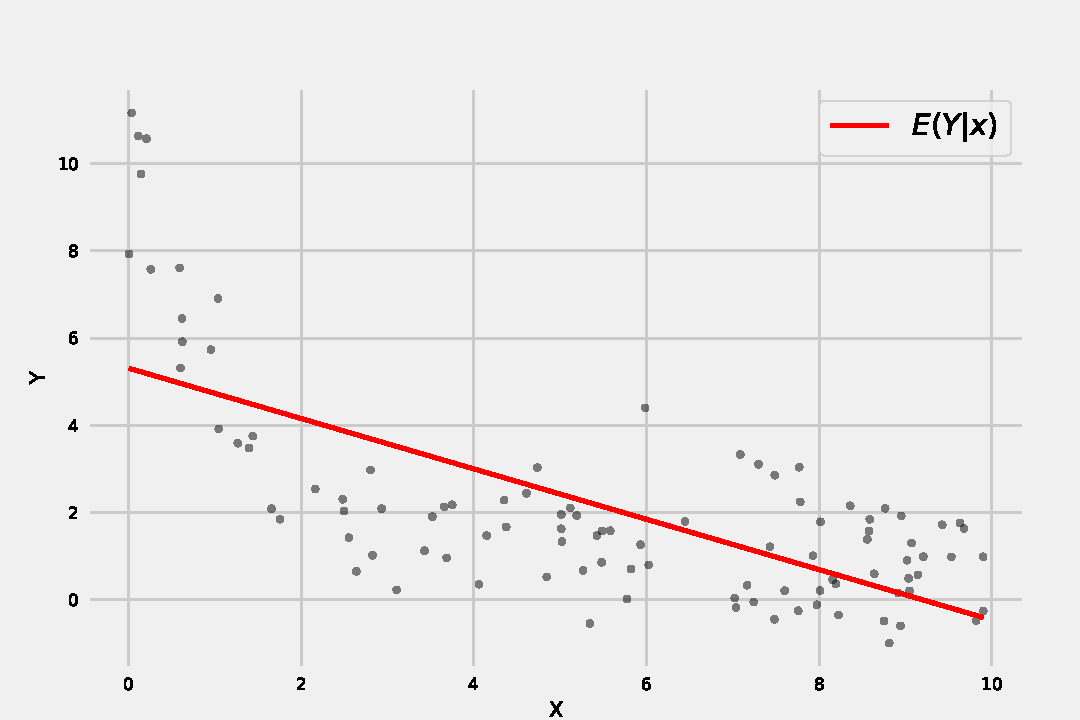
\includegraphics{chapters/chapter7/nonlinear_relationship.pdf}
    \end{figure}
    
    Please sketch what you would expect the residual vs fitted value plot to look like.
    
    \item Suppose that you fit a linear regression model and compute the residuals.
    As the residuals move closer to the line $\mathbb{E}(Y|x)$ will your estimate of $\sigma^{2}$ be smaller or larger? Why?  
    
    \item A linear regression is fit to a dataset where we collected the number of lbs of sugar an undergraduate student consumes during a week in the Fall semester and their H1Ac level.
    We estimate our parameters and find that $\hat{\beta_{0}} = 2$ and $\hat{\beta_{1}} = 10$. It may (or may not) be more reasonable to express the change in H1Ac not in increments of 1lb but instead in increments of 1 ounce.
    Please reexpress the estimated change in H1Ac in ounces of sugar consumed.  
    
    \item Will different parameter estimates lead to different diagnostic plots? Why or why not?
    
    \item The loglikelihood for single covariate regression is 
    \begin{align}
        \ell \ell (\beta_{0}, \beta_{1}, \sigma^{2}) = - \frac{N}{2} \log \left(2 \pi \sigma^{2}\right) - \frac{1}{2 \sigma^{2}} \sum_{i=1}^{n} \left\{   \left \left[y_{i} - (\beta_{0} + \beta_{1}x_{i}) \right]^{2} \right\}
    \end{align}
    We will compute the maximum likelihood estimate for $\beta_{1}$ in a series of steps.
    \begin{enumerate}
        \item Are only variable of interest is $\beta_{1}$. The paramters $\beta_{0}$ and $\sigma^{2}$ can be thought of as constants. Remove any terms in the loglikelihood that are constants. Call this new function $g$
        
        \item Compute the derivative of $g(\beta_{1})$, treating $\beta_{1}$ as a variable.
        
        \item Set $g'(\beta_{1}) = 0$ and solve for $\beta_{1}$ 
        
    \end{enumerate}
    
    \item We saw that we can compute estimates for $\beta_{0}$ and $\beta_{1}$ by minimizing the sums of squares or by maximum likelihood. 
    Please describe how the sums of squares estimates and maximum likelihood estimates are related and why they are related.
    
    \item Why can minimizing the sums of squares function $SS(\beta_{0}, \beta_{1})$ be interpreted as finding the values $(\beta_{0}), \beta_{1}$ that minimize \textbf{the sum} of squared residuals? Why can this minimizatoin be interpreted as minimizing \textbf{the mean} of squared residuals?
    
    \item Suppose we collect the dataset
    \begin{table}[ht!]
        \centering
        \begin{tabular}{c|c}
            x & y \\
            \hline
            -0.72 &  -3.33\\
            -0.78 &  -2.15\\
            -0.69 &  -1.94\\
            -0.12 &  -0.68\\
             0.70 &  0.20\\
            -0.30 &  -0.47\\
            -0.15 &  -2.20\\
            -0.71 &  -1.37\\
            -0.49 &  -1.16\\
             0.92 &  1.77\\
        \end{tabular}
    \end{table}
    \begin{enumerate}
        \item Compute the maximum likelihood estimate for $\beta_{0}$
        \item Compute the maximum likelihood estimate for $\beta_{1}$
        \item Compute the maximum likelihood estimate for $\sigma^{2}$
    \end{enumerate}
    
    \item Suppose we collect the dataset
    \begin{table}[ht!]
        \centering
        \begin{tabular}{c|c}
            x & y \\
            \hline
            -0.49 &  -2.20\\
            -0.55 &  -1.01\\
            -0.46 &  -0.80\\
             0.11 &  0.46\\
             0.93 &  1.34\\
            -0.07 &  0.66\\
             0.08 &  -1.07\\
            -0.48 &  -0.24\\
            -0.26 &  -0.03\\
             1.15 &  2.90\\
        \end{tabular}
    \end{table}
    \begin{enumerate}
        \item Compute the maximum likelihood estimate for $\beta_{0}$
        \item Compute the maximum likelihood estimate for $\beta_{1}$
        \item Compute the maximum likelihood estimate for $\sigma^{2}$
    \end{enumerate}
    
\end{enumerate}







\part{Algorithms lab}


 \chapterauthor{thomas mcandrew, david braun}{Lehigh University}
%\chapterauthor{Second Author}{Second Author Affiliation}
\chapter{Laboratory 01}
\hspace{1mm}
    \hypertarget{jupyter-notebooks}{%
\section{Jupyter Notebooks}\label{jupyter-notebooks}}

All of our lab work will take place in Jupyter Notebooks. Jupyter
Notebooks are a tool for organizing textual descriptions of work and
computer programs. The goal is to produce one document to communicate a
set of scientific ideas and allow another to understand exactly how you
arrived at yoru conclusions.

Jupyter has some important buttons.

\hypertarget{file}{%
\subsection{File}\label{file}}

\hypertarget{a-new-notebook}{%
\subsubsection{A new notebook}\label{a-new-notebook}}

Under file-\textgreater New-\textgreater Notebook you can create a new
notebook. When asked to ``Select Kernel'' click on the drop down menu
and select ``R''

\begin{figure}
\centering
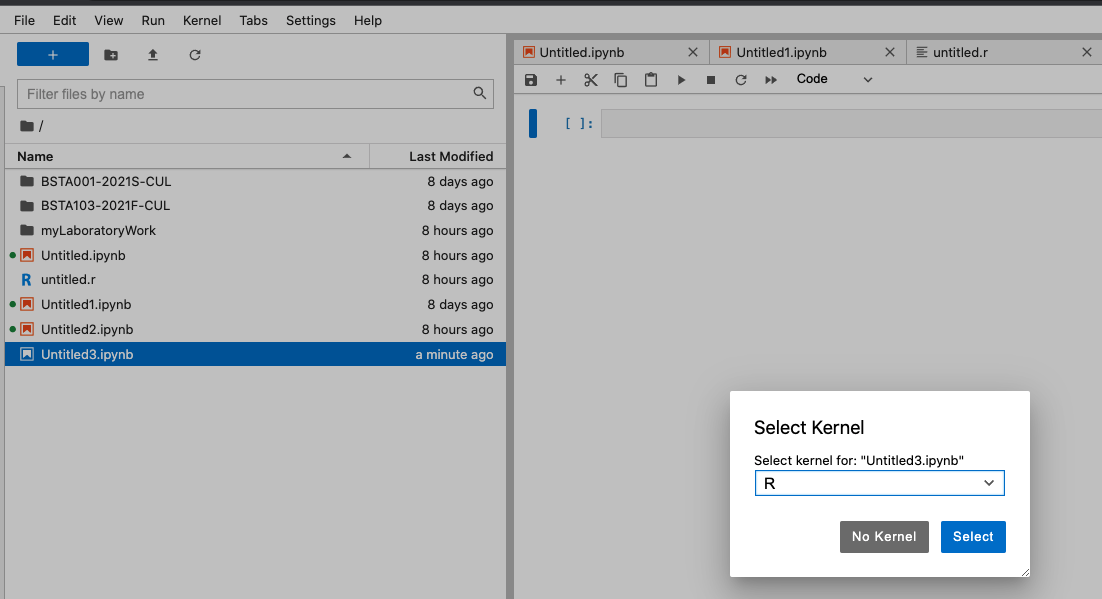
\includegraphics{chapters/chapter1/kernelselect}
\caption{kernelselect.png}
\end{figure}

\hypertarget{the-notebook}{%
\subsubsection{The notebook}\label{the-notebook}}

A notebook is a collection of cells. A \textbf{cell} is a container that
can hold text or computer code. Cells in Jupyter looks like gray
rectangles. There are three cell types in Jupyter: (i) Code, (ii)
Markdown, and (iii) Raw. The two that we will focus on are Code and
Markdown.

The ``Code'' cell holds computer code that the R kernel (see below about
a kernel) can use to compute. We may want to import data, run a
statistical analysis, and output results. This is for the ``Code'' cell.

``Markdown'' is itself a special language that a Jupyter Notebook
interprets as text. The ``Markdown'' cell is most useful for write ups,
descriptions of a Code cell above or below, or scientific conclusions,
comments, and thoughts. When you need to write, think Markdown.

\hypertarget{save-your-work}{%
\subsubsection{Save your work}\label{save-your-work}}

You can always save your work, and should do so often, by clicking File
-\textgreater{} Save Notebook.

\hypertarget{export-for-submission}{%
\subsubsection{Export for submission}\label{export-for-submission}}

In class, we will ask that you submit your work on Coursesite as a
\textbf{PDF}. Work in another format will not be accepted. To export
your notebook as a PDF, choose File-\textgreater Save and Export
Notebook As-\textgreater PDF 

\begin{figure}
    \centering
    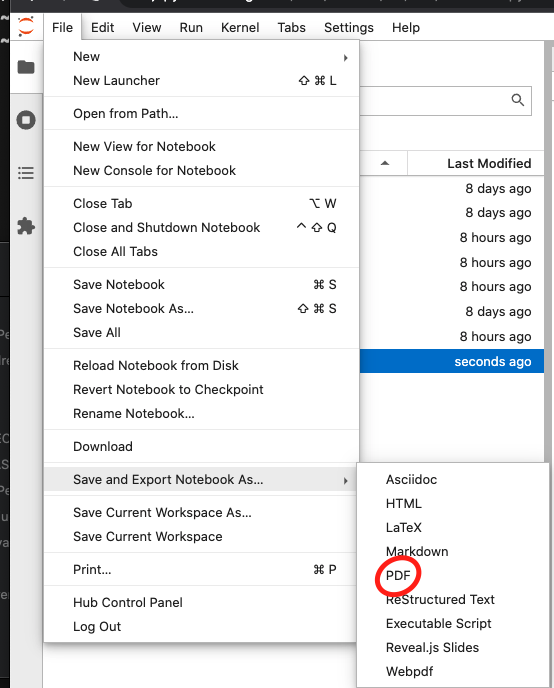
\includegraphics{chapters/chapter1/savepdf.png}
    \caption{Caption}
    \label{fig:my_label}
\end{figure}


After you
click PDF, a PDF file will be created and saved in a ``Downloads''
folder on your local machine. Make sure the PDF file contains (1) Your
first and surname, the date, and a descriptive title.

\hypertarget{kernel}{%
\subsection{Kernel}\label{kernel}}

The kernel is the component that executes code inside your notebook. No
kernel, no running code.

Over the course, you may find that your notebook has disconnected or
otherwise will no longer execute the code you wrote. Most often, the
kernel has stopped. To restart you kernel select
Kernel-\textgreater Restart Kernel.

    \hypertarget{programming-and-r}{%
\section{Programming and R}\label{programming-and-r}}

The R programming language, while not explictly written for statistics,
has a long history as a tool for data analysis, statistics, machine
learning, and data science. R supports all of the main paradigms in
computing and you will be able to transfer what you learn in R to other
programming languages without much difficulty.

Programming is difficult. Like any skill, programming take time to
master. Error messages will be commonplace, you will find it difficult
to ask the computer to calculate what you want. You will be frustrate
and that is ok. Over time you will learn to read the error messages,
code will flow more easily. The most important part of programming is
daily practice.

When we \textbf{execute} code, we ask the computer to translate what we
wrote into binary and return a set of results that may or may not be
stored in memory. In the Jupyter environment we execute code by pressing
``Run'' or by using the shortcut ``Shift+Enter''.

    \hypertarget{arithmetic}{%
\section{Arithmetic}\label{arithmetic}}

R supports all standard artithmetic calculations. Lets ``Run'' our first
computation.

R can interpret addition

    \begin{tcolorbox}[breakable, size=fbox, boxrule=1pt, pad at break*=1mm,colback=cellbackground, colframe=cellborder]
\prompt{In}{incolor}{100}{\boxspacing}
\begin{Verbatim}[commandchars=\\\{\}]
\PY{l+m}{2}\PY{l+m}{+2}
\end{Verbatim}
\end{tcolorbox}

    4

    
    Subtraction

    \begin{tcolorbox}[breakable, size=fbox, boxrule=1pt, pad at break*=1mm,colback=cellbackground, colframe=cellborder]
\prompt{In}{incolor}{101}{\boxspacing}
\begin{Verbatim}[commandchars=\\\{\}]
\PY{l+m}{9}\PY{l+m}{\PYZhy{}3}
\end{Verbatim}
\end{tcolorbox}

    6

    
    Division

    \begin{tcolorbox}[breakable, size=fbox, boxrule=1pt, pad at break*=1mm,colback=cellbackground, colframe=cellborder]
\prompt{In}{incolor}{102}{\boxspacing}
\begin{Verbatim}[commandchars=\\\{\}]
\PY{l+m}{3}\PY{o}{/}\PY{l+m}{4}
\end{Verbatim}
\end{tcolorbox}

    0.75

    
    multiplication

    \begin{tcolorbox}[breakable, size=fbox, boxrule=1pt, pad at break*=1mm,colback=cellbackground, colframe=cellborder]
\prompt{In}{incolor}{103}{\boxspacing}
\begin{Verbatim}[commandchars=\\\{\}]
\PY{l+m}{4}\PY{o}{*}\PY{l+m}{4}
\end{Verbatim}
\end{tcolorbox}

    16

    
    and exponentiation

    \begin{tcolorbox}[breakable, size=fbox, boxrule=1pt, pad at break*=1mm,colback=cellbackground, colframe=cellborder]
\prompt{In}{incolor}{104}{\boxspacing}
\begin{Verbatim}[commandchars=\\\{\}]
\PY{l+m}{3}\PY{o}{\PYZca{}}\PY{l+m}{9}
\end{Verbatim}
\end{tcolorbox}

    19683

    
    As expected, we can compute more difficult arithemetic expressions.

    \begin{tcolorbox}[breakable, size=fbox, boxrule=1pt, pad at break*=1mm,colback=cellbackground, colframe=cellborder]
\prompt{In}{incolor}{105}{\boxspacing}
\begin{Verbatim}[commandchars=\\\{\}]
\PY{p}{(}\PY{l+m}{2}\PY{o}{\PYZca{}}\PY{l+m}{4}\PY{p}{)}\PY{l+m}{+3}\PY{o}{/}\PY{l+m}{2} \PY{o}{\PYZhy{}} \PY{l+m}{1}
\end{Verbatim}
\end{tcolorbox}

    16.5

    
    \hypertarget{vectors}{%
\section{Vectors}\label{vectors}}

The \textbf{vector} is the fundemental object in R.

A mathematical vector is an ordered list of numbers. They are denoted by
a sequence of numbers surrounded by square brackets.

\begin{align}
    v = \begin{bmatrix}
         1 \\
         2 \\
         3 \\
        \end{bmatrix}
\end{align} Above, the vector \textbf{v} is a vector of length 3 and
contains, in order, the values 1, 2, and 3.

In R, vectors are goven a name and stored in the computer in one of two
ways: (i) using the \textbf{c()} operator or (ii) using the assign
function.

\hypertarget{assignment}{%
\subsection{Assignment}\label{assignment}}

\hypertarget{c}{%
\subsubsection{c()}\label{c}}

We can store a vector named v with the values 1,2,3 in R as follows

    \begin{tcolorbox}[breakable, size=fbox, boxrule=1pt, pad at break*=1mm,colback=cellbackground, colframe=cellborder]
\prompt{In}{incolor}{106}{\boxspacing}
\begin{Verbatim}[commandchars=\\\{\}]
\PY{n}{v} \PY{o}{=} \PY{n+nf}{c}\PY{p}{(}\PY{l+m}{1}\PY{p}{,}\PY{l+m}{2}\PY{p}{,}\PY{l+m}{3}\PY{p}{)}
\end{Verbatim}
\end{tcolorbox}

    \hypertarget{assign}{%
\subsubsection{assign}\label{assign}}

We can also use the assign function to store a vector, named q, with the
values 3,2,1 as follows

    \begin{tcolorbox}[breakable, size=fbox, boxrule=1pt, pad at break*=1mm,colback=cellbackground, colframe=cellborder]
\prompt{In}{incolor}{107}{\boxspacing}
\begin{Verbatim}[commandchars=\\\{\}]
\PY{n+nf}{assign}\PY{p}{(}\PY{l+s}{\PYZdq{}}\PY{l+s}{q\PYZdq{}}\PY{p}{,}\PY{n+nf}{c}\PY{p}{(}\PY{l+m}{3}\PY{p}{,}\PY{l+m}{2}\PY{p}{,}\PY{l+m}{1}\PY{p}{)}\PY{p}{)}
\end{Verbatim}
\end{tcolorbox}

    \hypertarget{equals}{%
\subsubsection{equals}\label{equals}}

The equals sign \textbf{does not} represent two objects are equal to one
another. The equals sign in compiuter programming stands for ``assign''.

When we write \texttt{v\ =\ c(1,2,3)}, this is understood as ``we assign
the variable v to the vector (1,2,3). As an example, lets create a
vector \texttt{(4,5,6)} names \texttt{x} and then assign the variable
\texttt{y} to be the same as \texttt{x}

    \begin{tcolorbox}[breakable, size=fbox, boxrule=1pt, pad at break*=1mm,colback=cellbackground, colframe=cellborder]
\prompt{In}{incolor}{108}{\boxspacing}
\begin{Verbatim}[commandchars=\\\{\}]
\PY{n}{x} \PY{o}{=} \PY{n+nf}{c}\PY{p}{(}\PY{l+m}{4}\PY{p}{,}\PY{l+m}{5}\PY{p}{,}\PY{l+m}{6}\PY{p}{)}
\PY{n}{y} \PY{o}{=} \PY{n}{x}
\end{Verbatim}
\end{tcolorbox}

    The last line above does not ask whether or not \texttt{x} is the same
as \texttt{y}. Instead, this line assigns the variable \texttt{y} to be
the same vecor as \texttt{x}.

    \hypertarget{print}{%
\section{Print}\label{print}}

When we created the vectors \textbf{v} and \textbf{q} ``nothing
happened''. Though the vector v and q were created and stored in the
computer, R does not display these on your screen by default. One way to
view any object in R is to print it.

You can print an object, \texttt{x}, R by writing \texttt{print(x)}

    \begin{tcolorbox}[breakable, size=fbox, boxrule=1pt, pad at break*=1mm,colback=cellbackground, colframe=cellborder]
\prompt{In}{incolor}{109}{\boxspacing}
\begin{Verbatim}[commandchars=\\\{\}]
\PY{n+nf}{print}\PY{p}{(}\PY{n}{v}\PY{p}{)}
\end{Verbatim}
\end{tcolorbox}

    \begin{Verbatim}[commandchars=\\\{\}]
[1] 1 2 3
    \end{Verbatim}

    \begin{tcolorbox}[breakable, size=fbox, boxrule=1pt, pad at break*=1mm,colback=cellbackground, colframe=cellborder]
\prompt{In}{incolor}{110}{\boxspacing}
\begin{Verbatim}[commandchars=\\\{\}]
\PY{n+nf}{print}\PY{p}{(}\PY{n}{q}\PY{p}{)}
\end{Verbatim}
\end{tcolorbox}

    \begin{Verbatim}[commandchars=\\\{\}]
[1] 3 2 1
    \end{Verbatim}

    \begin{tcolorbox}[breakable, size=fbox, boxrule=1pt, pad at break*=1mm,colback=cellbackground, colframe=cellborder]
\prompt{In}{incolor}{111}{\boxspacing}
\begin{Verbatim}[commandchars=\\\{\}]
\PY{n+nf}{print}\PY{p}{(}\PY{n}{x}\PY{p}{)}
\PY{n+nf}{print}\PY{p}{(}\PY{n}{y}\PY{p}{)}
\end{Verbatim}
\end{tcolorbox}

    \begin{Verbatim}[commandchars=\\\{\}]
[1] 4 5 6
[1] 4 5 6
    \end{Verbatim}

    \textbf{You do not need to print any object, ever}. Printing is not
necessary. You should use print to explore whether you programmed
something write or to communicate scientific results.

    \hypertarget{combining-vectors}{%
\section{Combining vectors}\label{combining-vectors}}

We can append one vector to another in R by using the c() operator.
Suppose we wish to combine the two vectors \begin{align}
    x = \begin{bmatrix}
        1\\
        2\\
        3
        \end{bmatrix}; \;
    z = \begin{bmatrix}
        -1\\
        0.2\\
        90
        \end{bmatrix}
\end{align}

into one vector

\begin{align}
    r = \begin{bmatrix}
        1\\
        2\\
        3\\
        -1\\
        0.2\\
        90
        \end{bmatrix}
\end{align}

Lets first create the vectors \texttt{x} and \texttt{z}

    \begin{tcolorbox}[breakable, size=fbox, boxrule=1pt, pad at break*=1mm,colback=cellbackground, colframe=cellborder]
\prompt{In}{incolor}{112}{\boxspacing}
\begin{Verbatim}[commandchars=\\\{\}]
\PY{n}{x} \PY{o}{=} \PY{n+nf}{c}\PY{p}{(}\PY{l+m}{1}\PY{p}{,}\PY{l+m}{2}\PY{p}{,}\PY{l+m}{3}\PY{p}{)}
\PY{n}{z} \PY{o}{=} \PY{n+nf}{c}\PY{p}{(}\PY{l+m}{\PYZhy{}1}\PY{p}{,}\PY{l+m}{0.2}\PY{p}{,}\PY{l+m}{90}\PY{p}{)}
\end{Verbatim}
\end{tcolorbox}

    Now we can create the vector \texttt{r}

    \begin{tcolorbox}[breakable, size=fbox, boxrule=1pt, pad at break*=1mm,colback=cellbackground, colframe=cellborder]
\prompt{In}{incolor}{113}{\boxspacing}
\begin{Verbatim}[commandchars=\\\{\}]
\PY{n}{r} \PY{o}{=} \PY{n+nf}{c}\PY{p}{(}\PY{n}{x}\PY{p}{,}\PY{n}{z}\PY{p}{)}
\end{Verbatim}
\end{tcolorbox}

    If we want to check our work, we can print out \texttt{r}.

    \begin{tcolorbox}[breakable, size=fbox, boxrule=1pt, pad at break*=1mm,colback=cellbackground, colframe=cellborder]
\prompt{In}{incolor}{114}{\boxspacing}
\begin{Verbatim}[commandchars=\\\{\}]
\PY{n+nf}{print}\PY{p}{(}\PY{n}{r}\PY{p}{)}
\end{Verbatim}
\end{tcolorbox}

    \begin{Verbatim}[commandchars=\\\{\}]
[1]  1.0  2.0  3.0 -1.0  0.2 90.0
    \end{Verbatim}

    \hypertarget{indexing-and-access}{%
\section{Indexing and access}\label{indexing-and-access}}

Vectors are useful for storing several different numbers. We can access
single elements, or several elements inside a vector by (i) naming the
vector we want to access, (ii) typing square brackets ``{[}{]}''.

\hypertarget{numeric-indexing}{%
\subsection{Numeric indexing}\label{numeric-indexing}}

If we want to access the 4th element in \texttt{r}, we can type

    \begin{tcolorbox}[breakable, size=fbox, boxrule=1pt, pad at break*=1mm,colback=cellbackground, colframe=cellborder]
\prompt{In}{incolor}{115}{\boxspacing}
\begin{Verbatim}[commandchars=\\\{\}]
\PY{n}{r}\PY{p}{[}\PY{l+m}{4}\PY{p}{]}
\end{Verbatim}
\end{tcolorbox}

    -1

    
    If we want to access, the 2nd, 4th, and then the first element of
\texttt{r} we can include in square brackets the vector
\texttt{c(2,4,1)}

    \begin{tcolorbox}[breakable, size=fbox, boxrule=1pt, pad at break*=1mm,colback=cellbackground, colframe=cellborder]
\prompt{In}{incolor}{116}{\boxspacing}
\begin{Verbatim}[commandchars=\\\{\}]
\PY{n}{r}\PY{p}{[}\PY{n+nf}{c}\PY{p}{(}\PY{l+m}{2}\PY{p}{,}\PY{l+m}{4}\PY{p}{,}\PY{l+m}{1}\PY{p}{)}\PY{p}{]}
\end{Verbatim}
\end{tcolorbox}

    \begin{enumerate*}
\item 2
\item -1
\item 1
\end{enumerate*}


    
    We can access the 1st,2nd, and 3rd elements in \texttt{r} using the
vector \texttt{c(1,2,3)}, however a shortcut is to use the
\textbf{colon} operator. The colon operator takes as input two integers
(a,b) separated by a colon (a:b) and expands to the vector
\texttt{c(a,a+1,a+2,a+3,...,b)}.

Watch

    \begin{tcolorbox}[breakable, size=fbox, boxrule=1pt, pad at break*=1mm,colback=cellbackground, colframe=cellborder]
\prompt{In}{incolor}{117}{\boxspacing}
\begin{Verbatim}[commandchars=\\\{\}]
\PY{n}{z} \PY{o}{=} \PY{l+m}{3}\PY{o}{:}\PY{l+m}{5}
\end{Verbatim}
\end{tcolorbox}

    \begin{tcolorbox}[breakable, size=fbox, boxrule=1pt, pad at break*=1mm,colback=cellbackground, colframe=cellborder]
\prompt{In}{incolor}{118}{\boxspacing}
\begin{Verbatim}[commandchars=\\\{\}]
\PY{n+nf}{print}\PY{p}{(}\PY{n}{z}\PY{p}{)}
\end{Verbatim}
\end{tcolorbox}

    \begin{Verbatim}[commandchars=\\\{\}]
[1] 3 4 5
    \end{Verbatim}

    The colon operator is useful for accessing items in a vector

    \begin{tcolorbox}[breakable, size=fbox, boxrule=1pt, pad at break*=1mm,colback=cellbackground, colframe=cellborder]
\prompt{In}{incolor}{119}{\boxspacing}
\begin{Verbatim}[commandchars=\\\{\}]
\PY{n}{r}\PY{p}{[}\PY{l+m}{2}\PY{o}{:}\PY{l+m}{5}\PY{p}{]}
\end{Verbatim}
\end{tcolorbox}

    \begin{enumerate*}
\item 2
\item 3
\item -1
\item 0.2
\end{enumerate*}


    
    The above is called \textbf{numeric indexing}. Numeric indexing is the
access of elements in an object (here a vector) by inputting a single
number, or vector of numbers. Indices are always integers. Fractional or
decimal numbers cannot be used as indices. Up until now we only used
\emph{positive} integers to access elements of a vector.

R also accepts negative integers as indices. Warning: R handles negative
indices different than the majority of other progamming languages. A
negative index in R standard for \textbf{exclude}.

For example, if we want to return all the elements of a vector
\texttt{q\ =\ c(1,4,6,10,0.5)} except for the 2nd element, we can write
\texttt{q{[}-2{]}}

    \begin{tcolorbox}[breakable, size=fbox, boxrule=1pt, pad at break*=1mm,colback=cellbackground, colframe=cellborder]
\prompt{In}{incolor}{120}{\boxspacing}
\begin{Verbatim}[commandchars=\\\{\}]
\PY{n}{q} \PY{o}{=} \PY{n+nf}{c}\PY{p}{(}\PY{l+m}{1}\PY{p}{,}\PY{l+m}{4}\PY{p}{,}\PY{l+m}{6}\PY{p}{,}\PY{l+m}{10}\PY{p}{,}\PY{l+m}{0.5}\PY{p}{)}
\PY{n}{q}\PY{p}{[}\PY{l+m}{\PYZhy{}2}\PY{p}{]}
\end{Verbatim}
\end{tcolorbox}

    \begin{enumerate*}
\item 1
\item 6
\item 10
\item 0.5
\end{enumerate*}


    
    \hypertarget{logical-vectors-and-logical-indexing}{%
\subsection{Logical vectors and logical
indexing}\label{logical-vectors-and-logical-indexing}}

\hypertarget{true-and-false}{%
\subsubsection{True and False}\label{true-and-false}}

R, like all programming languages, understands how to operate with
binary logic (aside: binary logic is not the only type. If interested,
google the tetralemma). True in R is represeted as the word
\texttt{TRUE} in all capitals. False in R is represented as the word
\texttt{FALSE} in all capitals. The symbols \texttt{TRUE} and
\texttt{FALSE} are reserved, special symbols in R. You cannot assign a
variable to \texttt{TRUE} or \texttt{FALSE}.

    \begin{tcolorbox}[breakable, size=fbox, boxrule=1pt, pad at break*=1mm,colback=cellbackground, colframe=cellborder]
\prompt{In}{incolor}{121}{\boxspacing}
\begin{Verbatim}[commandchars=\\\{\}]
\PY{k+kc}{TRUE}
\end{Verbatim}
\end{tcolorbox}

    TRUE

    
    \begin{tcolorbox}[breakable, size=fbox, boxrule=1pt, pad at break*=1mm,colback=cellbackground, colframe=cellborder]
\prompt{In}{incolor}{122}{\boxspacing}
\begin{Verbatim}[commandchars=\\\{\}]
\PY{k+kc}{FALSE}
\end{Verbatim}
\end{tcolorbox}

    FALSE

    
    \hypertarget{logical-comparisons}{%
\subsubsection{Logical comparisons}\label{logical-comparisons}}

R understand the following logical operators: - \texttt{\textgreater{}}
``Greater than'' - \texttt{\textgreater{}=} ``Greater than or equal to''
- \texttt{\textless{}} ``Less than'' - \texttt{\textless{}=} ``Less than
or equal to'' - \texttt{==} ``Is equal to'' - \texttt{!=} ``Not equal''
- \texttt{\textbar{}} ``OR'' - \texttt{\&} ``AND''

\hypertarget{logic}{%
\subsubsection{Logic}\label{logic}}

Logic is a method to evaluate statements, sometimes called propositions
as either True or False. The above symbols are used to evaluate
statements.

When you pose a proposition to R, such as \texttt{v\ \textgreater{}\ -1}
R will evaluate that propositon for each individual element in the
vector \texttt{v}. Lets create the vector \texttt{v\ =\ c(-10,10,4)} and
ask R to evaluate the proposition \texttt{v\textgreater{}-1}.

    \begin{tcolorbox}[breakable, size=fbox, boxrule=1pt, pad at break*=1mm,colback=cellbackground, colframe=cellborder]
\prompt{In}{incolor}{123}{\boxspacing}
\begin{Verbatim}[commandchars=\\\{\}]
\PY{n}{v} \PY{o}{=} \PY{n+nf}{c}\PY{p}{(}\PY{l+m}{\PYZhy{}10}\PY{p}{,}\PY{l+m}{10}\PY{p}{,}\PY{l+m}{4}\PY{p}{)}
\PY{n}{v} \PY{o}{\PYZgt{}} \PY{l+m}{\PYZhy{}1}
\end{Verbatim}
\end{tcolorbox}

    \begin{enumerate*}
\item FALSE
\item TRUE
\item TRUE
\end{enumerate*}


    
    We see that R returns a vector with the same numebr of elements as in v
containing the values TRUE or FALSE. A vector that contains values
TRUE/FALSE is called a \textbf{logical vector}. Like any other vector we
can store a logical vector.

    \begin{tcolorbox}[breakable, size=fbox, boxrule=1pt, pad at break*=1mm,colback=cellbackground, colframe=cellborder]
\prompt{In}{incolor}{124}{\boxspacing}
\begin{Verbatim}[commandchars=\\\{\}]
\PY{n}{log} \PY{o}{=} \PY{n}{v}\PY{o}{\PYZgt{}}\PY{l+m}{\PYZhy{}1}
\end{Verbatim}
\end{tcolorbox}

    \begin{tcolorbox}[breakable, size=fbox, boxrule=1pt, pad at break*=1mm,colback=cellbackground, colframe=cellborder]
\prompt{In}{incolor}{125}{\boxspacing}
\begin{Verbatim}[commandchars=\\\{\}]
\PY{n+nf}{print}\PY{p}{(}\PY{n}{log}\PY{p}{)}
\end{Verbatim}
\end{tcolorbox}

    \begin{Verbatim}[commandchars=\\\{\}]
[1] FALSE  TRUE  TRUE
    \end{Verbatim}

    \hypertarget{and-or-and-not}{%
\subsubsection{AND, OR, and NOT}\label{and-or-and-not}}

AND, OR, and NOT are \textbf{logical operators}, they allow us to
combine one or more propositions. Given two propositions \(p_{1}\) and
\(p_{2}\), the AND, OR, and NOT operator will evaluate to the following


\begin{table}[ht!]
    \centering
    \begin{tabular}{ccccc}
        \hline
        $p_{1}$ &$p_{2}$ &$p_{1}$ AND $p_{2}$ &$p_{1}$ OR $p_{2}$ &!$p_{1}$\\
        \hline \vspace{1mm}
        TRUE & TRUE & TRUE & TRUE & FALSE \\
        TRUE & FALSE & FALSE & TRUE & FALSE \\
        FALSE & TRUE & FALSE & TRUE & TRUE \\
        FALSE & FALSE & FALSE & FALSE & TRUE \\
    \hline
    \end{tabular}
    \caption{Caption}
    \label{tab:my_label}
\end{table}


Logical operators come in handy in \textbf{logical indexing}. When we
write \texttt{r{[}l{]}} where \texttt{l} is a logical vector, R will
return the the values in \texttt{r} where \texttt{l} is TRUE.

    \begin{tcolorbox}[breakable, size=fbox, boxrule=1pt, pad at break*=1mm,colback=cellbackground, colframe=cellborder]
\prompt{In}{incolor}{126}{\boxspacing}
\begin{Verbatim}[commandchars=\\\{\}]
\PY{n}{r} \PY{o}{=} \PY{n+nf}{c}\PY{p}{(}\PY{l+m}{\PYZhy{}10}\PY{p}{,}\PY{l+m}{0}\PY{p}{,}\PY{l+m}{10}\PY{p}{,}\PY{l+m}{55}\PY{p}{,}\PY{l+m}{0.34}\PY{p}{,}\PY{l+m}{\PYZhy{}0.97}\PY{p}{)}
\PY{n}{l} \PY{o}{=} \PY{n+nf}{c}\PY{p}{(}\PY{k+kc}{TRUE}\PY{p}{,}\PY{k+kc}{FALSE}\PY{p}{,}\PY{k+kc}{TRUE}\PY{p}{,}\PY{k+kc}{FALSE}\PY{p}{,}\PY{k+kc}{TRUE}\PY{p}{,}\PY{k+kc}{TRUE}\PY{p}{)}

\PY{n}{r}\PY{p}{[}\PY{n}{l}\PY{p}{]}
\end{Verbatim}
\end{tcolorbox}

    \begin{enumerate*}
\item -10
\item 10
\item 0.34
\item -0.97
\end{enumerate*}


    
    More often we will include the logical statement directly inside the
square brackets

    \begin{tcolorbox}[breakable, size=fbox, boxrule=1pt, pad at break*=1mm,colback=cellbackground, colframe=cellborder]
\prompt{In}{incolor}{127}{\boxspacing}
\begin{Verbatim}[commandchars=\\\{\}]
\PY{n}{r}\PY{p}{[} \PY{n}{r}\PY{o}{\PYZgt{}}\PY{l+m}{0} \PY{p}{]}
\end{Verbatim}
\end{tcolorbox}

    \begin{enumerate*}
\item 10
\item 55
\item 0.34
\end{enumerate*}


    
    \hypertarget{equivalence-of-true-and-false-to-1-and-0}{%
\subsubsection{Equivalence of TRUE and FALSE to 1 and
0}\label{equivalence-of-true-and-false-to-1-and-0}}

    The symbol \texttt{TRUE} in R is understood to be the same as the value
\texttt{1}, and the symbol \texttt{FALSE} in R is understood to be the
same value as \texttt{0}.

    \begin{tcolorbox}[breakable, size=fbox, boxrule=1pt, pad at break*=1mm,colback=cellbackground, colframe=cellborder]
\prompt{In}{incolor}{128}{\boxspacing}
\begin{Verbatim}[commandchars=\\\{\}]
\PY{k+kc}{TRUE}\PY{o}{==}\PY{l+m}{1}
\end{Verbatim}
\end{tcolorbox}

    TRUE

    
    \begin{tcolorbox}[breakable, size=fbox, boxrule=1pt, pad at break*=1mm,colback=cellbackground, colframe=cellborder]
\prompt{In}{incolor}{129}{\boxspacing}
\begin{Verbatim}[commandchars=\\\{\}]
\PY{k+kc}{FALSE}\PY{o}{==}\PY{l+m}{0}
\end{Verbatim}
\end{tcolorbox}

    TRUE

    
    \begin{tcolorbox}[breakable, size=fbox, boxrule=1pt, pad at break*=1mm,colback=cellbackground, colframe=cellborder]
\prompt{In}{incolor}{130}{\boxspacing}
\begin{Verbatim}[commandchars=\\\{\}]
\PY{k+kc}{TRUE}\PY{o}{==}\PY{l+m}{0}
\end{Verbatim}
\end{tcolorbox}

    FALSE

    
    \begin{tcolorbox}[breakable, size=fbox, boxrule=1pt, pad at break*=1mm,colback=cellbackground, colframe=cellborder]
\prompt{In}{incolor}{131}{\boxspacing}
\begin{Verbatim}[commandchars=\\\{\}]
\PY{k+kc}{FALSE}\PY{o}{==}\PY{l+m}{1}
\end{Verbatim}
\end{tcolorbox}

    FALSE

    
    \hypertarget{two-functions-that-are-useul-for-operating-on-vectors}{%
\subsection{Two functions that are useul for operating on
vectors}\label{two-functions-that-are-useul-for-operating-on-vectors}}

Functions in mathematics take as input a list of objects and return a
unique object. The same is true of functions in programming and so in R.

We can create our own functions in R (this will come later), but R also
has a large library of built-in functions that are automatically
included once you start R. Two very sueful ones are the \texttt{sum}
function and the \texttt{length} function.

The \texttt{sum} function takes as input a vector and returns the sum of
each element in the function.

    \begin{tcolorbox}[breakable, size=fbox, boxrule=1pt, pad at break*=1mm,colback=cellbackground, colframe=cellborder]
\prompt{In}{incolor}{133}{\boxspacing}
\begin{Verbatim}[commandchars=\\\{\}]
\PY{n}{v} \PY{o}{=} \PY{n+nf}{c}\PY{p}{(}\PY{l+m}{3}\PY{p}{,}\PY{l+m}{2}\PY{p}{,}\PY{l+m}{1}\PY{p}{)}
\PY{n+nf}{sum}\PY{p}{(}\PY{n}{v}\PY{p}{)}
\end{Verbatim}
\end{tcolorbox}

    6

    
    The \texttt{length} function takes as input a vector and returns the
number of elements in the vector

    \begin{tcolorbox}[breakable, size=fbox, boxrule=1pt, pad at break*=1mm,colback=cellbackground, colframe=cellborder]
\prompt{In}{incolor}{134}{\boxspacing}
\begin{Verbatim}[commandchars=\\\{\}]
\PY{n+nf}{length}\PY{p}{(}\PY{n}{v}\PY{p}{)}
\end{Verbatim}
\end{tcolorbox}

    3

    
    \hypertarget{assignment-01}{%
\section{Assignment 01}\label{assignment-01}}

We are recruited to track the evolution of an infectious agent for a
team of public health officials (PHOs). To support future strategic
planning the PHOs want to know the impact of intervention \(X\) on
increases or decreases in the incidence of this infectious agent. The
PHO team collected for each county in their state whether the
intervention was enacted, and whether the incidence of case counts of
this infectious agent increased or decreased 60 days after the
intervention was in place data.

Using R, we will assign probabiltiies to the four events in our sample
space \{ (intervention,raise),(intervention, no raise),(no intervention,
raise),(no intervention, no raise) \}

\hypertarget{the-data}{%
\subsection{The data}\label{the-data}}

In the below cell there is a few lines of code pre-programmed. Please
runs this cell below.

This cell will create two vectors.

The first vector is called \texttt{intervention\_rise} and contains one
element for each county that has intervention \(X\) collected by the PHO
team. An element is the value \texttt{1} if there was a rise in
incidence for the infectious agent and \texttt{0} if there was a fall in
incidence.

The second vector is called \texttt{nointervention\_rise} and contains
one element for each county that did not have intervention \(X\)
collected by the PHO team. An element is the value \texttt{1} if there
was a rise in incidence for the infectious agent and \texttt{0} if there
was a fall in incidence.

\hypertarget{please-complete-the-following}{%
\subsection{Please complete the
following}\label{please-complete-the-following}}

\begin{enumerate}
\def\labelenumi{\arabic{enumi}.}
\tightlist
\item
  Use the \texttt{length} function to count the number of counties where
  intervention \(X\) took place
\item
  Use the \texttt{length} function to count the number of counties where
  no intervention \(X\) took place
\item
  Use the \texttt{sum} function to count the number of counties that
  observed a rise in incidence.
\item
  Use the \texttt{sum} function and the \texttt{not\ (!)} operator to
  count the number of counties that observed a fall in incidence.
\item
  Use the frequentist approach to compute the probability

  \begin{itemize}
  \tightlist
  \item
    that an intervention would take place in a county
  \item
    that a rise in incidence was observed in a county
  \item
    of a rise in incidence given a county implemented intervention \(X\)
  \item
    of a rise in incidence given a county has not implemented
    intervention \(X\)
  \end{itemize}
\item
  Use the multiplication rule to compute the probability

  \begin{itemize}
  \tightlist
  \item
    that an intervention and rise is observed (Hint: P(Intervention) *
    P(Rise\textbar Intervention))
  \item
    that an intervention and fall is observed
  \item
    that no intervention and rise is observed
  \item
    that no intervention and fall is observed
  \end{itemize}
\item
  Compute the probability of the below events, assuming intervention and
  rise/fall. are independent

  \begin{itemize}
  \tightlist
  \item
    Intervention and Rise
  \item
    Intervention and Fall
  \item
    No Intervention and Rise\\
  \item
    No Intervention and Fall
  \end{itemize}
\item
  Do you think intervention \(X\) is effective at preventing the spread
  of our infectious agent?
\end{enumerate}

    \begin{tcolorbox}[breakable, size=fbox, boxrule=1pt, pad at break*=1mm,colback=cellbackground, colframe=cellborder]
\prompt{In}{incolor}{178}{\boxspacing}
\begin{Verbatim}[commandchars=\\\{\}]
\PY{c+c1}{\PYZsh{}RUN THIS CODE. DO NOT WORRY WHAT IT SAYS. }
\PY{n}{nums} \PY{o}{=} \PY{n+nf}{runif}\PY{p}{(}\PY{l+m}{10}\PY{o}{\PYZca{}}\PY{l+m}{3}\PY{p}{,}\PY{l+m}{0}\PY{p}{,}\PY{l+m}{1}\PY{p}{)}

\PY{n}{intervention\PYZus{}rise}   \PY{o}{=} \PY{n+nf}{c}\PY{p}{(}\PY{p}{)}
\PY{n}{nointervention\PYZus{}rise} \PY{o}{=} \PY{n+nf}{c}\PY{p}{(}\PY{p}{)}
\PY{n+nf}{for }\PY{p}{(}\PY{n}{i} \PY{n}{in} \PY{n}{nums}\PY{p}{)}\PY{p}{\PYZob{}}
    \PY{n+nf}{if }\PY{p}{(}\PY{n+nf}{runif}\PY{p}{(}\PY{l+m}{1}\PY{p}{)}\PY{o}{\PYZgt{}} \PY{l+m}{0.4}\PY{p}{)}\PY{p}{\PYZob{}}
        \PY{n+nf}{if }\PY{p}{(} \PY{n}{i}\PY{o}{\PYZgt{}}\PY{l+m}{0.800} \PY{p}{)}\PY{p}{\PYZob{}}
           \PY{n}{risefall} \PY{o}{=} \PY{l+m}{1}   
        \PY{p}{\PYZcb{}} \PY{n}{else}\PY{p}{\PYZob{}}\PY{n}{risefall}\PY{o}{=}\PY{l+m}{0}\PY{p}{\PYZcb{}}
        \PY{n}{intervention\PYZus{}rise} \PY{o}{=} \PY{n+nf}{c}\PY{p}{(}\PY{n}{intervention\PYZus{}rise}\PY{p}{,} \PY{n}{risefall}\PY{p}{)}
    \PY{p}{\PYZcb{}}
    \PY{n}{else} \PY{p}{\PYZob{}}
        \PY{n+nf}{if }\PY{p}{(} \PY{n}{i}\PY{o}{\PYZgt{}}\PY{l+m}{0.325} \PY{p}{)}\PY{p}{\PYZob{}}
           \PY{n}{risefall} \PY{o}{=} \PY{l+m}{1}   
        \PY{p}{\PYZcb{}} \PY{n}{else}\PY{p}{\PYZob{}}\PY{n}{risefall}\PY{o}{=}\PY{l+m}{0}\PY{p}{\PYZcb{}}
        \PY{n}{nointervention\PYZus{}rise} \PY{o}{=} \PY{n+nf}{c}\PY{p}{(}\PY{n}{nointervention\PYZus{}rise}\PY{p}{,} \PY{n}{risefall}\PY{p}{)}
    \PY{p}{\PYZcb{}}
\PY{p}{\PYZcb{}}
\end{Verbatim}
\end{tcolorbox}


\chapterauthor{thomas mcandrew, david braun}{Lehigh University}
%\chapterauthor{Second Author}{Second Author Affiliation}
\chapter{Laboratory 02}

\hspace{1mm}
\hypertarget{control-flow}{%
\subsection{Control flow}\label{control-flow}}

Now that we defined some fundemental objects and operations in R, we
need to explore how R, and many other programmign language execute code.
R executes code sequentially from top to bottom. The line of R code at
the top is run first, then the second highest line, then the third
highest and so on.

When code is executed line by line from top to bottom it is called
\textbf{sequential control}. Sequentuntial control if the default way R
executes statements.

However, we can change the order in which R executes lines of code in
three ways: (i) choice (ii) repetition (iii) functions (we'll talk much
more about functions next week).

    \hypertarget{choice-or-selection}{%
\subsubsection{Choice or Selection}\label{choice-or-selection}}

An R \textbf{program} is a set of statements meant to produce one or
more results. We can choose to execute all the lines in our program, or
we can choose to execute some lines and not others depedent on
conditions. When we execute some lines of R code to run and not others
we are using a specific type of control flow called \textbf{Selection}
(``we select some lines and not others'').

While we often define statements as sentences that are either TRUE or
FALSE, in R we define a logical statement that evaluates to TRUE or to
FALSE an \textbf{expression}.

The main ways to control which lines to execute is with the if/else,
if/elsif/else, and the switch statement.

\hypertarget{ifelse}{%
\paragraph{If/else}\label{ifelse}}

The following study at this link = \url{https://doi.org/10.1200/jco.2005.03.0221}
chose to study the effects of a novel treatment on newly diagnosed
myleoma. The study investigators random;y assigned 103 patientrs to
receive a control therapy and 104 patients to receieve the novel
treatment. The primary outcome of interest was the rate of response
among patients in control and treament where a response was defined as a
50\% or greater decrease in detection of the cancer.

We could decide to define a vector \(v\) that will contain three pieces
of information: a patient id that is an integer used to link a single
patient to their clincial records, whether the patient was assigned to
recieve a treatment or control therapy, and the percent response where
100 means complete response/reduction and 0 means no response/reduction.

    \begin{tcolorbox}[breakable, size=fbox, boxrule=1pt, pad at break*=1mm,colback=cellbackground, colframe=cellborder]
\prompt{In}{incolor}{70}{\boxspacing}
\begin{Verbatim}[commandchars=\\\{\}]
\PY{n}{pt} \PY{o}{=} \PY{n+nf}{c}\PY{p}{(}\PY{l+m}{1256}\PY{p}{,} \PY{l+s}{\PYZdq{}}\PY{l+s}{TREATMENT\PYZdq{}}\PY{p}{,} \PY{l+m}{87}\PY{p}{)}
\end{Verbatim}
\end{tcolorbox}

    We stored a vector called \texttt{pt} with our three pieces of info. Now
suppose we want to add an additional piece of info to our patient vector
that determines if the patient had a succussful or unsuccussful
response.

We need the if/else sytax. The if/else is an expression placed inside of
parentheses and two blocks of code. if the expression evaluates to TRUE
the first block of code will be executed and the second block is
skipped. If the expression evaluates to FALSE then the second block will
be executed and first block will be skippedd.

    \begin{tcolorbox}[breakable, size=fbox, boxrule=1pt, pad at break*=1mm,colback=cellbackground, colframe=cellborder]
\prompt{In}{incolor}{71}{\boxspacing}
\begin{Verbatim}[commandchars=\\\{\}]
\PY{n+nf}{if}\PY{p}{(} \PY{n}{pt}\PY{p}{[}\PY{l+m}{3}\PY{p}{]} \PY{o}{\PYZgt{}} \PY{l+m}{50} \PY{p}{)}\PY{p}{\PYZob{}}  \PY{c+c1}{\PYZsh{} Our expression is pt[3] \PYZgt{} 50}
    \PY{n}{pt} \PY{o}{=} \PY{n+nf}{c}\PY{p}{(}\PY{n}{pt}\PY{p}{,}\PY{l+m}{1}\PY{p}{)}
\PY{p}{\PYZcb{}}\PY{n}{else}\PY{p}{\PYZob{}}
    \PY{n}{pt} \PY{o}{=} \PY{n+nf}{c}\PY{p}{(}\PY{n}{pt}\PY{p}{,}\PY{l+m}{0}\PY{p}{)}
\PY{p}{\PYZcb{}}
\end{Verbatim}
\end{tcolorbox}

    We expect that the code above will create a new vector
\texttt{c(1256,"TREATMENT",87,1)}. To be sure, lets check the variable
\texttt{pt} by printing it.

    \begin{tcolorbox}[breakable, size=fbox, boxrule=1pt, pad at break*=1mm,colback=cellbackground, colframe=cellborder]
\prompt{In}{incolor}{72}{\boxspacing}
\begin{Verbatim}[commandchars=\\\{\}]
\PY{n+nf}{print}\PY{p}{(}\PY{n}{pt}\PY{p}{)}
\end{Verbatim}
\end{tcolorbox}

    \begin{Verbatim}[commandchars=\\\{\}]
[1] "1256"      "TREATMENT" "87"        "1"
    \end{Verbatim}

    \hypertarget{ifelseifelse-and-switch}{%
\paragraph{if/elseif/else and switch}\label{ifelseifelse-and-switch}}

The \textbf{if/else} handles one condition that either evaluates to TRUE
or FALSE. However, we may need to execute a specific piece of code that
depends on more than one condition. The \textbf{if/else if/else} syntax
can execute a specific block of code dependent on more than one
condition.

For example, suppose that we want to classify a patient's response as
either above 75, between 50 and 75, not including 50 and 75, or less
than or equal to 50. Let us also assume our patient is a following
vector:

    \begin{tcolorbox}[breakable, size=fbox, boxrule=1pt, pad at break*=1mm,colback=cellbackground, colframe=cellborder]
\prompt{In}{incolor}{73}{\boxspacing}
\begin{Verbatim}[commandchars=\\\{\}]
\PY{n}{pt} \PY{o}{=} \PY{n+nf}{c}\PY{p}{(}\PY{l+m}{6587}\PY{p}{,}\PY{l+s}{\PYZdq{}}\PY{l+s}{CONTROL\PYZdq{}}\PY{p}{,}\PY{l+m}{24}\PY{p}{)}
\end{Verbatim}
\end{tcolorbox}

    We can use the if /else if/ else syntax.

    \begin{tcolorbox}[breakable, size=fbox, boxrule=1pt, pad at break*=1mm,colback=cellbackground, colframe=cellborder]
\prompt{In}{incolor}{74}{\boxspacing}
\begin{Verbatim}[commandchars=\\\{\}]
\PY{n+nf}{if}\PY{p}{(} \PY{n}{pt}\PY{p}{[}\PY{l+m}{3}\PY{p}{]} \PY{o}{\PYZgt{}} \PY{l+m}{75} \PY{p}{)}\PY{p}{\PYZob{}}  
    \PY{n}{pt} \PY{o}{=} \PY{n+nf}{c}\PY{p}{(}\PY{n}{pt}\PY{p}{,}\PY{l+m}{2}\PY{p}{)}
\PY{p}{\PYZcb{}}\PY{n}{else} \PY{n+nf}{if }\PY{p}{(} \PY{n}{pt}\PY{p}{[}\PY{l+m}{3}\PY{p}{]} \PY{o}{\PYZgt{}}\PY{l+m}{50} \PY{p}{)} \PY{p}{\PYZob{}}
    \PY{n}{pt} \PY{o}{=} \PY{n+nf}{c}\PY{p}{(}\PY{n}{pt}\PY{p}{,}\PY{l+m}{1}\PY{p}{)}
\PY{p}{\PYZcb{}}\PY{n}{else} \PY{p}{\PYZob{}}\PY{n}{pt} \PY{o}{=} \PY{n+nf}{c}\PY{p}{(}\PY{n}{pt}\PY{p}{,}\PY{l+m}{0}\PY{p}{)} \PY{p}{\PYZcb{}} \PY{c+c1}{\PYZsh{} Our if/else if/else will run this code bc the above two conditions are not met.}
\end{Verbatim}
\end{tcolorbox}

    The if/else if/ else syntax begins at the top condition
(\texttt{pt{[}3{]}\ \textgreater{}\ 75}). If the top condition is FALSE
then the condition second to the top is evaluated next
\texttt{(\ pt{[}3{]}\ \textgreater{}\ 50)}. If the second condition is
FALSE, and there are no additional \texttt{else\ if} conditions, then
code in the \texttt{else} block is executed.

    \begin{tcolorbox}[breakable, size=fbox, boxrule=1pt, pad at break*=1mm,colback=cellbackground, colframe=cellborder]
\prompt{In}{incolor}{75}{\boxspacing}
\begin{Verbatim}[commandchars=\\\{\}]
\PY{n+nf}{print}\PY{p}{(}\PY{n}{pt}\PY{p}{)}
\end{Verbatim}
\end{tcolorbox}

    \begin{Verbatim}[commandchars=\\\{\}]
[1] "6587"    "CONTROL" "24"      "0"
    \end{Verbatim}

    \hypertarget{compund-expressions}{%
\paragraph{Compund expressions}\label{compund-expressions}}

The expressions we used above evaluated a single expression as either
TRUE or FALSE. At times we may need more complicated expressions that
must evaluate several expressions at once. We will call these compund
expressions.

For example, we may want to treatment response values different if the
patient was assigned to treatment versus control. Suppose if a patient
is assigned control and has a response above 50 they receieve a 1, if a
patient is assigned control with a response equal to or less than 50
they recieve a 0. If a patient is assigned treatment and has a response
above 50 they receieve a 2 and if their response is equal to or less
than 50 they recieve a 3.

We need to evaluate two expressions based on the patient assignment and
response. We are allowed to include logical comparisons (LAB01) inside
expressions.

    \begin{tcolorbox}[breakable, size=fbox, boxrule=1pt, pad at break*=1mm,colback=cellbackground, colframe=cellborder]
\prompt{In}{incolor}{76}{\boxspacing}
\begin{Verbatim}[commandchars=\\\{\}]
\PY{n}{pt} \PY{o}{=} \PY{n+nf}{c}\PY{p}{(}\PY{l+m}{1359}\PY{p}{,} \PY{l+s}{\PYZdq{}}\PY{l+s}{TREATMENT\PYZdq{}}\PY{p}{,} \PY{l+m}{72}\PY{p}{)}

\PY{n+nf}{if}\PY{p}{(} \PY{p}{(}\PY{n}{pt}\PY{p}{[}\PY{l+m}{3}\PY{p}{]} \PY{o}{\PYZgt{}} \PY{l+m}{50}\PY{p}{)} \PY{o}{\PYZam{}\PYZam{}} \PY{p}{(}\PY{n}{pt}\PY{p}{[}\PY{l+m}{2}\PY{p}{]}\PY{o}{==}\PY{l+s}{\PYZdq{}}\PY{l+s}{CONTROL\PYZdq{}}\PY{p}{)} \PY{p}{)}\PY{p}{\PYZob{}} 
    \PY{n}{pt} \PY{o}{=} \PY{n+nf}{c}\PY{p}{(}\PY{n}{pt}\PY{p}{,}\PY{l+m}{1}\PY{p}{)}
\PY{p}{\PYZcb{}}\PY{n}{else} \PY{n+nf}{if }\PY{p}{(} \PY{p}{(}\PY{n}{pt}\PY{p}{[}\PY{l+m}{3}\PY{p}{]} \PY{o}{\PYZlt{}=} \PY{l+m}{50}\PY{p}{)} \PY{o}{\PYZam{}\PYZam{}} \PY{p}{(}\PY{n}{pt}\PY{p}{[}\PY{l+m}{2}\PY{p}{]}\PY{o}{==}\PY{l+s}{\PYZdq{}}\PY{l+s}{CONTROL\PYZdq{}}\PY{p}{)} \PY{p}{)}\PY{p}{\PYZob{}}
    \PY{n}{pt} \PY{o}{=} \PY{n+nf}{c}\PY{p}{(}\PY{n}{pt}\PY{p}{,}\PY{l+m}{0}\PY{p}{)}
\PY{p}{\PYZcb{}}\PY{n}{else} \PY{n+nf}{if }\PY{p}{(} \PY{p}{(}\PY{n}{pt}\PY{p}{[}\PY{l+m}{3}\PY{p}{]} \PY{o}{\PYZgt{}} \PY{l+m}{50}\PY{p}{)} \PY{o}{\PYZam{}\PYZam{}} \PY{p}{(}\PY{n}{pt}\PY{p}{[}\PY{l+m}{2}\PY{p}{]}\PY{o}{==}\PY{l+s}{\PYZdq{}}\PY{l+s}{TREATMENT\PYZdq{}}\PY{p}{)} \PY{p}{)}\PY{p}{\PYZob{}}
    \PY{n}{pt} \PY{o}{=} \PY{n+nf}{c}\PY{p}{(}\PY{n}{pt}\PY{p}{,}\PY{l+m}{2}\PY{p}{)}
\PY{p}{\PYZcb{}}\PY{n}{else} \PY{n+nf}{if }\PY{p}{(} \PY{p}{(}\PY{n}{pt}\PY{p}{[}\PY{l+m}{3}\PY{p}{]} \PY{o}{\PYZlt{}=} \PY{l+m}{50}\PY{p}{)} \PY{o}{\PYZam{}\PYZam{}} \PY{p}{(}\PY{n}{pt}\PY{p}{[}\PY{l+m}{2}\PY{p}{]}\PY{o}{==}\PY{l+s}{\PYZdq{}}\PY{l+s}{TREATMENT\PYZdq{}}\PY{p}{)} \PY{p}{)}\PY{p}{\PYZob{}}
    \PY{n}{pt} \PY{o}{=} \PY{n+nf}{c}\PY{p}{(}\PY{n}{pt}\PY{p}{,}\PY{l+m}{3}\PY{p}{)}
\PY{p}{\PYZcb{}}

\PY{c+c1}{\PYZsh{} check our work}
\PY{n+nf}{print}\PY{p}{(}\PY{n}{pt}\PY{p}{)}
\end{Verbatim}
\end{tcolorbox}

    \begin{Verbatim}[commandchars=\\\{\}]
[1] "1359"      "TREATMENT" "72"        "2"
    \end{Verbatim}

    The above code used the logical comparison \texttt{AND\ (\&\&)} to test
whether the patient was treatment/control and if there repsonse was
above or below 50.

    \hypertarget{repitition}{%
\subsubsection{Repitition}\label{repitition}}

Often we will need to repeat a certain number of lines of code. We may
need to apply the same operation to many different patients or
observations or apply some set of code repeatedly until a condition it
met. Loops allows us to \textbf{repeat} lines of code before continuing
to execute lines of code below our loop.

\hypertarget{while-loop}{%
\paragraph{While loop}\label{while-loop}}

The while loop repeats lines of code---called a \textbf{block}---until a
specific condition is met.

    \begin{tcolorbox}[breakable, size=fbox, boxrule=1pt, pad at break*=1mm,colback=cellbackground, colframe=cellborder]
\prompt{In}{incolor}{77}{\boxspacing}
\begin{Verbatim}[commandchars=\\\{\}]
\PY{n}{x} \PY{o}{=} \PY{l+m}{2}
\PY{n+nf}{while}\PY{p}{(}\PY{n}{x}\PY{o}{\PYZlt{}}\PY{l+m}{1000}\PY{p}{)}\PY{p}{\PYZob{}}
    \PY{n}{x} \PY{o}{=} \PY{n}{x}\PY{o}{\PYZca{}}\PY{p}{(}\PY{l+m}{2}\PY{p}{)}
\PY{p}{\PYZcb{}}
\PY{n+nf}{print}\PY{p}{(}\PY{n}{x}\PY{p}{)}
\end{Verbatim}
\end{tcolorbox}

    \begin{Verbatim}[commandchars=\\\{\}]
[1] 65536
    \end{Verbatim}

    In the code above, we used the syntax
\texttt{while\ (CONDITION)\ \{CODE\}} to execute a while loop. The code
above assigned the variable \texttt{x} the value 2. The next line of
code was the while loop. Because the condition evaluated to FALSE (x was
not less than 1000) the code inside the parentheses---the code
block---was executed once. After executing the code block the condition
\texttt{x\textless{}1000} was tested again. Becasue the condition
evaluated to FALSE, the code block was executed again, and again, and
again, until the condition evaluated to TRUE. After the code block
evaluated to TRUE, we continued to execute lines below the while loop in
sequence.

The above code is equivalent to the following expanded code

    \begin{tcolorbox}[breakable, size=fbox, boxrule=1pt, pad at break*=1mm,colback=cellbackground, colframe=cellborder]
\prompt{In}{incolor}{78}{\boxspacing}
\begin{Verbatim}[commandchars=\\\{\}]
\PY{n}{x}\PY{o}{=}\PY{l+m}{2}
\PY{n+nf}{if }\PY{p}{(}\PY{n}{x} \PY{o}{\PYZlt{}}\PY{l+m}{1000}\PY{p}{)}\PY{p}{\PYZob{}}
    \PY{n}{x}\PY{o}{=}\PY{n}{x}\PY{o}{\PYZca{}}\PY{l+m}{2}
\PY{p}{\PYZcb{}}
\PY{n+nf}{if }\PY{p}{(}\PY{n}{x} \PY{o}{\PYZlt{}}\PY{l+m}{1000}\PY{p}{)}\PY{p}{\PYZob{}}
    \PY{n}{x}\PY{o}{=}\PY{n}{x}\PY{o}{\PYZca{}}\PY{l+m}{2}
\PY{p}{\PYZcb{}}
\PY{n+nf}{if }\PY{p}{(}\PY{n}{x} \PY{o}{\PYZlt{}}\PY{l+m}{1000}\PY{p}{)}\PY{p}{\PYZob{}}
    \PY{n}{x}\PY{o}{=}\PY{n}{x}\PY{o}{\PYZca{}}\PY{l+m}{2}
\PY{p}{\PYZcb{}}
\PY{n+nf}{if }\PY{p}{(}\PY{n}{x} \PY{o}{\PYZlt{}}\PY{l+m}{1000}\PY{p}{)}\PY{p}{\PYZob{}}
    \PY{n}{x}\PY{o}{=}\PY{n}{x}\PY{o}{\PYZca{}}\PY{l+m}{2}
\PY{p}{\PYZcb{}}
\PY{n+nf}{if }\PY{p}{(}\PY{n}{x} \PY{o}{\PYZlt{}}\PY{l+m}{1000}\PY{p}{)}\PY{p}{\PYZob{}}
    \PY{n}{x}\PY{o}{=}\PY{n}{x}\PY{o}{\PYZca{}}\PY{l+m}{2}
\PY{p}{\PYZcb{}}
\PY{n+nf}{if }\PY{p}{(}\PY{n}{x} \PY{o}{\PYZlt{}}\PY{l+m}{1000}\PY{p}{)}\PY{p}{\PYZob{}}
    \PY{n}{x}\PY{o}{=}\PY{n}{x}\PY{o}{\PYZca{}}\PY{l+m}{2}
\PY{p}{\PYZcb{}}
\PY{n+nf}{if }\PY{p}{(}\PY{n}{x} \PY{o}{\PYZlt{}}\PY{l+m}{1000}\PY{p}{)}\PY{p}{\PYZob{}}
    \PY{n}{x}\PY{o}{=}\PY{n}{x}\PY{o}{\PYZca{}}\PY{l+m}{2}
\PY{p}{\PYZcb{}}
\PY{n+nf}{if }\PY{p}{(}\PY{n}{x} \PY{o}{\PYZlt{}}\PY{l+m}{1000}\PY{p}{)}\PY{p}{\PYZob{}}
    \PY{n}{x}\PY{o}{=}\PY{n}{x}\PY{o}{\PYZca{}}\PY{l+m}{2}
\PY{p}{\PYZcb{}}
\PY{n+nf}{print}\PY{p}{(}\PY{n}{x}\PY{p}{)}
\end{Verbatim}
\end{tcolorbox}

    \begin{Verbatim}[commandchars=\\\{\}]
[1] 65536
    \end{Verbatim}

    and so the while loop is a natural way to repeat a series of R code
until meeting some condition.

    \hypertarget{for-loop}{%
\paragraph{For loop}\label{for-loop}}

Suppose we want to execute a code a block a \emph{fixed} number of
times. We could use a while loop to square the variable \texttt{x} four
times using the below code:

    \begin{tcolorbox}[breakable, size=fbox, boxrule=1pt, pad at break*=1mm,colback=cellbackground, colframe=cellborder]
\prompt{In}{incolor}{79}{\boxspacing}
\begin{Verbatim}[commandchars=\\\{\}]
\PY{n}{number\PYZus{}of\PYZus{}times}\PY{o}{=}\PY{l+m}{1}
\PY{n}{x} \PY{o}{=} \PY{l+m}{2}

\PY{n+nf}{while }\PY{p}{(}\PY{n}{number\PYZus{}of\PYZus{}times} \PY{o}{\PYZlt{}}\PY{l+m}{5}\PY{p}{)}\PY{p}{\PYZob{}}
    \PY{n}{x}\PY{o}{=}\PY{n}{x}\PY{o}{\PYZca{}}\PY{l+m}{2}
    \PY{n}{number\PYZus{}of\PYZus{}times} \PY{o}{=} \PY{n}{number\PYZus{}of\PYZus{}times}\PY{l+m}{+1}
\PY{p}{\PYZcb{}}
\PY{n+nf}{print}\PY{p}{(}\PY{n}{x}\PY{p}{)}
\end{Verbatim}
\end{tcolorbox}

    \begin{Verbatim}[commandchars=\\\{\}]
[1] 65536
    \end{Verbatim}

    Because repeating code a fixed number of times is needed so often to
solve a problem, a second type of loop was created---the \textbf{for
loop}. The \textbf{for loop} repeats a code block a fixed number of
times by iterating through a sequence.

\hypertarget{sequences}{%
\paragraph{Sequences}\label{sequences}}

A sequence is a mapping, or function, from the numbers 1,2,3,4,\ldots{}
to some set of items \(a,b,c,d,\cdots\). We often denote the items
\(a,b,c,d,...\) with a single variable name and a subscript that is
called an index: \(a_{1},a_{2},a_{3},a_{4},\cdots\). In the above
sequence the number \(1\) maps to \(a_{1}\), the number \(2\) maps to
\(a_{2}\) and so on.

We can create sequences of integers in R with the function \texttt{seq}.
We can provide \texttt{seq} two integers, a ``from'' and ``to'' and this
function will produce all integers between ``from'' and ``to'',
including both the ``from'' value and the ``to'' value. We will produce
all integers from -2 to 8. Watch

    \begin{tcolorbox}[breakable, size=fbox, boxrule=1pt, pad at break*=1mm,colback=cellbackground, colframe=cellborder]
\prompt{In}{incolor}{80}{\boxspacing}
\begin{Verbatim}[commandchars=\\\{\}]
\PY{n+nf}{seq}\PY{p}{(}\PY{l+m}{\PYZhy{}2}\PY{p}{,}\PY{l+m}{8}\PY{p}{)}
\end{Verbatim}
\end{tcolorbox}

    \begin{enumerate*}
\item -2
\item -1
\item 0
\item 1
\item 2
\item 3
\item 4
\item 5
\item 6
\item 7
\item 8
\end{enumerate*}


    
    This sort of request is so common in R that there is an easier way to
write ``from,to'' sequences. We place the ``from'' value to the left and
the ``to'' value to the right of a colon.

    \begin{tcolorbox}[breakable, size=fbox, boxrule=1pt, pad at break*=1mm,colback=cellbackground, colframe=cellborder]
\prompt{In}{incolor}{81}{\boxspacing}
\begin{Verbatim}[commandchars=\\\{\}]
\PY{l+m}{\PYZhy{}2}\PY{o}{:}\PY{l+m}{8}
\end{Verbatim}
\end{tcolorbox}

    \begin{enumerate*}
\item -2
\item -1
\item 0
\item 1
\item 2
\item 3
\item 4
\item 5
\item 6
\item 7
\item 8
\end{enumerate*}


    
    R understand that the colon asks to produce all integers starting with
the value on the left and ending with the value on the right.

\hypertarget{back-to-the-for-loop}{%
\paragraph{Back to the for loop}\label{back-to-the-for-loop}}

Lets look how we can use sequences and the idea of the for loop to
rewrite our code.

    \begin{tcolorbox}[breakable, size=fbox, boxrule=1pt, pad at break*=1mm,colback=cellbackground, colframe=cellborder]
\prompt{In}{incolor}{82}{\boxspacing}
\begin{Verbatim}[commandchars=\\\{\}]
\PY{n}{x}\PY{o}{=}\PY{l+m}{2}
\PY{n+nf}{for}\PY{p}{(}\PY{n}{number\PYZus{}of\PYZus{}times} \PY{n}{in} \PY{l+m}{1}\PY{o}{:}\PY{l+m}{4}\PY{p}{)}\PY{p}{\PYZob{}}
    \PY{n}{x}\PY{o}{=}\PY{n}{x}\PY{o}{\PYZca{}}\PY{l+m}{2}
\PY{p}{\PYZcb{}}
\PY{n+nf}{print}\PY{p}{(}\PY{n}{x}\PY{p}{)}
\end{Verbatim}
\end{tcolorbox}

    \begin{Verbatim}[commandchars=\\\{\}]
[1] 65536
    \end{Verbatim}

    We can think of the for loop above in expanded form.

    \begin{tcolorbox}[breakable, size=fbox, boxrule=1pt, pad at break*=1mm,colback=cellbackground, colframe=cellborder]
\prompt{In}{incolor}{83}{\boxspacing}
\begin{Verbatim}[commandchars=\\\{\}]
\PY{n}{x}\PY{o}{=}\PY{l+m}{2}

\PY{n}{x}\PY{o}{=}\PY{n}{x}\PY{o}{\PYZca{}}\PY{l+m}{2}
\PY{n}{x}\PY{o}{=}\PY{n}{x}\PY{o}{\PYZca{}}\PY{l+m}{2}
\PY{n}{x}\PY{o}{=}\PY{n}{x}\PY{o}{\PYZca{}}\PY{l+m}{2}
\PY{n}{x}\PY{o}{=}\PY{n}{x}\PY{o}{\PYZca{}}\PY{l+m}{2}

\PY{n+nf}{print}\PY{p}{(}\PY{n}{x}\PY{p}{)}
\end{Verbatim}
\end{tcolorbox}

    \begin{Verbatim}[commandchars=\\\{\}]
[1] 65536
    \end{Verbatim}

    \hypertarget{assignment}{%
\subsubsection{Assignment}\label{assignment}}

Lets use our new control flow skills to compute probabilities and
conditional probabilities.

    Run the below code to create one vector that describes whether patients
were assigned to treatment or control and a second vector describing
whether the patient had a succussful or unsuccesful status.

    \begin{tcolorbox}[breakable, size=fbox, boxrule=1pt, pad at break*=1mm,colback=cellbackground, colframe=cellborder]
\prompt{In}{incolor}{84}{\boxspacing}
\begin{Verbatim}[commandchars=\\\{\}]
\PY{n}{draw\PYZus{}random\PYZus{}number} \PY{o}{=} \PY{n+nf}{function}\PY{p}{(}\PY{p}{)}\PY{p}{\PYZob{}}
    \PY{n+nf}{return}\PY{p}{(}\PY{n+nf}{runif}\PY{p}{(}\PY{l+m}{1}\PY{p}{)}\PY{p}{)}
\PY{p}{\PYZcb{}}
\end{Verbatim}
\end{tcolorbox}

    \hypertarget{practice-loop-and-conditional-structure}{%
\subparagraph{Practice loop and conditional
structure}\label{practice-loop-and-conditional-structure}}

After running the above code block, we can create a random number by
running the following code \texttt{draw\_random\_number()} 
\begin{enumerate}
    \item Run the code \texttt{draw\_random\_number()}
    \item Create and if/else statement that prints ``Less than 1/2'' when \texttt{draw\_random\_number()} is smaller than the value 0.5 and else prints ``greater than or equal to 1/2'' when \texttt{draw\_random\_number()} is 0.5 or larger.
    \item  Create a variable \texttt{category} and assign this variable the value -1.
    \item Create an if/else if/else statement that assigns the variable category the value 1 when \texttt{draw\_random\_number()} is smaller than 0.25, the value 2 when \texttt{draw\_random\_number()} is greater than or equal to 0.25 and smaller than 0.50, the value 3 when \texttt{draw\_random\_number()} is greater than or equal to 0.50 and smaller than 0.75 and the value 4 otherwise.
    \item  Create a vector random\_values that is empty (i.e.~\texttt{random\_values\ =\ c()}).
    \item  Assign the variable \texttt{value} equal to \texttt{draw\_random\_number()}.
    \item Create a while loop with the condition that \texttt{value} returns a value less than 0.5 - Inside the while loop, in the code block, assign the variable \texttt{value} to a new random number \texttt{draw\_random\_number()} - Inside the while
loop, in the code block, append \texttt{value} to your vector
\texttt{random\_values} 
    \item Create a for loop that iterates the code block you create for the while loop 10 times.
    \item  What can you say about the vector \texttt{random\_values} that would be produced from 7. versus 8.?
\end{enumerate}


    \begin{tcolorbox}[breakable, size=fbox, boxrule=1pt, pad at break*=1mm,colback=cellbackground, colframe=cellborder]
\prompt{In}{incolor}{85}{\boxspacing}
\begin{Verbatim}[commandchars=\\\{\}]
\PY{n}{patient\PYZus{}status}    \PY{o}{=} \PY{n+nf}{c}\PY{p}{(}\PY{l+m}{0}\PY{p}{,}\PY{l+m}{1}\PY{p}{,}\PY{l+m}{1}\PY{p}{,}\PY{l+m}{0}\PY{p}{,}\PY{l+m}{0}\PY{p}{,}\PY{l+m}{1}\PY{p}{,}\PY{l+m}{1}\PY{p}{,}\PY{l+m}{1}\PY{p}{,}\PY{l+m}{0}\PY{p}{,}\PY{l+m}{0}\PY{p}{,}\PY{l+m}{0}\PY{p}{,}\PY{l+m}{1}\PY{p}{,}\PY{l+m}{1}\PY{p}{,}\PY{l+m}{1}\PY{p}{,}\PY{l+m}{0}\PY{p}{,}\PY{l+m}{0}\PY{p}{,}\PY{l+m}{0}\PY{p}{,}\PY{l+m}{0}\PY{p}{,}\PY{l+m}{1}\PY{p}{,}\PY{l+m}{0}\PY{p}{,}\PY{l+m}{0}\PY{p}{,}\PY{l+m}{0}\PY{p}{,}\PY{l+m}{1}\PY{p}{,}\PY{l+m}{1}\PY{p}{,}\PY{l+m}{1}\PY{p}{,}\PY{l+m}{0}\PY{p}{)}
\PY{n}{patient\PYZus{}treatment} \PY{o}{=} \PY{n+nf}{c}\PY{p}{(}\PY{l+s}{\PYZdq{}}\PY{l+s}{t\PYZdq{}}\PY{p}{,}\PY{l+s}{\PYZdq{}}\PY{l+s}{c\PYZdq{}}\PY{p}{,}\PY{l+s}{\PYZdq{}}\PY{l+s}{t\PYZdq{}}\PY{p}{,}\PY{l+s}{\PYZdq{}}\PY{l+s}{c\PYZdq{}}\PY{p}{,}\PY{l+s}{\PYZdq{}}\PY{l+s}{t\PYZdq{}}\PY{p}{,}\PY{l+s}{\PYZdq{}}\PY{l+s}{c\PYZdq{}}\PY{p}{,}\PY{l+s}{\PYZdq{}}\PY{l+s}{t\PYZdq{}}\PY{p}{,}\PY{l+s}{\PYZdq{}}\PY{l+s}{t\PYZdq{}}\PY{p}{,}\PY{l+s}{\PYZdq{}}\PY{l+s}{c\PYZdq{}}\PY{p}{,}\PY{l+s}{\PYZdq{}}\PY{l+s}{t\PYZdq{}}\PY{p}{,}\PY{l+s}{\PYZdq{}}\PY{l+s}{c\PYZdq{}}\PY{p}{,}\PY{l+s}{\PYZdq{}}\PY{l+s}{t\PYZdq{}}\PY{p}{,}\PY{l+s}{\PYZdq{}}\PY{l+s}{c\PYZdq{}}\PY{p}{,}\PY{l+s}{\PYZdq{}}\PY{l+s}{t\PYZdq{}}\PY{p}{,}\PY{l+s}{\PYZdq{}}\PY{l+s}{c\PYZdq{}}\PY{p}{,}\PY{l+s}{\PYZdq{}}\PY{l+s}{t\PYZdq{}}\PY{p}{,}\PY{l+s}{\PYZdq{}}\PY{l+s}{c\PYZdq{}}\PY{p}{,}\PY{l+s}{\PYZdq{}}\PY{l+s}{t\PYZdq{}}\PY{p}{,}\PY{l+s}{\PYZdq{}}\PY{l+s}{t\PYZdq{}}\PY{p}{,}\PY{l+s}{\PYZdq{}}\PY{l+s}{c\PYZdq{}}\PY{p}{,}\PY{l+s}{\PYZdq{}}\PY{l+s}{t\PYZdq{}}\PY{p}{,} \PY{l+s}{\PYZdq{}}\PY{l+s}{c\PYZdq{}}\PY{p}{,}\PY{l+s}{\PYZdq{}}\PY{l+s}{c\PYZdq{}}\PY{p}{,}\PY{l+s}{\PYZdq{}}\PY{l+s}{t\PYZdq{}}\PY{p}{,}\PY{l+s}{\PYZdq{}}\PY{l+s}{c\PYZdq{}}\PY{p}{,}\PY{l+s}{\PYZdq{}}\PY{l+s}{c\PYZdq{}}\PY{p}{)}
\end{Verbatim}
\end{tcolorbox}

    \hypertarget{lets-create-a-for-loop-that-will-iterate-through-the-positions-of-our-two-vectors-patient_status-and-patient_treatment-performing-different-operations-as-we-move-to-each-item-in-the-vector}{%
\subparagraph{\texorpdfstring{Lets create a for loop that will iterate
through the positions of our two vectors \texttt{patient\_status} and
\texttt{patient\_treatment}, performing different operations as we move
to each item in the
vector}{Lets create a for loop that will iterate through the positions of our two vectors patient\_status and patient\_treatment, performing different operations as we move to each item in the vector}}\label{lets-create-a-for-loop-that-will-iterate-through-the-positions-of-our-two-vectors-patient_status-and-patient_treatment-performing-different-operations-as-we-move-to-each-item-in-the-vector}}

\begin{enumerate}
\def\labelenumi{\arabic{enumi}.}
\tightlist
\item
  Use the \texttt{length} function to compute the number of patients in
  the study and store that length in the variable \texttt{N}
\item
  Create a variable called \texttt{num\_of\_treat\_assigns} and assign
  that variable the value 0
\item
  Create a variable called \texttt{num\_of\_contr\_assigns} and assign
  that variable the value 0
\item
  Create a variable called \texttt{num\_of\_status\_success} and assign
  that variable the value 0
\item
  Create a for loop that will run a code block starting at 1 and ending
  at \texttt{N}
\item
  Inside the code block of the for loop, use the variable
  \texttt{num\_of\_status\_success} to count the number of patients with
  a succussful status
\item
  Use \texttt{N} and \texttt{num\_of\_status\_success} to compute the
  probability of a success
\item
  Lets make our for loop more complicated. Inside our code block, create
  an if/else such that when patient treatment is a ``t'' we increment
  the variable \texttt{num\_of\_treat\_assigns} by 1, else we increment
  the variable \texttt{num\_of\_contr\_assigns} by 1.
\item
  Lets add to our if/else statement. Create two variables
  \texttt{num\_of\_trt\_status\_success} and
  \texttt{num\_of\_ctr\_status\_success} and assign them both the value
  0. Inside our loop, when a patient treatment is ``t'' we will
  implement step 8 and in addition we will increment the variable
  \texttt{num\_of\_trt\_status\_success} by 1. If the patient treatment
  is ``c'' then we will increment \texttt{num\_of\_ctr\_status\_success}
  by 1.
\item
  Using \texttt{num\_of\_trt\_status\_success} and
  \texttt{num\_of\_treat\_assigns} compute the conditional probability
  of success given the patient was assigned treatment.
\item
  Using \texttt{num\_of\_ctr\_status\_success} and
  \texttt{num\_of\_contr\_assigns} compute the conditional probability
  of success given the patient was assigned control.
\end{enumerate}


    % Add a bibliography block to the postdoc
    
    
    

\include{chapters/Labs/LAB03}
\include{chapters/Labs/LAB04}
\include{chapters/Labs/LAB05}


\bibliographystyle{plain}
\bibliography{bibtex_example}

\printindex

\end{document}
